\documentclass[12pt,oneside]{book}
\usepackage[letterpaper, left=1.2in, right=1in, top=1in, bottom=1in]{geometry}
\usepackage{fancyhdr}
\usepackage{caption}
\usepackage{subcaption}
%\pagestyle{fancy}		% add Heading of Chapter on top of each page
\pagestyle{plain}
\fancyhf{}
\rhead{\thepage}
\lhead{\leftmark}
\renewcommand{\chaptermark}[1]{\markboth{\MakeUppercase{#1}}{}}
% \pagestyle{headings}
\usepackage{titlesec}
\usepackage{titletoc}
\usepackage{lipsum}
% \usepackage{fmtcount} % for textual representation of numbers
\titleformat{\chapter}[display] 
{\normalfont\huge\bfseries}{\chaptertitlename\thechapter}{30pt}{\Huge}   
\usepackage{enumitem}
\usepackage{makecell}
\usepackage{float}
\usepackage{amsmath,amssymb,amsthm,amsfonts}
\usepackage{soul}
\usepackage{frcursive}
\usepackage{algorithmic}
\usepackage{graphicx}
\usepackage{booktabs, multirow} % for borders and merged ranges
\usepackage{tocloft}
\renewcommand{\cftchapfont}{\bfseries}
\renewcommand{\cftchappagefont}{\bfseries}
\renewcommand{\cftchappresnum}{Chapter }
\renewcommand{\cftchapaftersnum}{:}
\renewcommand\cftchapafterpnum{\vskip 1pt}
\renewcommand{\cftchapnumwidth}{1em}

\renewcommand*\cftfigpresnum{Figure~}
\settowidth{\cftfignumwidth}{\cftfigpresnum}
\renewcommand{\cftfigaftersnumb}{\quad~}

\renewcommand*{\cfttabpresnum}{Table~}
\settowidth{\cfttabnumwidth}{\cfttabpresnum}
\renewcommand{\cfttabaftersnumb}{\quad~}

\usepackage[nottoc,notlof,notlot]{tocbibind}
\usepackage{soul}% for underlines
\usepackage[table]{xcolor} % for cell colors
% \usepackage{} % Change to other font if needed
\usepackage{setspace}
% \usepackage{textcomp}
\usepackage{xcolor}
\usepackage[bookmarks=true, hidelinks]{hyperref}

\usepackage[backend=bibtex,style=ieee,sorting=none]{biblatex} % ieee citaion style
%\usepackage[backend=biber,style=apa]{biblatex} % apa citation style

\usepackage[utf8]{inputenc}
\usepackage{appendix}
\usepackage{listings}
\lstset{
    basicstyle=\ttfamily\footnotesize,
    frame=single, % adds a frame around the code
    xleftmargin=15pt,
    xrightmargin=15pt,
}
\usepackage{bm}
\usepackage{matlab-prettifier}
% \usepackage{natbib}
\setcounter{tocdepth}{2}
\setcounter{secnumdepth}{5}
\bibliography{Reference}
\usepackage{titlesec}
\titlespacing*{\chapter}{0pt}{-30pt}{30pt}
\titleformat{\chapter}[display]{\normalfont\huge\bfseries\centering}{\centering\chaptertitlename\ \thechapter}{20pt}{\Huge}

\begin{document}
\doublespacing

%%%%%%%%%%%%%%%%%%%%%%%%%%%%%%%%%%%%%%%%%%
%% Additional Material
%%%%%%%%%%%%%%%%%%%%%%%%%%%%%%%%%%%%%%%%%%

% Title Page
%========================================
%% Define your thesis title, your name, your department, your degree, and your month and year of graduation here

\newcommand{\thesisTitle}{Model-based reinforcement learning for truck trailer robotics vehicle's path planning and control}
\newcommand{\yourName}{Hao Yan}
\newcommand{\yourDept}{Depart of Electrical and Computer Science}
\newcommand{\yourDegree}{Doctor of Philosophy}
\newcommand{\yourMajor}{Electrical and Computer Engineering}
\newcommand{\yourMonth}{October, 23}
\newcommand{\yourYear}{2023}
\newcommand{\yourCommitteeChair}{Mohamed A. Zohdy}
\newcommand{\yourCommitteeMemberA}{Amanpreet Kaur}
\newcommand{\yourCommitteeMemberB}{Li Li}
\newcommand{\yourCommitteeMemberC}{Ryan Monroe}


%%%%%%%%%%%%%%%%%%%%%%%%%%%%%%%%%%%%%%%%%%%%%%%%%%%%%%%%%
% Do not edit these lines unless you wish to customize the template
%%%%%%%%%%%%%%%%%%%%%%%%%%%%%%%%%%%%%%%%%%%%%%%%%%%%%%%%%

\begin{titlepage}
\begin{center}

\begin{center}
    
\includegraphics[width=0.3\columnwidth, keepaspectratio]{Additional/OUStackedSail.jpg}\\
\end{center}

\vspace*{0.5in}

\begin{doublespacing}

{\LARGE{\MakeUppercase{\thesisTitle}}}\\
\vspace{\baselineskip}
\vfill
A dissertation proposal in partial fulfillment \\
of the requirements for the degree of \\
\vspace{\baselineskip}
\yourDegree\\
in\\
\yourMajor\\
\vspace{\baselineskip}
\yourMonth{} \yourYear{}\\
\vspace{\baselineskip}
By\\
\yourName\\
\vspace{\baselineskip}
Dissertation Committee:\\
\yourCommitteeChair\\
\yourCommitteeMemberA\\
\yourCommitteeMemberB\\
\yourCommitteeMemberC\\
\vspace{\baselineskip}
\yourDept \\

\end{doublespacing}

\end{center}
\end{titlepage}
\currentpdfbookmark{Title Page}{TitlePage}

\pagenumbering{roman}
\setcounter{page}{2}

% Dissertation Approval Form
%=========================================
% \input{Additional/ApprovalForm}
% \clearpage


% Acknowledgements
%=========================================
% \input{Additional/Acknowledgements}
% \clearpage

% Abstract
%=========================================
% \chapter*{Abstract}
\chapter*{\Large \uppercase{Abstract}}
\chaptermark{Abstract}
\label{chap:Abstract}
\addcontentsline{toc}{chapter}{Abstract}

Advanced Driver Assistance Systems (ADAS) are gaining more attention in the automotive industry during the past decades, driven by technological advancements, consumer demand for safety, and regulatory support, and the ultimate goal of autonomous vehicles is to improve the traffic system to achieve higher efficiency, fewer accidents, better energy consumption. In recent years, advancements in sensor technology, hardware, and innovative algorithms have brought the prospect of self-driving vehicles closer to reality, and the market statistics also show consistent growth in ADAS-equipped vehicles, reflecting the industry's commitment to innovation and safety. Simultaneously, there is an escalating need in the transportation industry to enhance efficiency and minimize the environmental footprint associated with the movement of goods and individuals. As a result, numerous prominent companies in the automotive and technology sectors are now focusing their efforts on the creation and refinement of advanced driver assistance systems and autonomous vehicles. 

To mitigate both legal and functional challenges, it is anticipated that high driving automation will first find its application in environments that are both controlled and predictable such as mining fields, harbors and ports, distribution centers and warehouses, agricultural landscapes, and the domain of urban last-mile delivery. Companies like Caterpillar Inc. and John Deere have already marketed autonomous vehicles for mining, farming, and other applications, with collaborations including Carnegie Mellon’s National Robotics Engineering Center \parencite{Koenig_heavy_truck_AD}.

In both commercial and industrial sectors, trailer vehicles have seen substantial growth in popularity, becoming vital in transportation, recreation, and commerce. This trend results from various socioeconomic factors, technological advancements, and regulatory shifts. Statistics from the Trailer Output Report show the global light car trailer market size was valued at USD 1.55 billion in 2021 and is expected to expand at a compound annual growth rate (CAGR) of $3.7\%$ from 2022 to 2030. Smith et al. (2018) also emphasizes the rise of trailers for recreational purposes. However,  the varying weights of trailers significantly alter single-vehicle dynamics, creating instability modes like jackknifing and snaking. Therefore, this research aims to achieve efficient planning and control techniques for truck-trailer wheel robot systems using deep neural networks.

Over the past decades, extensive research efforts have been dedicated to overcoming the intricate challenges associated with TTWR (Truck-Trailer Wheeled Robot) systems. This has resulted in the development of various control algorithms, including PID (Proportional-Integral-Derivative), MPC (Model Predictive Control), fuzzy logic, and other nonlinear control methods, each tailored to address specific complexities within TTWR dynamics. Path planning techniques such as Dubins paths, Reeds-Shepp paths, the A* algorithm, Bezier Curves, and Rapidly-Exploring Random Trees have also been applied to TTWR systems. These have been integrated with different control algorithms to ensure closed-loop stability, with the effectiveness of the proposed solutions being validated through simulations. However, the classical path planner and controller is limited with the tuning Complexity and Lack of Adaptation, which limits the user scenario of TTWR assistance

This research contributes an end-to-end deep reinforcement learning network solution for TTWR reverse autonomous control in low-speed, closed, and unstructured environments, alongside a comparison of classic control methods. The research reviews and contrasts popular motion planning and feedback control frameworks, guaranteeing closed-loop stability and validating proposed solutions via simulations. Path planning comparisons were made among A-star search, Dubins path, and polynomial path, including strategies like linear quadratic (LQ) control and also advanced model predictive control (MPC) techniques to account for physical and sensing limitations. 

The primary goal of the end-to-end DRL controller was to achieve TTWR autonomous reverse driving with a light model based deep reinforcement learning network suitable for deployment on embedded automotive platforms. Although several end-to-end deep neural networks exist for autonomous driving, where the input to the machine learning algorithm are camera images and the output is the steering angle prediction, but traditional neural networks are less robust compared with deep reinforcement learning based control algorithm. Furthermore, the Model-Based DRL potentially improve sample efficiency by allowing an agent to synthesize large amounts of imagined experience. To demonstrate the efficiency, several DRL algorithms are developed with different computational complexity and performance, and these algorithms replace different classical control algorithm units including path planning, control, and then the end-to-end DRL controller is proposed which takes raw sensor data as input, and then generate steering and throttle signal to control the TTWR movement and achieve target chasing, obstacle avoidance and ensurance of passenger comfort at the same time.

\clearpage

% Declaration 
%=========================================
% \input{Additional/Declaration.tex}
% \clearpage

% \begin{singlespace}
%     \setlength\cftbeforefigskip{\baselineskip}
%     \Abstract
% \end{singlespace}
% \setcounter{page}{3}

% Acknowledgements Page (optional)
%========================================
%\pagenumbering{roman} % Uncomment if Copyright page is not in use
% \addcontentsline{toc}{chapter}{Acknowledgments}
% %\setcounter{page}{2} % Uncomment if Copyright page is not in use
% \input{Additional/Acknowledgements.tex}

% Table of Contents
%========================================
%\pagenumbering{roman} % Uncomment if Copyright and Acknowledgements are not in use
%\setcounter{page}{2} % Uncomment if Copyright and Acknowledgements are not in use

% \renewcommand{\cftchapdotsep}{\cftdotsep}
\renewcommand{\contentsname}{\hfill \Large \uppercase{Table of Contents}\hfill}   
\renewcommand{\cftaftertoctitle}{\hfill}
\addcontentsline{toc}{chapter}{Table of Contents}
% \begin{doublespacing}
\tableofcontents
\clearpage
% \end{doublespacing}
% \currentpdfbookmark{Table of Contents}{TOC}


% List of figures and tables
%========================================
% \addcontentsline{toc}{chapter}{List of Tables}
\renewcommand{\listtablename}{\hfill \Large \uppercase{List of Tables} \hfill}
\addcontentsline{toc}{chapter}{List of Tables}
% \begin{singlespace}
% 	\setlength\cftbeforetabskip{\baselineskip}
\listoftables
% \end{singlespace}
\clearpage


% \addcontentsline{toc}{chapter}{List of Figures}
\renewcommand{\listfigurename}{\hfill \Large \uppercase{List of Figures} \hfill} 
\addcontentsline{toc}{chapter}{List of Figures}
% \begin{siwnglespace}
    % \setlength\cftbeforefigskip{\baselineskip}
\listoffigures
% \end{singwlespace}
\clearpage


%%%%%%%%%%%%%%%%%%%%%%%%%%%%%%%%%%%%%%%%%%
%% Main Content
%%%%%%%%%%%%%%%%%%%%%%%%%%%%%%%%%%%%%%%%%%

% resume page numbering for rest of document
\pagenumbering{arabic}
\setcounter{page}{1} % set the page number appropriately

% Chapter 1
\chapter{\leavevmode\newline Introduction}
\label{chap:Introduction}

Advanced driver assistance systems (ADAS) have gained significant attention as a revolutionary technology for improving travel experiences, aiming to enhance safety, providing active assistance to drivers, and facilitating the development of fully autonomous driving technology. To handle the complex road geometry and topology, multi-agent interactions, and accurately follow the high-level command such as routing information, the machine learning algorithms have been widely integrated for ADAS and are becoming popular in this decades \parencite{chen2019model} \parencite{shaout2022adas}.

\begin{figure}[h]
\centering
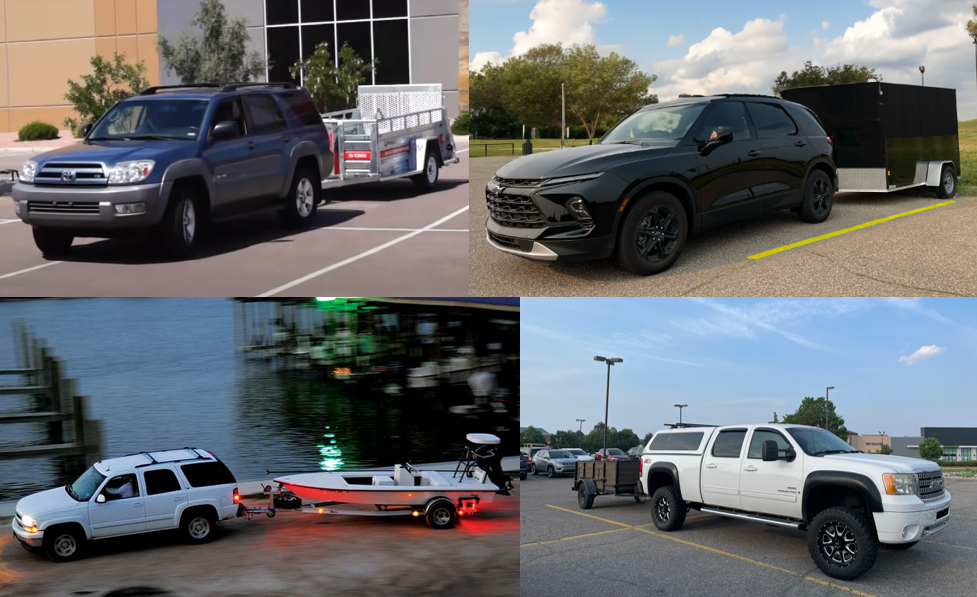
\includegraphics[scale=0.5]{fig/trailer_parking_real_world_all.png}
\caption{Truck trailer system in daily life}
\label{fig: real world trailer parking}
\end{figure}

Among the various features of ADAS, the control and auto-parking assist systems for tractor-trailer wheeled robots (TTWR) have gained significant attention in recent years, because of trailer vehicles' ability to significantly increase load capacity at a relatively low cost, resulting in more efficient use of resources and reduced transportation costs for achieving cooperative tasks\parencite{liu2022review}. However, the nonlinear, nonholonomic, unstable, and under-actuated system behaviors, along with the large blind zone behind the trailer make TTWR reverse parking a challenging and stressful experience. Another difficult part of the system is the phenomenon called jackknife, which occurs when the angle between the tractor and trailer is beyond a certain threshold, which prevents the driver from steering or aligning the trailer properly during driving backward. When the TTWR system is in the jackknife state, the steering maneuver has little effect on controlling the trailer's states.

Extensive research, for decades now, has been dedicated to addressing the challenges associated with TTWR systems, resulting in the development of various controlling methods that use controllers such as fuzzy logic, neural networks, and nonlinear controllers. For example, traditional control techniques, including Proportional-Integral-Derivative (PID) and model predictive controllers, have been widely utilized in Jackknife prevention, as well as other systems such as steer-by-knob. Jing et. al \parencite{jing2019control} solved the tractor-trailer reverse motion by designing three distinct controllers using a proportional integral controller, a sliding mode controller, and a neural network controller respectively. Moreover, a generic control safety governor was developed to supervises the tracking algorithms, overriding control to ensure jackknife-free operation. Xu et. al \parencite{xu2023improving} revisited Proximal Policy Optimization (PPO), enhancing it through two main innovations: firstly, they reformulate PPO into a linearly combined form to control the trade-off between accumulative discount return and divergence, addressing parameter tuning complexities, and secondly, they introduce a parametric alpha divergence in place of the traditional Kullback–Leibler (KL) divergence for more effective policy differentiation. The novel variant, alphaPPO, is validated across six benchmark environments, outperforming existing PPO forms. The work contributes a more effective balance in return and divergence, and a refined divergence measurement, broadening PPO's application in reinforcement learning. Zanchetta et. al \parencite{zanchetta2019trailer} propose a method to control the trailer's lateral position through vehicle yaw moment control, and by employing a control allocation algorithm and considering various constraints such as actuator limits and tire saturation, they present a robust solution for trailer control. This study extensively uses simulations, validated with real-world experimental data, to demonstrate the effectiveness of the method. This research contributes to the field of autonomous driving, specifically enhancing trailer control, and offers a novel approach that could be applicable to various vehicle configurations and driving conditions.

As technology evolves, especially in recent years, the application of machine learning algorithms for ADAS has emerged as a key element in the automotive industry for autonomous driving, as well as driver comfort and safety. Deep reinforcement learning has shown great potential for handling decision-making and controlling problems \parencite{ye2020automated}. It has become a popular research topic, in the field of continuous control development, for its flexibility and potential for improved control performance through trial and error. Unlike traditional supervised learning methods, deep reinforcement learning agents learn control policies through interactions within that environment, making them suitable for dynamic and unpredictable environments that are encountered in various applications such as autonomous driving and robotics \parencite{brunton2022data}. Several ADAS problems have been tackled using reinforcement learning algorithms \parencite{chen2019crowd}\parencite{du2020trajectory}\parencite{jaritz2018end}, but the development of end-to-end autonomous reverse parking systems for TTWR is still an ongoing area of investigation and growth. To overcome the limitations of rule-based models, which are prone to failures in unknown environments, Du et. al \parencite{du2020trajectory} present a novel trajectory planning method for automated parking systems using Deep Q-Network (DQN) learning, they apply the DQN algorithm to generate optimal paths in complex parking scenarios, considering the vehicle's nonholonomic constraints. Wang et. al \parencite{wang2021policy} propose a policy gradient reinforcement learning method specifically for reverse motion control of tractor-trailer mobile robots. Utilizing a continuous action space, the authors focus on the backtracking control problem and the challenge of jackknifing prevention, they employ a deep deterministic policy gradient (DDPG) algorithm to generate continuous control actions, thus providing an innovative approach to the problem. Through extensive simulations and comparison with other methods, the paper validates the effectiveness of the proposed approach in enhancing stability and safety during reverse driving of tractor-trailer systems. Bejar et.al \parencite{bejar2019preview} developed a preview neuro-fuzzy controller based on deep reinforcement learning for truck-trailer vehicle systems, and the research method includes utilizing a deep deterministic policy gradient algorithm integrated with a fuzzy logic rule-based system to train the controller. By combining deep reinforcement learning with neuro-fuzzy control, the safety performance and jackknifing avoidance are significantly improved. The paper demonstrates the application of modern machine learning techniques to a complex control problem, providing a new perspective on trailer vehicle control.

Model-based deep reinforcement learning (MBDRL) combines the benefits of deep learning with model-based control techniques, offering a novel approach for vehicle control. Unlike model-free methods that requires extensive interactions with the environment, MBDRL achieves proficient policies with fewer samples by utilizing a learned model of the environment. This model aids in simulating potential future outcomes, enabling the algorithm to anticipate and make informed decisions. While this "thinking ahead" capability enhances efficiency, it's essential to ensure the model's accuracy, as any discrepancies between the learned model and the real-world environment can lead to suboptimal or even erroneous control actions.

To conclude, the truck trailer wheeled robot systems present unique challenges compared to traditional cars and trucks. Their larger size and inherent instability during reverse movements make the task of crafting efficient motion planning and feedback control mechanisms especially complex, especially in the context of autonomous reversing. Modern solutions using deep reinforcement learning and neural networks offer innovative ways to enhance trailer movement performance. Leveraging AI-based techniques, these approaches can learn from complex driving scenarios and adapt to unforeseen conditions, thereby improving safety. Furthermore, the implementation of end-to-end parking solutions, driven by artificial intelligence, can significantly enhance user experience and efficiency by automating intricate parking maneuvers and allowing for a more seamless integration with existing transportation infrastructures. The combination of classical control algorithm and intelligent algorithms is opening new possibilities for handling these intricate control challenges, enabling more robust and responsive systems.

% Chapter 2
\chapter{\leavevmode\newline Motivation and Research Objective}
\label{chap:chapter_2}

The research objective of the truck trailer wheel robot (TTWR) system is to harness the potential of model-based deep reinforcement learning to achieve end-to-end control, with a focus on enhancing efficiency, stability, and real-world applicability. The main goals and key components of this research include:
\begin{enumerate}
   \item Building Trailer Movement State Equations: Developing precise mathematical models to represent the state dynamics of the TTWR system. This foundational work will create a framework for subsequent control and planning algorithms.
   \item Comparison of Classical Path Planning Methods: Investigating and comparing different classical path planning methods, including:
   \begin{itemize}
     \item Polynomial curve: One of the most simple and popular methods used in nowadays industrial and research field due to its computational efficiency and robust performance, it also provides a flexible framework that can be easily adapted to various requirements
     \item Clothoid curve: Providing smooth transitions between curves of different curvatures, which property makes it an ideal choice for applications such as road design, robotics, and autonomous vehicle navigation, where smooth and continuous paths are often desired.
     \item Dubins curve: Exploring its applicability for smooth path generation. The popularity of this algorithm is because of its simplicity and analytical tractability, and the algorithm also considers the physical constraints of the vehicle, such as its minimum turning radius.
     \item A* search: Analyzing its efficiency in finding optimal paths in complex environments. The A* search is an extension of Dijkstra's algorithm, with the added capability of using a heuristic to estimate the cost from the current node to the goal, allowing it to find optimal paths more efficiently.
   \end{itemize}
   \item Comparison of Different Control Algorithms: Conducting a comparative study of different control algorithms to identify the most effective approach for the TTWR system, including:
   \begin{itemize}
     \item PID: Evaluating its robustness and simplicity. Although PID controllers are simple, well-understood, and widely used in various industries,and hey are computationally efficient and work well for systems with known and stable dynamics, the tuning of PID parameters can be challenging, especially for complex or nonlinear systems. PID controllers may not handle disturbances or model uncertainties well, and they may require manual re-tuning if system dynamics change.
     \item LQR: Assessing its ability to handle nonlinear TTWR systems. Because LQR is mainly optimal for linear systems, providing robust performance by minimizing a quadratic cost function. It can handle multi-input and multi-output systems and can be designed to meet specific performance criteria. But when for nonlinear model, the lionization will cause inaccuracy because the LQR algorithm requires a precise mathematical model of the system and assumes linearity, moreover, designing and solving the underlying optimization problem can be computationally intensive.
     \item MPC: Analyzing its potential to handle constraints and model nonlinearities. The advantage of MPC is that the consideration of future states by solving an optimization problem at each step, allowing it to handle constraints and adapt to changes in system dynamics. But it requires a detailed mathematical model and can be computationally demanding, especially for high-frequency or real-time applications. The optimization problem must be solved at each time step, which may lead to challenges in implementation and tuning.
   \end{itemize}
   \item Implementation of Model-Free Reinforcement Learning: Implementing and evaluating different model-free reinforcement learning algorithms, such as:
   \begin{itemize}
     \item DQN: Investigating its effectiveness in discrete action spaces. DQN combines Q-learning with deep neural networks, enabling the handling of high-dimensional input spaces. It's robust and has been successfully applied to various tasks, especially in discrete action spaces. However, the continuous action spaces and instability during will be a problem in real world scenario training. The experience replay buffer required can be memory-intensive.
     \item DDPG: DDPG extends the ideas of DQN to continuous action spaces by combining Q-learning with policy gradients. It has shown success in various complex environments. But DDPG can be sensitive to hyperparameters and might suffer from training instability. It requires careful tuning and normalization techniques to achieve optimal performance.
     \item TD3: Assessing its ability to achieve stable learning in complex environments. TD3 improves upon DDPG by addressing overestimation bias and instability. It introduces a clipped double-Q learning and delayed policy updates, leading to more stable and efficient training. TD3, while more stable than DDPG, still requires careful hyperparameter tuning. The additional complexity in the algorithm might increase the implementation difficulty compared to simpler methods like DQN.
   \end{itemize}
   \item Implementation of Model-Based Reinforcement Learning: Implementing and evaluating different model-based reinforcement learning algorithms, such as:
   \begin{itemize}
     \item MBRL with known model \cite{sprayberry2023data}: where we plan over a known model, and only use learning for the global solution. The learnt model is based on classical trajectory planning including A*, RRT, or Dubins path, and after integrated with TTWR physical model, the model will generate TTWR trajectory states for the controller to take as input. The model-free RL algorithm will be used for the agent to interact with the environment, which is shown in figure \ref{fig: MBRL based on known model}
     \item Model-based RL with a learned model, where we both learn a model and learn a global solution.
   \end{itemize}
\end{enumerate}

\begin{figure}[h]
\centering
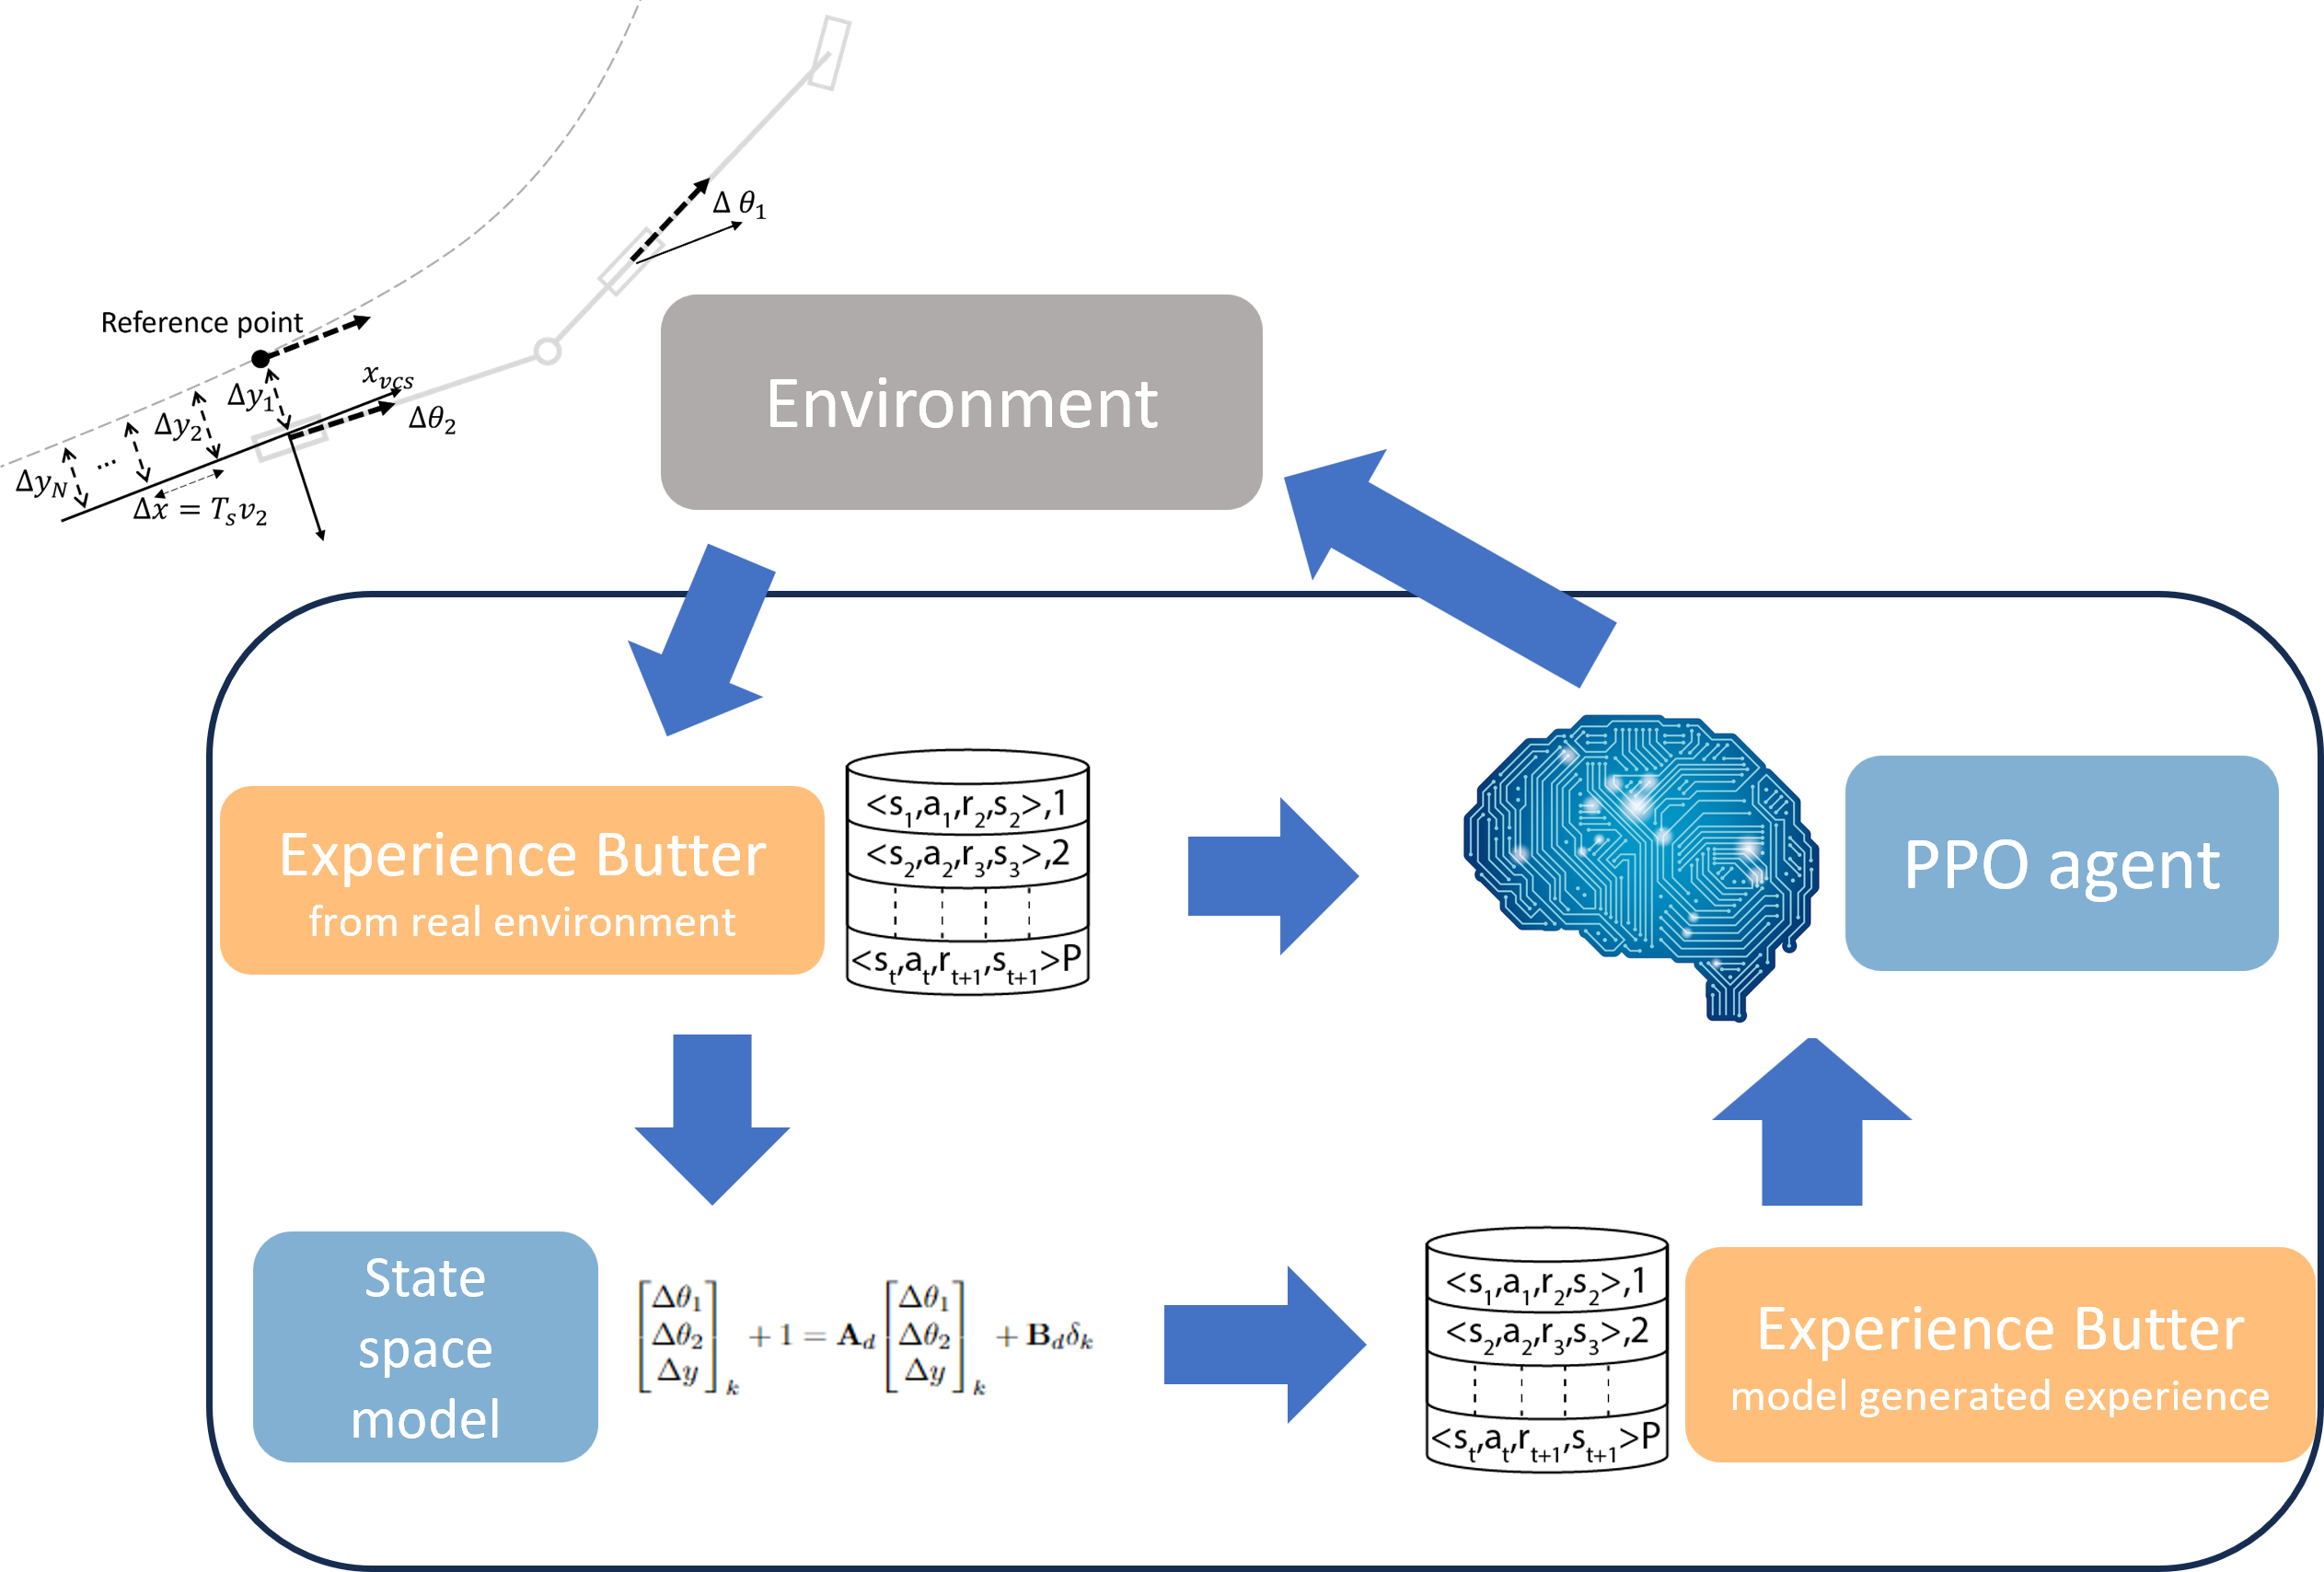
\includegraphics[width=0.8\linewidth]{fig/known mbrl schema.png}
\caption{MBRL based on known model}
\label{fig: MBRL based on known model}
\end{figure}

The proposed research aims to introduce a noval approach using model-based reinforcement learning for end-to-end control in truck-trailer wheel robot systems. While this is an exciting direction, it comes with its own challenges:

\begin{enumerate}
   \item World State Representation: Effectively representing the world states, including surrounding objects, system states, and movement cost, is a complex task that requires innovative methods to capture all relevant information without overwhelming the computational resources.
   \item Stability of Reinforcement Learning Algorithm: Ensuring the stability of the reinforcement learning algorithm, especially in the face of non-stationary and unpredictable real-world scenarios, is a critical challenge. Fine-tuning the balance between exploration and exploitation and devising robust training techniques will be essential.
   \item Computational Efficiency in Complex Environments: Designing computationally efficient methods that can be deployed in complex real-world environments without sacrificing performance or safety is a significant hurdle. Developing lightweight models and optimizing computation will be key to the successful implementation of the TTWR system.
\end{enumerate}

This research aims to make significant improvements in the control and automation of TTWR systems. By tackling the challenges and focusing on modern AI-based solutions, the goal is to enhance safety, efficiency, and adaptability in autonomous vehicles and complex robotic systems. The success of this work could lead to practical applications that are more responsive and reliable, improving efficiency of daily transportation and optimize energy usage.

% Chapter 3
\chapter{\leavevmode\newline Research background}
\chaptermark{Heading on Chapter Pages}
\label{chap:chapter3}

In the past decade, advancements in sensor and hardware capabilities have brought the concept of autonomous vehicles closer to realization. The popularity of events including the DARPA Grand Challenges \parencite{buehler20072005}\parencite{buehler2009darpa} has motivated major automotive companies and tech companies to further develop self-driving technology and deploy such technologies in daily life scenario. The potential benefits of eliminating human intervention in driving are manifold, which aims to enhance road safety, reduce traffic congestion, decrease carbon emissions, and offer mobility to those unable to drive. It represents a shift towards sustainable and efficient transportation, potentially transforming urban planning, energy consumption, and societal accessibility. Such technological strides not only offer car companies an opportunity to differentiate themselves in a competitive market but also align with the increasing demands of the transportation sector. With transportation being a significant contributor to global carbon emissions, regulatory bodies such as the European Road Transport Research Advisory Council and the European Commission have delineated ambitious targets. Their vision is to achieve a $50 \%$ enhancement in transport efficiency by 2030, relative to 2010, and simultaneously curtail emissions by $60 \%$. 

Nowadays, Advanced Driver Assistance System (ADAS) has been developed to enhance road safety by aiding drivers in maintaining vehicle stability, and has emerged as a bridge between today's vehicles and the future of full autonomy. While classical perception, path planning, and motion control methods can handle the majority of driving scenarios, there remain certain corner cases where these traditional techniques fails. These complex and often unpredictable scenarios present unique challenges that cannot be easily resolved using conventional approaches. As a result, the modern ADAS algorithm integrates various sensors and algorithms to assist drivers, making driving safer and more efficient. From simple parking assistance to complex adaptive cruise control, these systems represent the intersection of robotics, artificial intelligence, and vehicular engineering and try to create more sustainable, efficient, and safer transportation solutions.

Compared with vehicles which does not have additonal trailer connected to the ego vehicle body, the truck-trailer wheeled robot, have always brought challenges to the classical state estimation and control methods. While there has been significant progress in developing state and parameter estimation techniques for single-unit vehicles, the area of vehicle-trailer system state and parameter estimation still can be explored, and especially when considering the task of reverse driving. The dynamics involved in reversing a truck-trailer system differ significantly from those of forward driving, primarily due to the inherent instability and non-holonomic constraints (constraints that are non-integrable into positional constraints) of the system. When a truck attempts to reverse with a trailer, the angle between the truck and trailer can quickly grow uncontrollable, leading to a phenomenon known as jack-knifing.

In the previous research, control of such systems was the domain of skilled human operators; however, with the advent of automation and the push towards autonomous vehicles to wider user scenario, there has been a growing interest in developing algorithms that can reliably and safely control truck-trailer systems during reverse driving. Traditional control methods, such as Proportional-Integral-Derivative (PID) controllers, Linear Quadratic Regulators (LQR), and Model Predictive Control (MPC), have been explored for this purpose. While these methods have seen success, they often rely on accurate models of the system dynamics and can struggle with the nonlinearities and uncertainties from the real-world driving scenarios. In recent times, methods that take advantage of modern machine learning techniques, such as deep reinforcement learning , have been introduced, which combines the capabilities of deep learning for recognizing complex patterns with reinforcement learning for decision-making. This fusion enables systems to learn and adapt through continuous interaction with complex environment and adjust its strategy to achieve optimal control.

\section{Overview of path planning}

Historically, path planning was primarily based on geometric and grid-based methods. Geometric methods, such as the Voronoi diagram, partitioned the workspace into regions to find the safest path. Grid-based methods, on the other hand, divided the environment into a grid and used search algorithms to find the path. However, these methods often faced challenges in complex environments or when high precision was required. One of the most popular methods used in autonomous parking is Dubins curve, which is named after Lester Eli Dubins, is a mathematical solution that provides the shortest curve between two points in the plane with a constraint on the curvature. While the Dubins Curve itself was introduced in the 1950s, and with an assumption that the vehicle traveling the path can only travel forward. If the vehicle can also travel in reverse, then the path follows the Reeds–Shepp curve \parencite{reeds1990optimal}, its application to automated parking has been a more recent development, and its integration into parking algorithms allowed for smooth and efficient paths that adhered to the nonholonomic constraints of vehicles, such as a fixed minimum turning radius.

\begin{figure}[h]
\centering
\resizebox{\textwidth}{!}{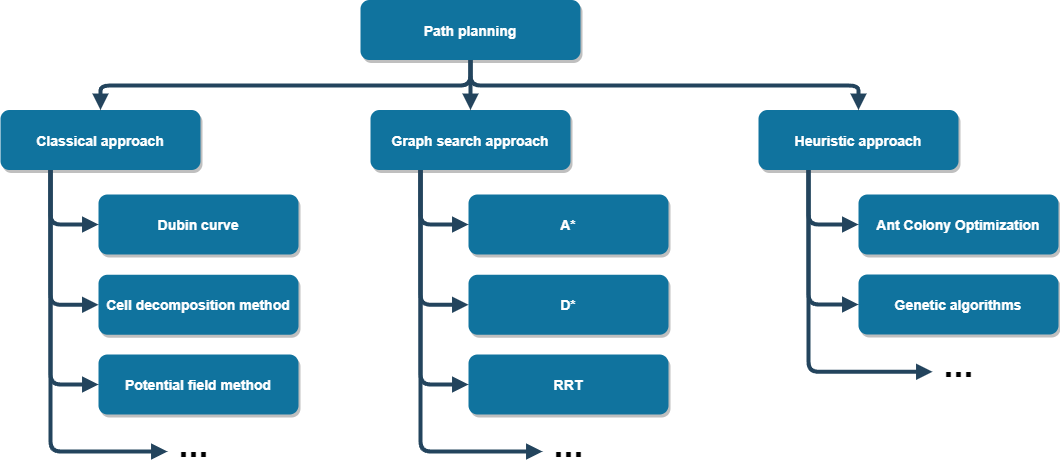
\includegraphics{fig/path_planning_map.png}}
\caption{Map of path planning methods}
\label{fig: path planning map}
\end{figure}

Nowadays, graph search algorithms are becoming dominantly popular and are fundamental to path planning, as they provide systematic ways to explore and navigate through a network of nodes and edges representing the environment. The most basic graph search algorith is Dijkstra algorithm \parencite{dijkstra2022note}, and it has been a foundational method commonly used in applications like Google Maps, known for its guaranteed optimal solutions but criticized for its computational intensity in blind searches. However, the computational-intensity limits the Dijkstra’s blind searches capability, and as a result A* \parencite{hart1968formal} and its variants are becoming the state of the art algorithms for use within static environments, they combined the benefits of both, using a heuristic to guide the search towards the goal while also considering the actual cost from the start. A* guarantees to find the shortest path if an admissible and consistent heuristic is used, and by using a heuristic that estimates the cost to the goal, A* often explores fewer nodes than algorithms like Dijkstra's, making it more efficient in many cases. The A* algorithm and its variants are a significant milestone in the field of path planning, because the balance between efficiency and optimal helped the industry to reduce cost and improve stability.

However, A* and A* re-planner are used for shortest path evaluation based on the information regarding the obstacles present in the environment, and the shortest path evaluation for the known static environment is a two-level problem, which comprises a selection of feasible node pairs and shortest path evaluation based on the obtained feasible node pairs \parencite{dudi2020shortest}. Both of the above mentioned criteria are not available in a dynamic environment, which makes the algorithm inefficient and impractical in dynamic environments. To support path planning in dynamic environments, D* \parencite{stentz1994optimal} and its variants are discussed as efficient tools for quick re-planning in cluttered environments. As D* and its variants do not guarantee solution quality in large dynamic environments, we also explore Rapidly-exploring Random Trees (RRTs) \parencite{lavalle1998rapidly} and a hybrid approach combining Relaxed A* ( RA*) \parencite{ammar2016relaxed} and one meta-heuristic algorithm. The hybrid approach comprises two phases: the initialization of the algorithm using RA* and a post-optimization phase using one heuristic method that improves the quality of solution found in the previous phase. Three meta-heuristic algorithms are also discussed: namely, the Genetic, Ant colony, and Firefly algorithms. These are aimed at providing effective features in pursuit of a hybrid approach to path planning.

The A* algorithm, although effective in static environments, its application in dynamic settings is hindered by its two-level problem structure, involving the selection of feasible node pairs and path evaluation based on these pairs. This makes A* less practical in ever-changing environments. To address the challenges in dynamic environments, incremental versions of A* such as the D* algorithm have been developed, allowing for path updates as new information becomes available1. However, D* and its derivatives may not always ensure solution quality in extensive dynamic landscapes \parencite{stentz1994optimal}. D* is designed to handle changes in the environment, allowing for efficient replanning without having to restart the search from scratch, and it is able to reuse the previous computations, and efficiently update the solution when changes occur, making it suitable for real-time applications. However, D* and its derivatives may not always ensure solution quality in extensive dynamic landscapes, and as result, A rapidly exploring random tree (RRT) is designed to efficiently search nonconvex, high-dimensional spaces by randomly building a space-filling tree. 

Path planning is a critical aspect of autonomous driving and ADAS, guiding the ego vehicle go through complex environments. Algorithms like Dubins curve, Dijkstra's, A*, RRT, and D* are chosen as they represent different facets of path planning, serving as various scenarios from static to dynamic environments, and from deterministic to probabilistic approaches. The trend of integrating AI, particularly machine learning, into path planning is reshaping the field. By leveraging data-driven insights and adaptive algorithms, AI-enhanced path planning offers the potential for more robust, efficient, and intelligent navigation. This fusion of traditional algorithms with AI techniques signifies a promising direction for future innovation and optimization in path planning \parencite{mcmahon2022survey}.

\section{Overview of vehicle control}

The evolution of control theory in autonomous driving and Advanced Driver Assistance Systems (ADAS) has been marked by the development and application of various control strategies, reflecting the complexity and diversity of the challenges in this field. 

\begin{figure}[h]
\centering
\resizebox{\textwidth}{!}{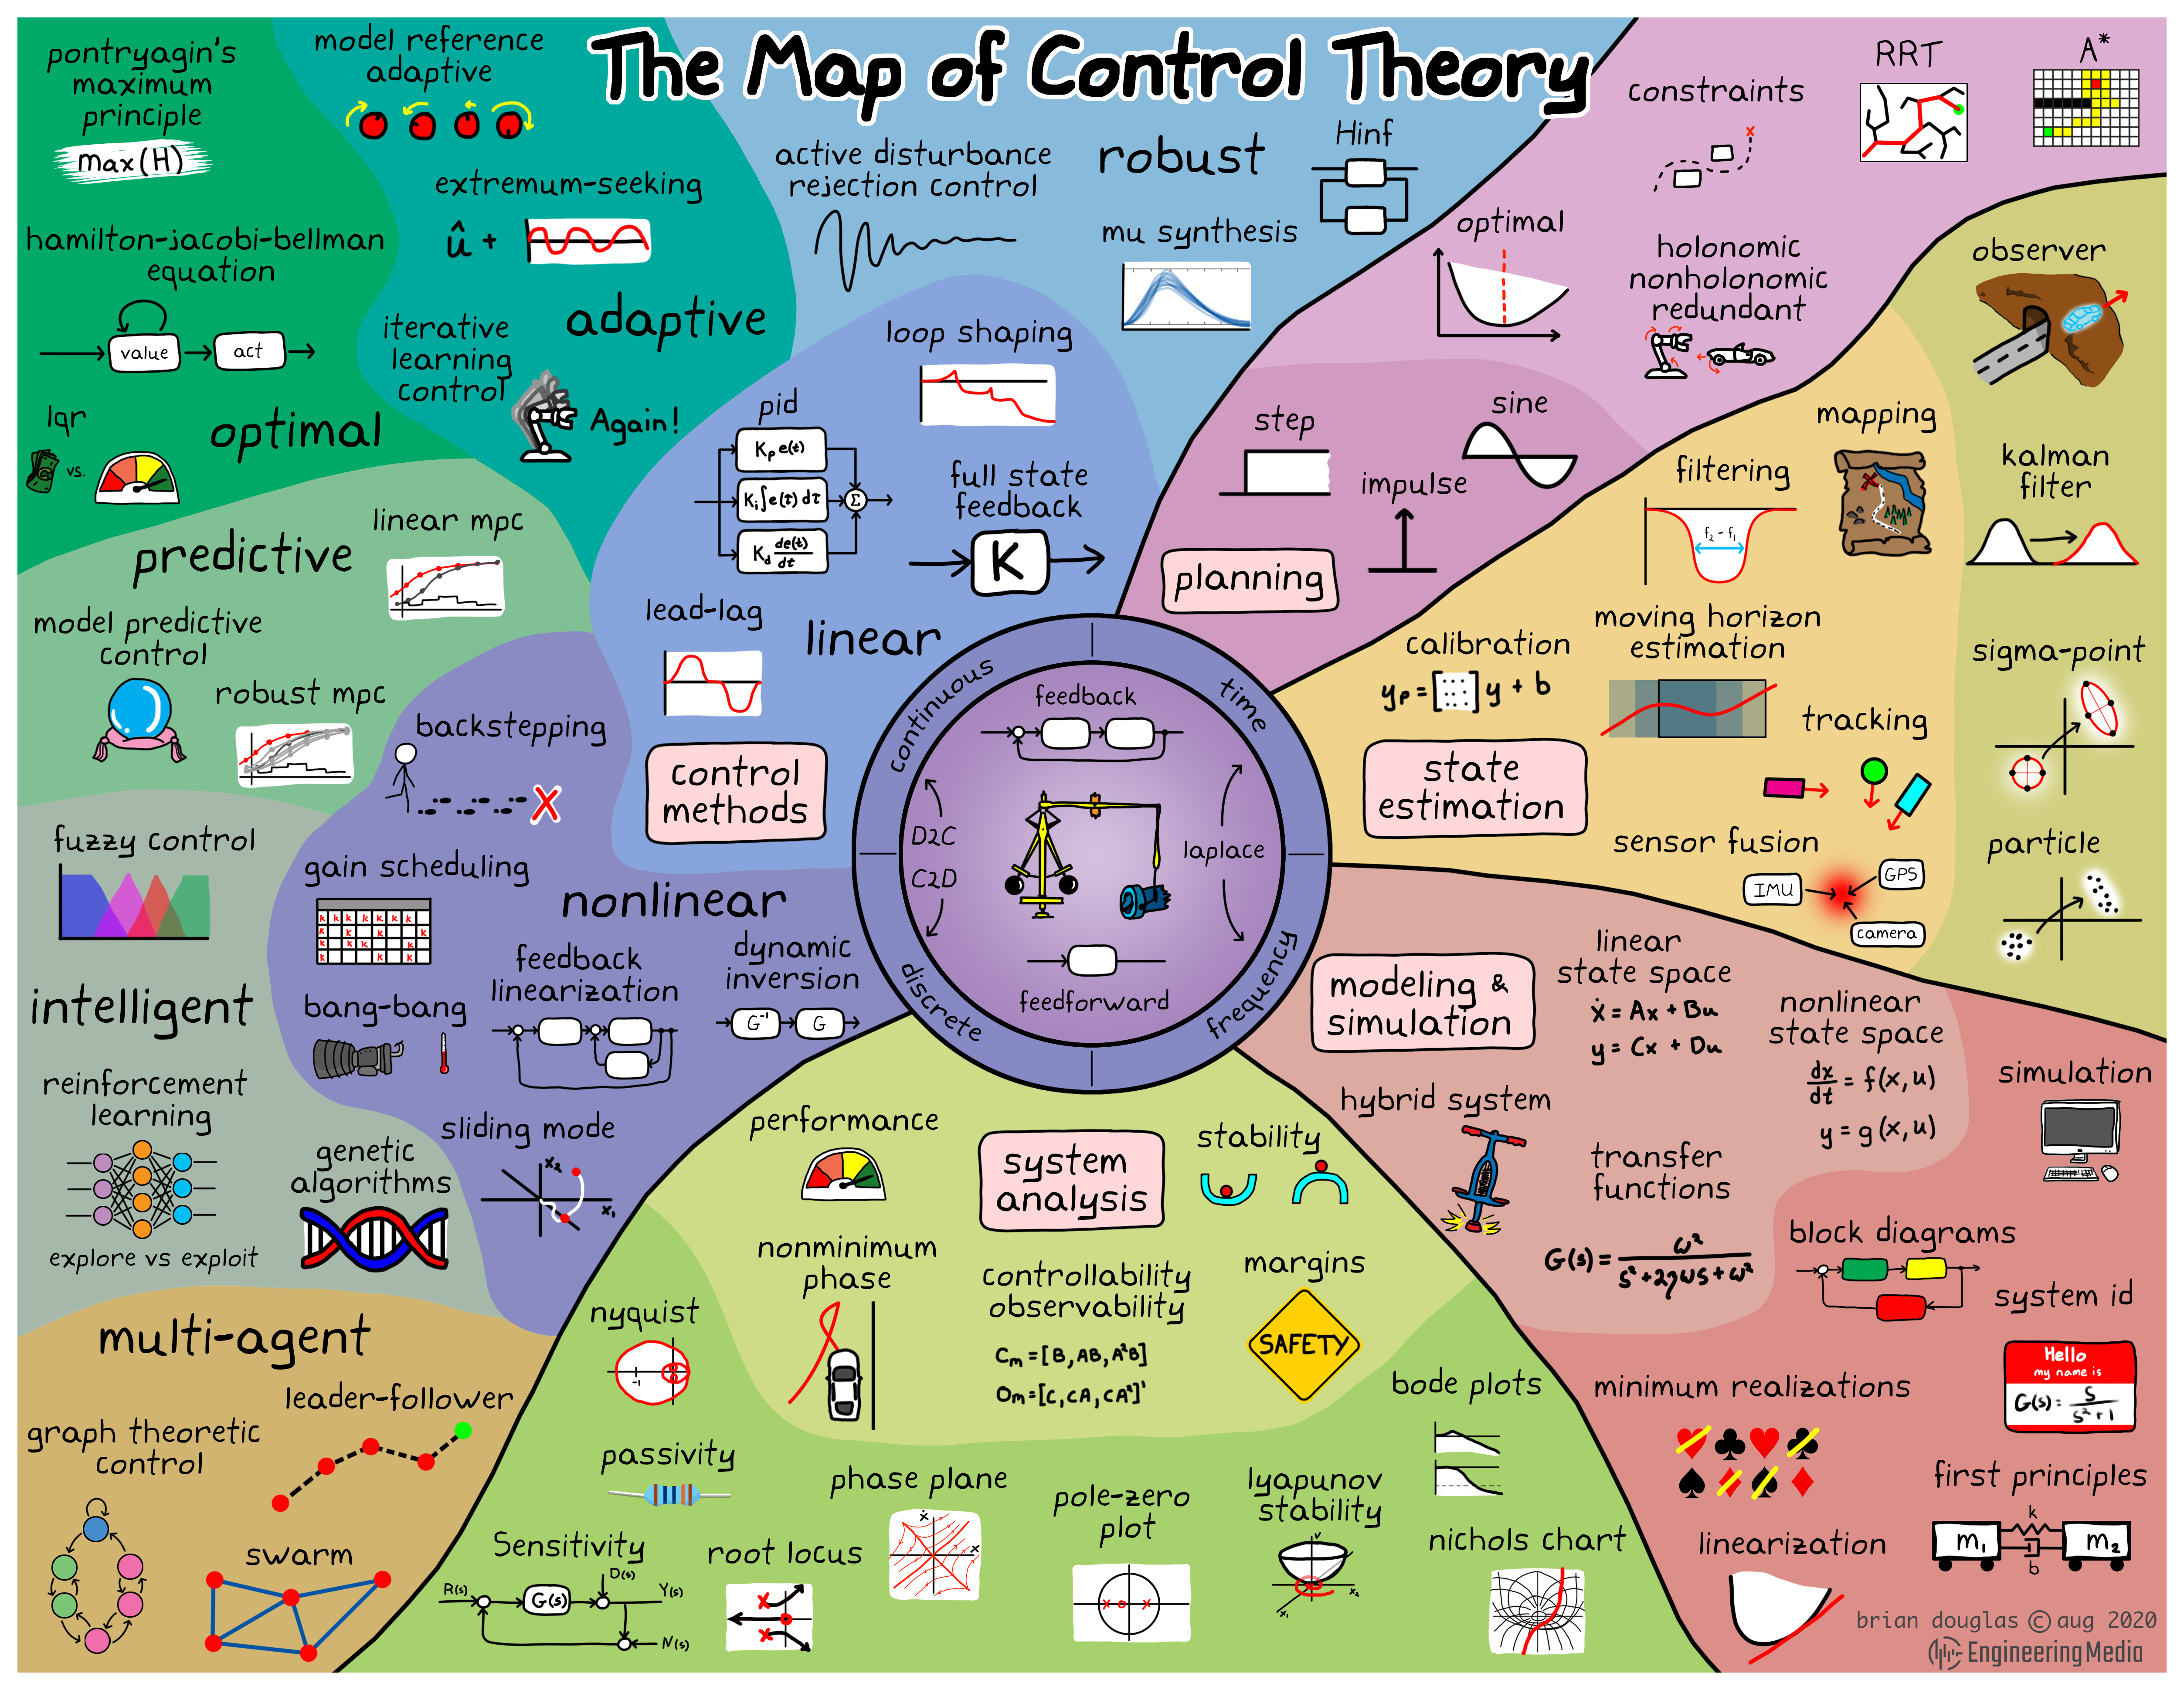
\includegraphics{fig/Control_Map_ver5.png}}
\caption{Map of control theory\parencite{EngineeringMedia}}
\label{fig: control map}
\end{figure}

Starting with PID control, which originated in the early 1920s, initially applied to automatic steering systems for ships. This marked the first theoretical analysis and practical utilization of PID in a real-world context. As the technology matured, it found its way into the manufacturing industry, where it played a vital role in automatic process control. Initially implemented in pneumatic controllers, it later transitioned to electronic formats. In the modern era, the PID concept has become a universal standard, employed across various fields and applications where precise and optimized automatic control is essential. Utilizing feedback control, PID controllers adjust actions based on the error between desired and actual states, making them suitable for tracking target velocity and lateral positioning in autonomous driving \parencite{bennett1996brief}. 

The main drawback of PID controllers is that every test on the actual system requires its linearization. For LQR control, this step is not needed, and one can directly feed in the system equations to the controller and get the desired response \parencite{saraf2020comparative}. As one of the optimal control theory which aims to operate a dynamic system at the lowest cost, the LQR controll can be appplied in the Linear Quadratic (LQ) problem, where system dynamics are defined by linear equations, and the cost is a quadratic function. By minimizing a cost function defined by deviations from desired values, like lateral distance or longitudinal velocity, the controller finds the optimal settings that reduce undesired deviations, and the control action's magnitude may also be part of the cost function.

LQR (Linear Quadratic Regulator) is limited by its assumption of a linear system, caused inconvenience for its application in real-world scenarios which are often highly nonlinear. In contrast, MPC (Model Predictive Control) is designed to handle nonlinear systems without the constraints of linearity. It can manage hard constraints and deviations from a linearized operating point, major drawbacks to LQR. Unlike LQR, which optimizes across the entire time horizon, MPC optimizes within a receding time window, frequently computing new solutions. This flexibility allows MPC to adapt to complex, nonlinear environments, making it more suitable for many real-world applications.

Another control method used widely is called fuzzy control, compared with PID control which requries techniques and algorithms to tune the PID gains by a skilled human operator during the application of the controller to a process, fuzzy control uses fuzzy sets and fuzzy rules to model complex systems. Unlike traditional binary logic, fuzzy logic allows for degrees of truth, representing values on a continuum rather than as absolute true or false. Fuzzy controllers translate these fuzzy sets into control actions, making them suitable for handling uncertainty and ambiguity. Because of its ability to handle imprecise information makes it flexible and applicable to various complex systems, it is becoming a popular choice, especially in applications where traditional PID control might struggle. It represents a more intuitive and adaptable control methodology, suitable for a wide range of real-world scenarios.

\section{Overview of end to end driving}

The concept of end-to-end autonomous driving has evolved from traditional hierarchical architectures to more streamlined and integrated approaches. Historically, autonomous driving systems were designed with complex, layered structures, including separate modules for environment perception, path planning, and motion control. The hierarchical scheme, as seen in Carnegie Mellon's BOSS car \parencite{urmson2008autonomous} and Stanford's Junior \parencite{buehler2009junior}, was prevalent in the early stages of autonomous driving development.

However, the rise of deep learning and reinforcement learning has paved the way for end-to-end methods. These approaches directly map raw sensor data to low-level control commands, bypassing the need for modularized design. NVIDIA's work in 2016 marked a turning point, realizing end-to-end autonomous driving on real-world freeways \parencite{bojarski2016end}, where an end-to-end deep learning approach to control an autonomous vehicle were demonstrated. Unlike traditional methods that relied on hand-crafted features and complex pipelines, NVIDIA's approach used a Convolutional Neural Network (CNN) to map raw pixels from a single front-facing camera directly to steering commands.

Comapred with traditional hierarchical architectures, which is complicated and hard to design, end-to-end methods offer a more straightforward structure, reducing the burden of designing complex modules. And the Adaptability of end-to-end approaches allows new scenarios to be learned by interaction and previous experienced to eb generalized at scale, unlike traditional methods prone to error propagation. Also, because all sensor data is directly used and mapped for driving, there's less perception information loss or error propagation, and the algorithm has the ability to find the correlations between different sensors. Nowadays, the imitation learning or reinforcement learning has been introduced and employed in end-to-end driving research, making it possible for vehicles to learn and improve end-to-end driving by themselves.

\begin{figure}[h]
\centering
\resizebox{\textwidth}{!}{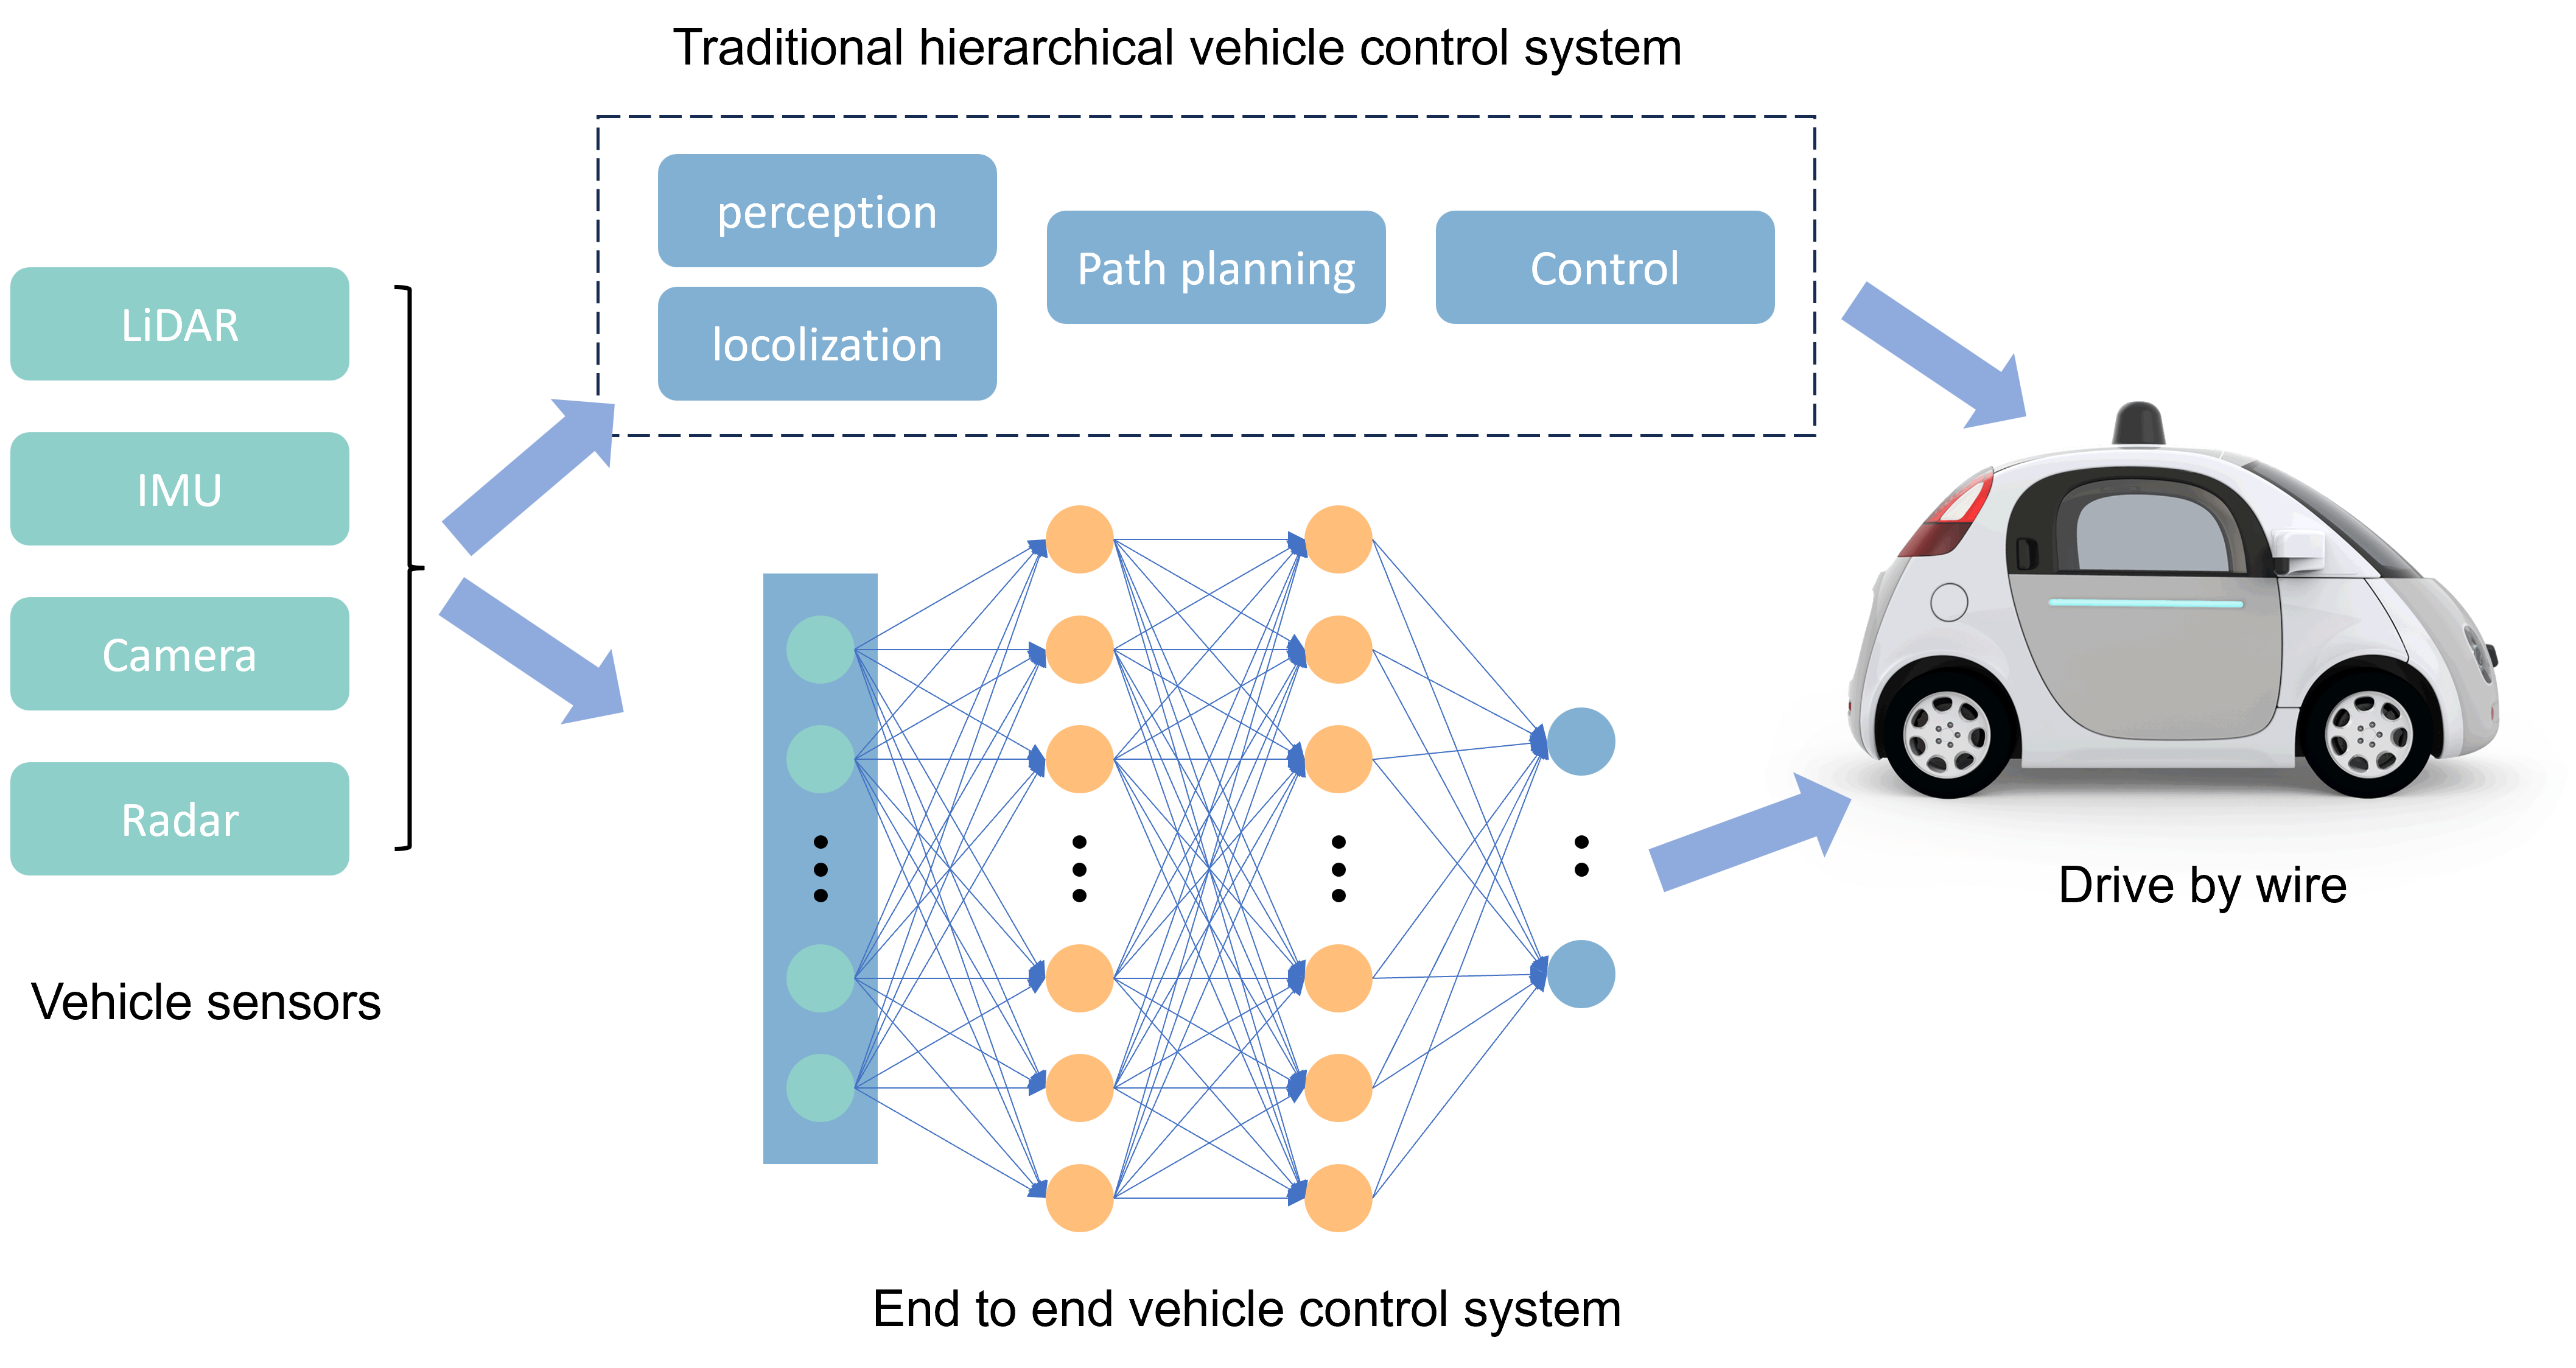
\includegraphics{fig/traditional_endToEnd.png}}
\caption{Comparison between traditional hierarchical vehicle control system and end to end vehicle control system}
\label{fig: traditional endToEnd}
\end{figure}

In the realm of end-to-end autonomous driving, various research methods have been employed to achieve seamless control and navigation. The work from Nvidia by using a Convolutional Neural Network to directly map raw pixels from cameras to steering commands has been a foundational approach, simplifying the control process by directly linking visual input to driving actions. Building on this, Imitation Learning (IL), or learning from demonstrations, has emerged as a technique where an agent learns the optimal policy by imitating expert human behavior, providing a data-driven way to capture complex driving strategies. Reinforcement learning has extend this idea further by mapping raw pixels to discretized actions, offering a more interactive and self improving control mechanism, which demonstrated successful results on real world driving recently, including lane following \parencite{kendall2019learning} and urban driving \parencite{jaritz2018end}. Peng et al \parencite{peng2021end} introduces an end-to-end autonomous driving approach utilizing the Dueling Double Deep Q-Network, a deep reinforcement learning algorithm. This method enables the vehicle to independently learn end-to-end driving, fostering self-reliance in navigation and control. Actor-Critic Methods, such as A3C, DDPG, and TD3, have been applied to handle complex decision-making and planning problems, integrating both value and policy-based learning for more robust control. Reinforcement learning has been successfully applied in autonomous driving when combined with supervised learning in recent years. The future of RL in autonomous driving faces challenges in transferring findings from simulation to the real world. Simplistic reward functions may encourage risky behavior \parencite{knox2023reward}, and designing or learning better functions remains an open problem. Combining RL with world models and enhancing representation learning are key areas for ongoing exploration and development. Also, current RL solutions for autonomous driving will be hindered by high dimensional representation due to computational cost, and research is still on going for the model to learn from and interact with the world in a more data efficient way \parencite{chen2023end}.

In conclusion, the end-to-end autonomous driving using Deep Reinforcement Learning has emerged as a promising direction, offering simplicity, adaptability, and the potential for superior performance. It stands in contrast to traditional hierarchical methods, providing a more integrated and flexible approach. However, challenges related to data dependency, interpretability, sensor integration, and robustness continue to be areas of active research and development. The ongoing exploration of various DRL algorithms, combined with real-world training and attention to interpretability, is shaping the future of autonomous driving, making it an exciting and dynamic field of study.

\section{Model based reinforcement learning in autonomous driving}

In reinforcement learning context, unlike other machine learning methods, the learning process is pushed forward using the interactions between the agent and the environment, which means the agent learns control mapping function directly from its surroundings without requiring supervision. However, discrimination between the agent and the environment is not always clear, which varies in different application. For instance, in autonomous driving problems, the vehicle's actuator response are often considered part of the environment.

The main difference between model-based and model free reinforcement learning is whether a model of the interactions between the robot and the environment is employed. MFRL algorithm learns the control policy without such model, and instead, it relies on the method called trial-and-error, which directly with the physical system to discern rewards and determine optimal actions. On the other hand, MBRL incorporates a model which captures the environment transition dynamics, and use this model as the foundation for reward determination and action optimization. Consequently, in model-based approaches, policies are fine-tuned using the model, and once optimized, they are then deployed on the actual system. This process is depicted in Figure \ref{fig: mbrl schema.png}, and shows the typical data flow of a model-based reinforcement learning approach.

\begin{figure}[h]
    \centering
    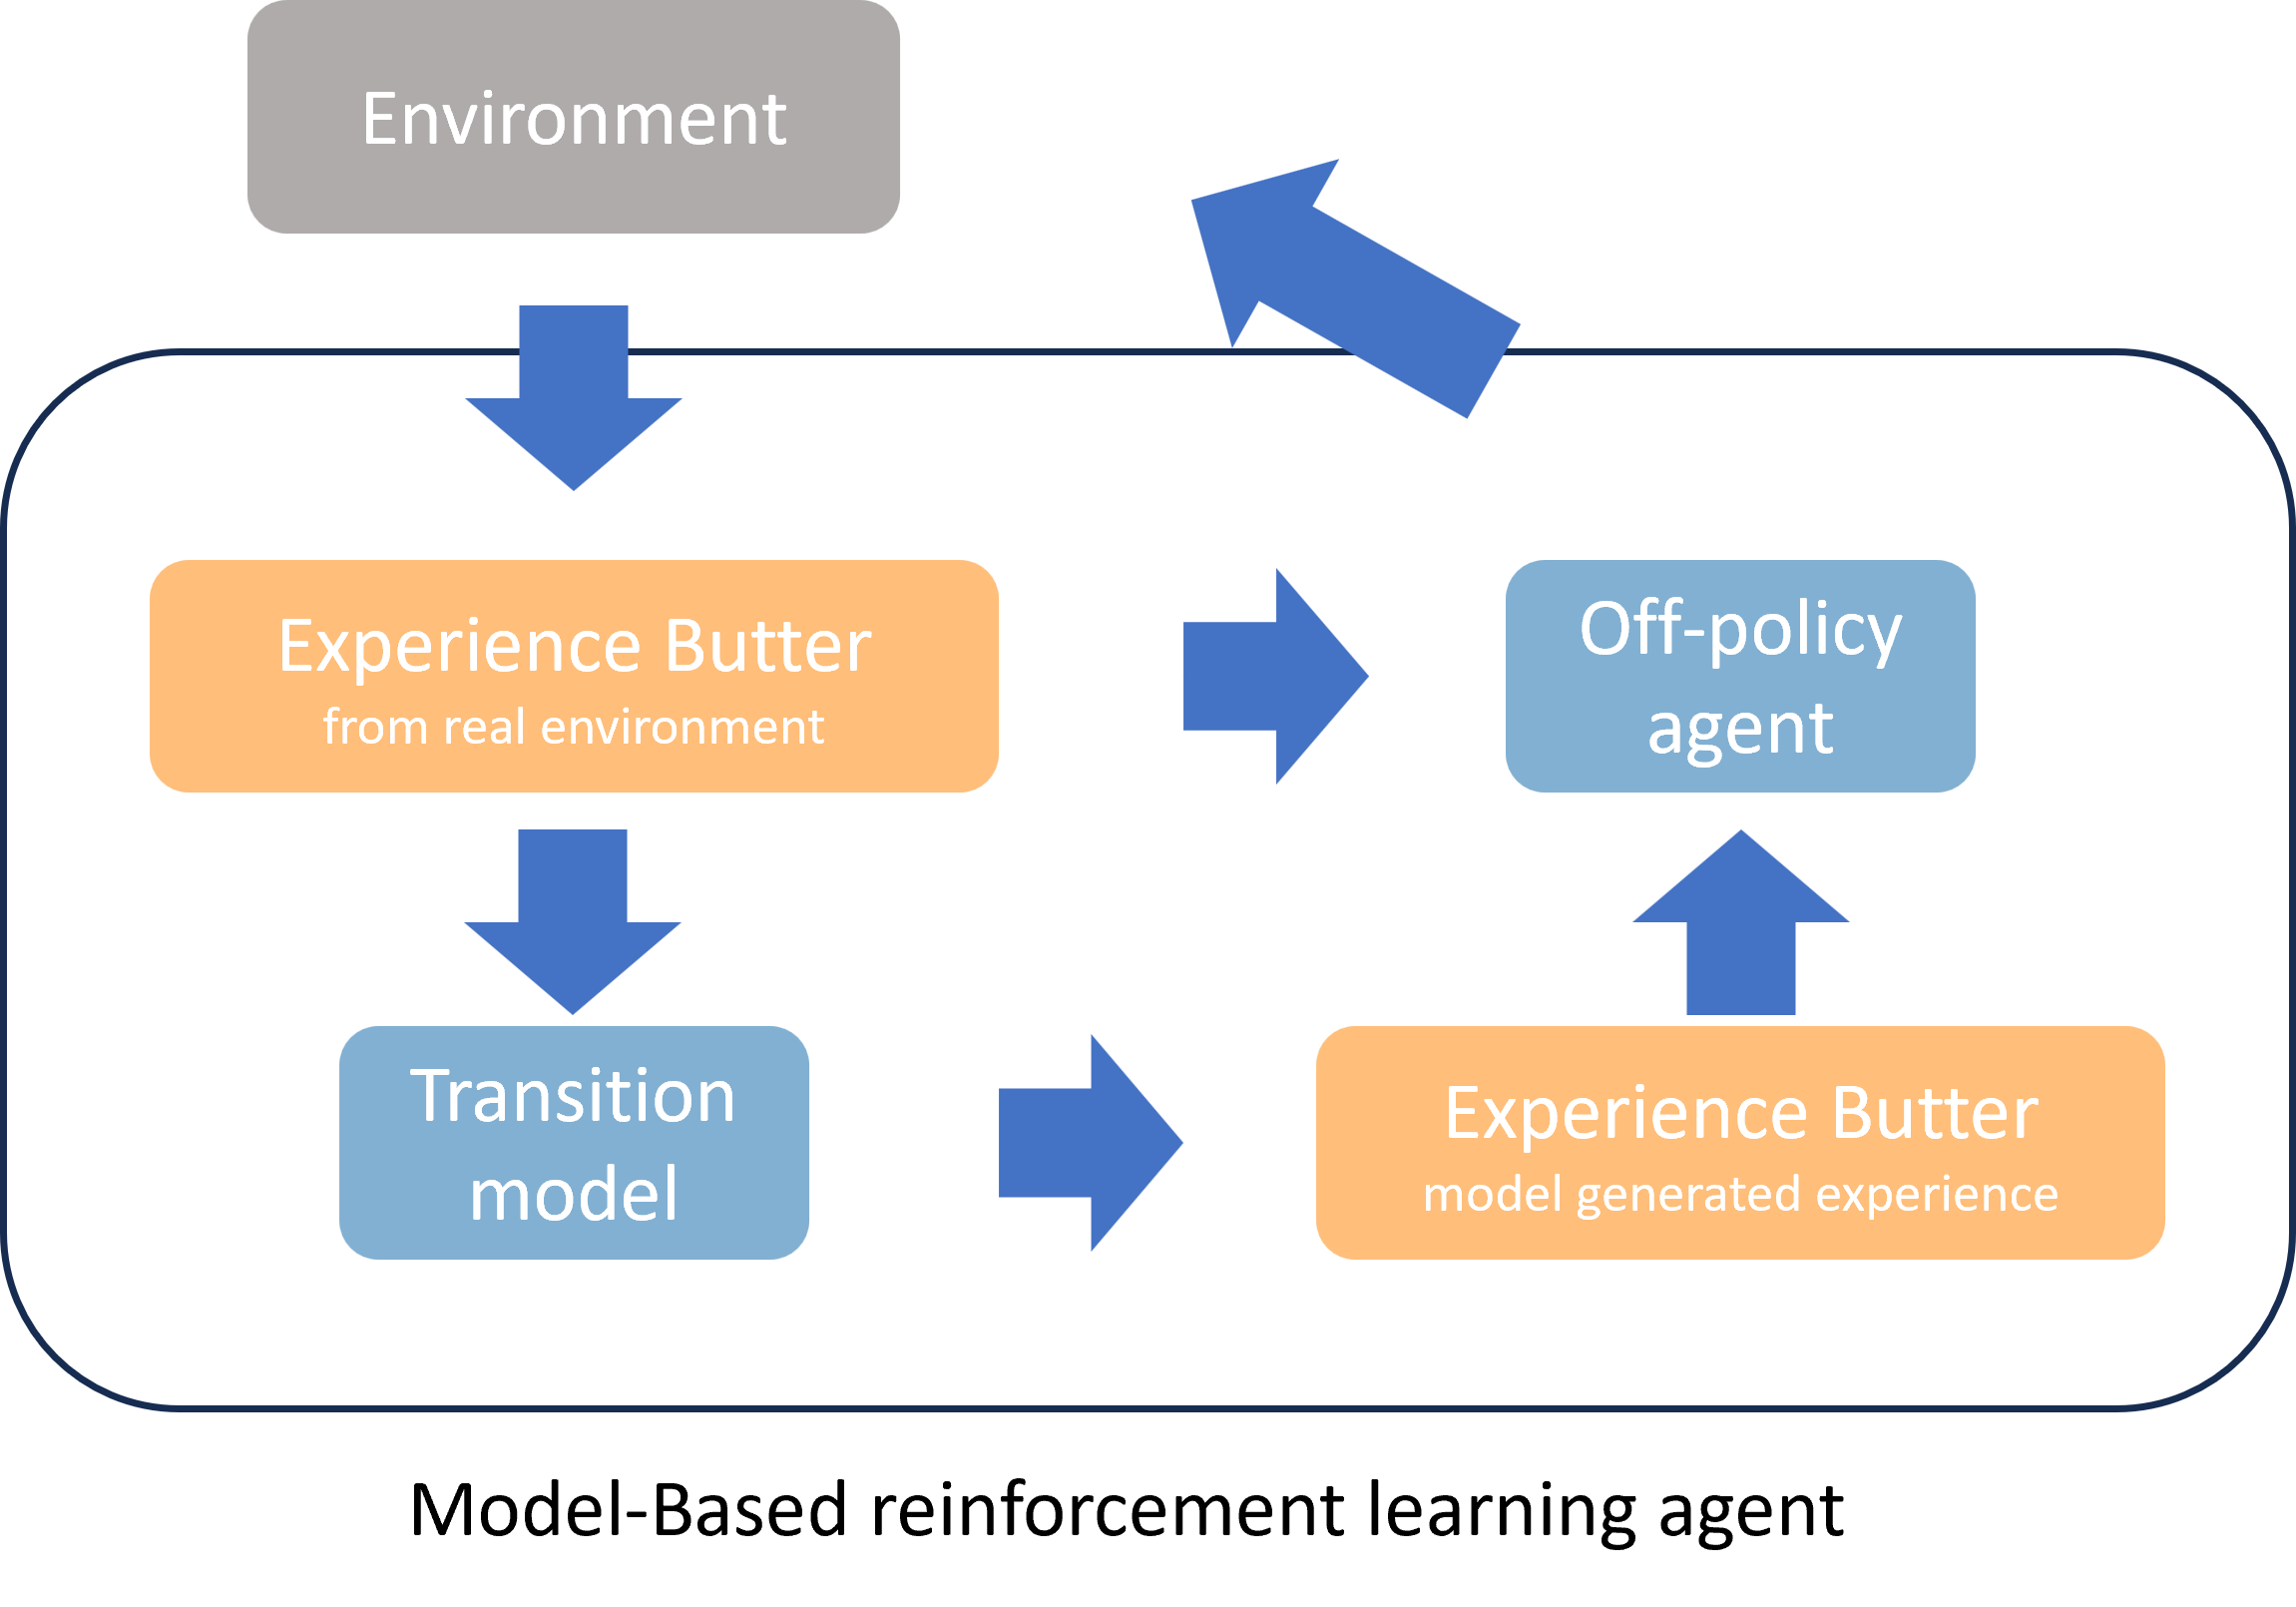
\includegraphics[width=0.7\textwidth]{fig/mbrl schema.png}
    \caption{Model-based reinforcement learning schema}
    \label{fig: mbrl schema.png}
\end{figure}

Nowadays, the model-based reinforcement learning has been proven to be sampling efficiency and wide adaptable in the field of robotics. Huang et. al. investigated the challenge of parametrizing
policies for reinforcement learning in highdimensional continuous action spaces, and present a practical model-based RL method leverages the multimodal policy parameterization and learned world model to achieve strong exploration capabilities and high data efficiency \parencite{huang2023reparameterized}. Hu et. al. introduces a model-based reinforcement learning technique for autonomous driving, which learns the world model and driving policy using 3D geometry from high-resolution expert videos. Trained offline on urban driving data, MILE outperforms previous methods by $31\%$ in the CARLA simulator under new conditions. It uniquely integrates static and dynamic scene modeling with ego-behavior using only cameras\parencite{hu2022model}. Heess et. al. introduced a unified framework for learning continuous control policies via backpropagation, developed multiple RL algorithms based on teh framework, and then compared the general policy gradient algorithms that range from model-free methods with value functions to model-based methods without value functions. The results showed that the model-based algorithm SVG(1) shows the effectiveness of learning models, value functions, and policies simultaneously in continuous domains comapred with other competators. 

To conclude, model-based reinforcement learning is becoming a popular research area as it requires fewer interactions with the environment compared to model-free RL, which reduced interaction not only minimizes the risk of accidents but also reduces wear and tear on the robot. To successfully implement MBRL, the transition models should be designed carefully, which will affect the performance of the learning algorithm in terms of accuracy and convergence. Furthermore, imitation learning combined with RL, by guided by human demonstrations, making RL a promising approach for tasks like autonomous driving where human-like decision-making is preferred.

% Chapter 4
\chapter{\leavevmode\newline TTWR state space analysis}
\chaptermark{TTWR state space analysis}
\label{chap:TTWR state space analysis}

This chapter outlines the main focus of the research, detailing the definition of the TTWR state space and its controllability analysis. The study employs a kinematic truck-trailer vehicle model to represent a simulation vehicle operating at low speeds without tire slip. While a comprehensive model might encompass vehicle dynamics, such as load transfer and tire slip, this research primarily centers on the kinematic aspects for low speed parking scenarios. The chapter concludes by addressing the limitations of the TTWR model and the common methods to avoid such issue.

\section{TTWR kinematics state space}

Previous research \parencite{sorge2019motion}\parencite{liu2019minimum} has provided various physical models for vehicle state analysis, including both kinematic and dynamic state models. The choice of model depends on the desired level of accuracy and the specific operating conditions. For high-speed driving tasks, the dynamic factors play a significant role in motion planning and vehicle control; however, in low-speed driving scenarios, the kinematic constraints have a greater influence on the motion behavior of the TTWR system. Since the TTWR reverse parking task is operated in low-speed driving conditions, the system model is established based on the kinematic relations. In this paper, we utilized the Ackermann chassis vehicle as the host vehicle, and the trailer employed a single-axle chassis for the TTWR system. The two vehicles in the system are linked by the hitch ball, which is a unique pivoting point. The pivot point enables the interconnected vehicles to execute relative rotational motion between each other. From a mechanical structure perspective, the tractor and the trailer can be regarded as two separate rigid bodies. The vehicle body structure exhibits symmetry with respect to the axis, with the left and right sides being symmetrical. On flat non-slippery ground and under low-speed driving, the side-slip caused by tires and control effect delay caused by mechanical or electrical units can be neglected\parencite{lei2021research}. In Table \ref{table: ttwr system states}, the major parameters of the TTWR system are listed.

\begin{table}
\centering
\caption{The TTWR system states}
\setlength{\tabcolsep}{12pt}
\begin{tabular}{|p{3cm}|p{9cm}|}
\hline
Parameters& 
Descriptions  \\
\hline
$x_1 $& 
The lateral position of the host vehicle \\
$y_1$& 
The longitudinal position of the host vehicle \\
$\theta_1$& 
The yaw angle of the trailer \\
$x_2 $& 
The lateral position of the trailer \\
$y_2$& 
The longitudinal position of the trailer \\
$\theta_2$& 
The yaw angle of the host vehicle \\
$\phi $& 
The host-trailer angle \\
$v$& 
The longitudinal velocity of host vehicle \\
$\delta $& 
The steering angle of host vehicle \\
$L_1$& 
The host vehicle wheelbase length \\
$L_2$& 
The rear overhang of the host vehicle from the rear axle to the hitch point \\
$L_3$& 
The overhang of the trailer from the the hitch to trailer axle \\
\hline
\end{tabular}
\label{table: ttwr system states}
\end{table}

\begin{figure}[h]
\centering
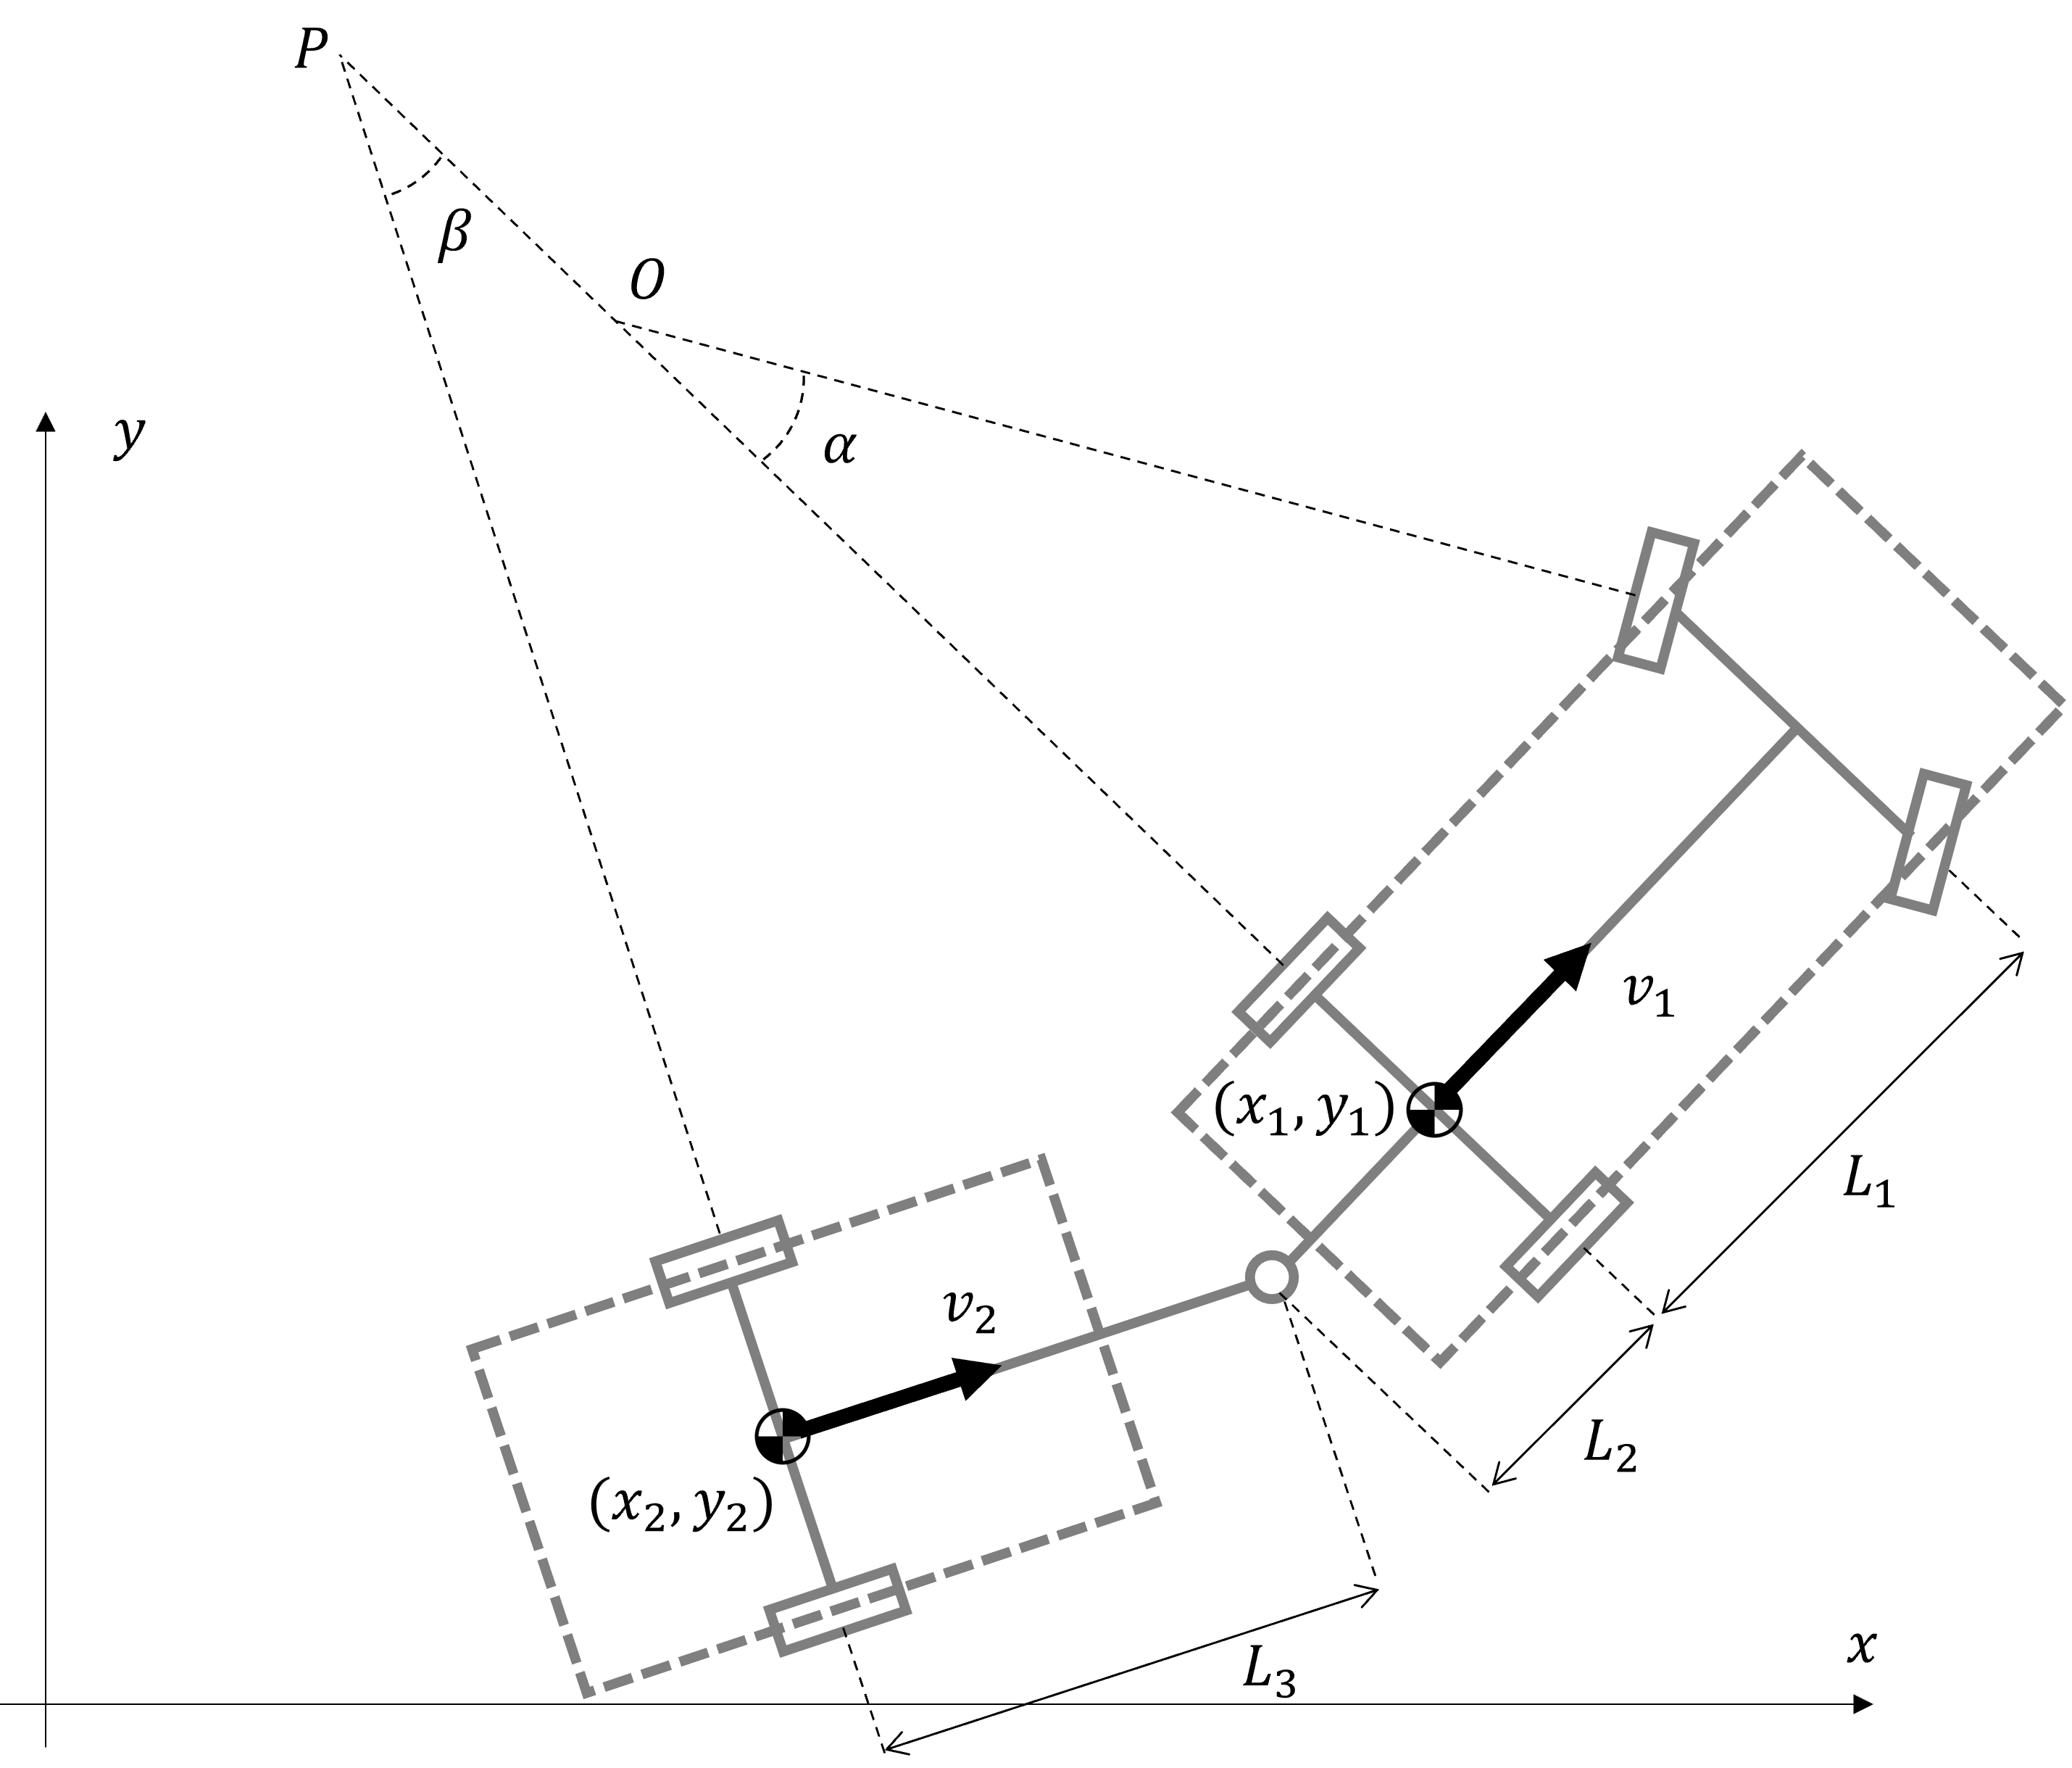
\includegraphics[scale=0.35]{fig/full_track_vehicle_model.png}
\caption{Kinematic full-track model of TTWR}
\label{fig:full track kinematics mdoel}
\end{figure}

This state-space model of TTWR in this paper is illustrated in Figure \ref{fig:full track kinematics mdoel}, where the trailer has a single axle and a conventional overrun braking system. The assumptions for the TTWR system are as summarized as follows: 

\begin{itemize}
  \item The system has a unique pivoting point, known as the hitch, which is essential in yielding the unstable equilibrium point during reverse driving.
  \item The system is defined on a flat surface and without slide slip in the kinematics model and simulation environment.
  \item The trailer has a uniformly distributed mass.
\end{itemize}

Because all the perception values are received in the vehicle coordinate, it is essential to build the reference point coordinate transformation between the vehicle coordinate and the world coordinate. In this paper, only the translation from trailer coordinate to world coordinate is explained, because host coordinate transformation also follows a similar computation.

Under the trailer coordinate, the reference points coordinates can be expressed as:
\begin{equation}
P_2=\left[\begin{array}{cccc}
x_{21} & x_{22} & \cdots & x_{2n} \\
y_{21} & y_{22} & \cdots & y_{2n}
\end{array}\right]
\label{eq: reference point matrix}
\end{equation}
where $P_2$ is the coordinate vector matrix, each column vector of the matrix represents a reference point (e.g. surrounding obstacle detections, trailer corner coordinate and et al.) under the trailer coordinate system. $\left(x_{21}, x_{22}, \ldots, x_{2n}\right)$ and $\left(y_{21}, y_{22}, \ldots, y_{2n}\right)$ are X-coordinate and the Y-coordinate values respectively.

In linear algebra, the rotation matrix $R_\text{world}$ and the translation matrix $T_\text{world}$ can be known as:
\begin{equation}
\operatorname{R}_\text{world} = \left[\begin{array}{ccc}
\cos \theta_2 & -\sin \theta_2 \\
\sin \theta_2 & \cos \theta_2
\end{array}\right]
\label{eq: rotation matrix}
\end{equation}

\begin{equation}
\operatorname{T}_\text{world} =\left[\begin{array}{ccc}
t_{x2} & t_{y2}
\end{array}\right]^T
\label{eq: translation matrix}
\end{equation}
where the $(x_2, y_2)$ are the origin point of the trailer coordinate on the trailer rear axle center, and then the coordinate vector translation from trailer coordinate to world coordinate can be expressed as:
\begin{equation}
P_\text{world}=\operatorname{R}_\text{world} * P_2 + \operatorname{T}_\text{world}
\label{eq: transform coordinate 2 to coordinate world}
\end{equation}

\begin{figure}[h]
\centering
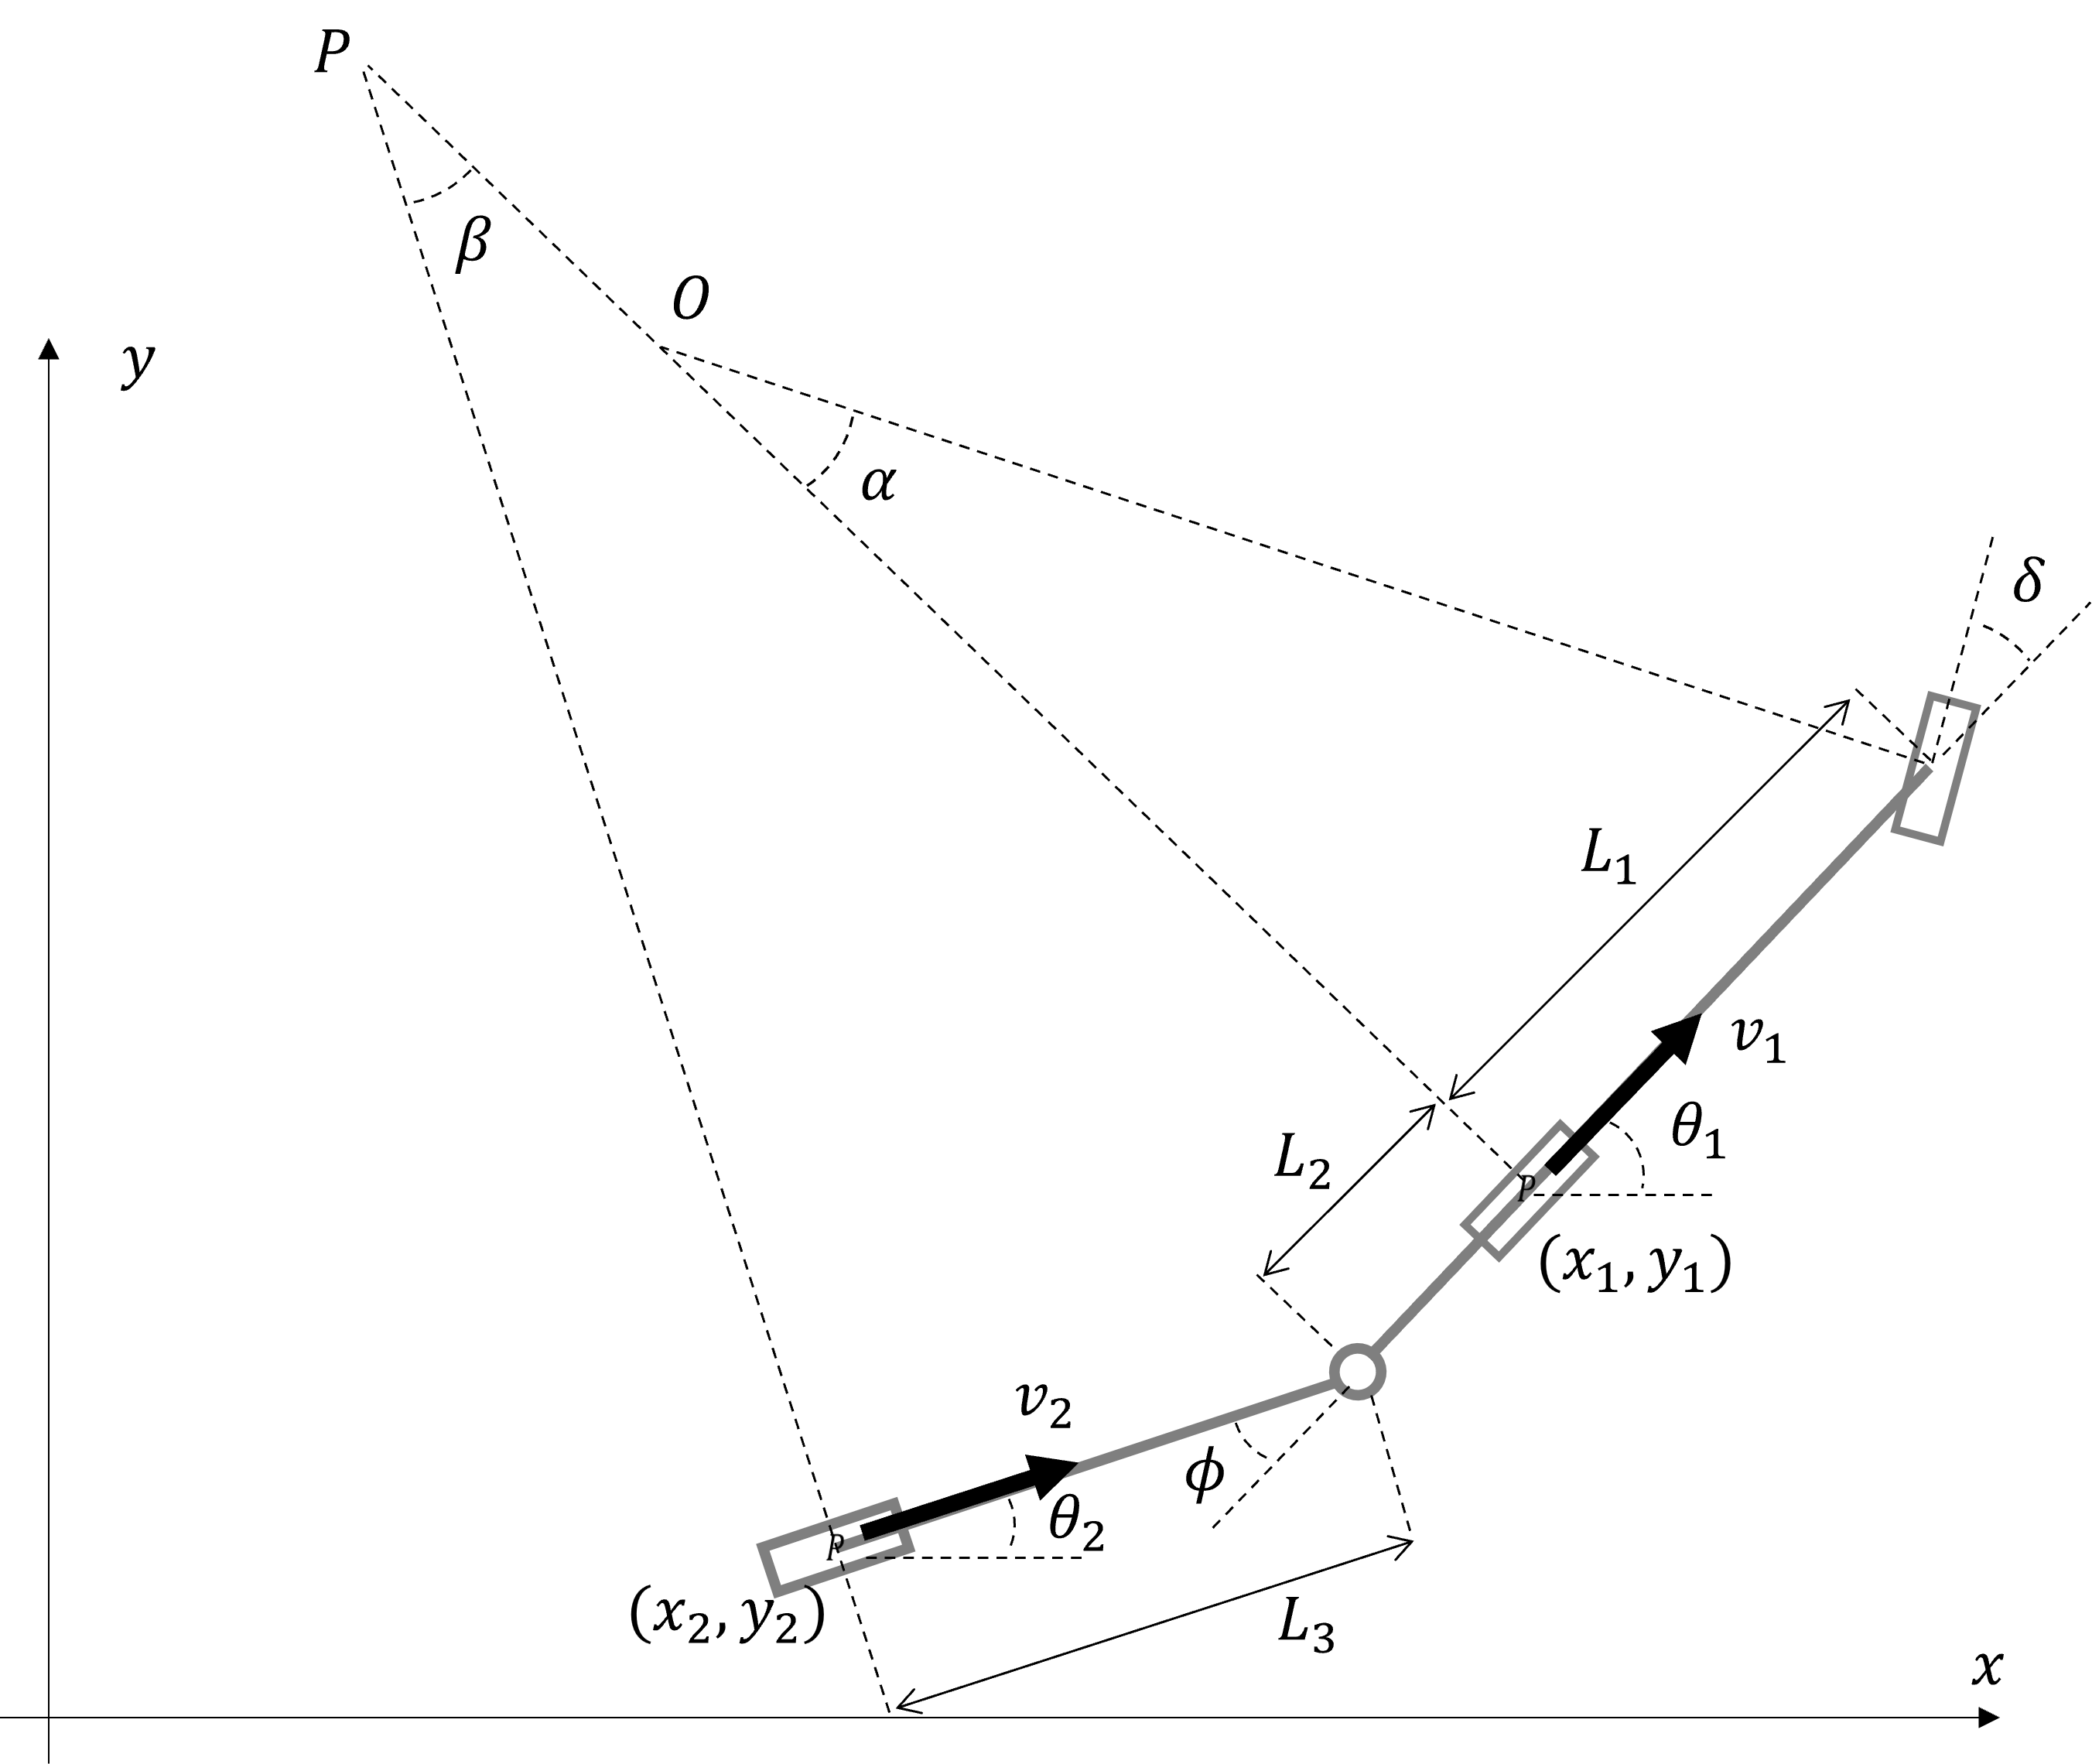
\includegraphics[scale=0.35]{fig/bicycle_vehicle_model.png}
\caption{Simplified bicycle kinematic model of TTWR}
\label{fig:Simplified bicycle kinematic model of TTWR}
\end{figure}

In the world coordinate, the host vehicle state model is referred to as the front wheel Ackerman steering model, which allows control of the front wheel orientation relative to the heading of the vehicle. Due to limitations on the available computational power, vehicle dynamics are often highly simplified at the simulation phase \parencite{polack2017kinematic}. Because the state model in this paper is carried out at low speed and with the assumption of an ideally flat environment, the full track model represented in Figure \ref{fig:full track kinematics mdoel} can be further simplified as the kinematic bicycle model in Figure \ref{fig:Simplified bicycle kinematic model of TTWR}, and the host vehicle kinematic equation can be expressed as:
\begin{equation} \dot{x}_1=v \cos{\theta_1} \label{eq: x1}\end{equation}
\begin{equation} \dot{y}_1=v \sin{\theta_1} \label{eq: y1}\end{equation}
\begin{equation} \dot{\theta}_1 = \frac{v}{L_1}\tan{\delta} \label{eq: theta1}\end{equation}

The kinematic model of the trailer can be derived by propagating the state space of the host vehicle, as the trailer's kinematics are influenced by the maneuver of the host vehicle. The longitudinal speed of the trailer can be estimated by projecting the normal and longitudinal speed of the host vehicle onto the longitudinal axis of the trailer at the hitch point. Following the bicycle kinematic model, the states $[x_2, y_2, \theta_2]^T$ of the trailer can be expressed as:
\begin{equation} \dot{x}_2 = v \cos{\phi} (1 - \frac{L_2}{L_1}\tan{\phi}\tan{\delta})\cos{\theta_2} \label{eq: x2}\end{equation}
\begin{equation} \dot{y}_2 = v \cos{\phi} (1 - \frac{L_2}{L_1}\tan{\phi}\tan{\delta})\sin{\theta_2} \label{eq: y2}\end{equation}
\begin{equation} \dot{\theta}_2 = -v (\frac{\sin{\phi}}{L_3} + \frac{L_2}{L_1 L_3}\cos{\phi}\tan{\delta} ) \label{eq: theta2}\end{equation}

To evaluate the threat of jack-knifing, the host-trailer angle is also required for trailer state prediction, which is defined by the difference between Eqn.\ref{eq: theta2} and Eqn.\ref{eq: theta1}:
\begin{equation} 
\dot{\phi} = -\frac{v}{L_3}\sin{\phi} - \frac{v}{L_1} ( 1 + \frac{L_2 \cos{\phi}}{L_3}) \tan{\delta} 
\label{eq: phi}
\end{equation}

During reverse driving, the host-trailer system is limited to one degree of freedom in control, which is the host vehicle steering input, the system control is designed to minimize mainly the trailer's tracking error. So, the control reference variables are defined by the trailer’s rear axle center position $(x_2, y_2)$, and heading ${\theta}_2$ compared with the parking slot's reference position  $(x_{goal}, y_{goal})$, and heading angle ${\theta}_{goal}$.

\section{TTWR system physical constrains}

Jack-knifing is a significant constrain in the dynamics of truck trailer wheeled robot systems. It occurs when the angle between the truck and trailer reaches a point where control over the trailer's direction is lost during reverse motion. Rather than aligning with the desired trajectory, the angle continues to grow, culminating in the trailer contacting the tractor. At this stage, the system enters an uncontrollable state, representing a critical failure mode in the control of tractor-trailer systems. Abraham \parencite{abraham2013trailer} provides an explanation for the phenomenon of jack-knifing, identifying it as a situation where the trailer's angular velocity surpasses that of the towing vehicle, even when maximum steering input is applied. Geometrically, this is interpreted as the trailer's center of rotation moving beyond the corresponding point of the towing vehicle. The critical threshold for jack-knifing is reached when these two centers of rotation coincide, leading to a loss of control over the trailer's direction.

\section{Controllability}

Controllability is an important characteristic for the control system, which significantly impacts various control challenges, including stabilizing unstable systems through feedback and optimizing control. Complete state controllability refers to the capacity of an external input (consisting of control variables) to move the system's internal states from any starting states to any final states within a finite time frame. In simpler terms, a system is considered controllable if there exists a control input that enables the transition from any initial state to any desired final state within a specified time interval.

Consider the continuous linear system
\begin{equation}
\label{eqn: lti system states}
\begin{aligned}
& \dot{{x}}(t)=A(t) {x}(t)+B(t) {u}(t) \\
& {y}(t)=C(t) {x}(t)+D(t) {u}(t) .
\end{aligned}
\end{equation}
where ${x}(t_0)=x^0$ is the initial states when the system starts.

The state pair sets $(x, u)$ which solve Equation \ref{eqn: lti system states} for by setting the initial states $\left(t_0, x^0\right)$ is called the behaviour $\mathcal{B}_{(A, B)}$ of Equation \ref{eqn: lti system states}:
\begin{equation}
\mathcal{B}_{(A, B)}:=\left\{(x, u) \in X \times U \mid \exists\left(t_0, x^0\right) \in \mathbb{R} \times \mathbb{R}^n, \quad x(\cdot)=x\left(\cdot ; t_0, x^0, u\right)\right\}
\end{equation}

Here, $X$ is a suitable space of functions such that
\begin{equation}
\left\{x\left(\cdot ; t_0, x^0, u\right) \mid\left(t_0, x^0\right) \in \mathbb{R} \times \mathbb{R}^n, \quad u \in U\right\} \subseteq X .
\end{equation}

Regarding the concept of controllability, the system $(A, B)$ is called 
\begin{itemize}
    \item Reachable at time $T>0$ if for all $x^1 \in \mathbb{R}^n$ there exists $(x, u) \in \mathcal{B}_{(A, B)}$ such that $x(0)=0$ and $x(T)=x^1$,
    \item Controllable at time $T$ if for all $x^0, x^1 \in \mathbb{R}^n$ there exists $(x, u) \in \mathcal{B}_{(A, B)}$ such that $x(0)=x^0$ and $x(T)=x^1$,
    \item Null-controllable at time $T$ if for all $x^0 \in \mathbb{R}^n$ there exists $(x, u) \in \mathcal{B}_{(A, B)}$ such that $x(0)=x^0$ and $x(T)=0$.
\end{itemize}

To determine which states can be more or less easily controlled, it is required to examine the eigen decomposition of the Controllability Gramian. This process reveals insights into the relationships between the system states and how they respond to the control inputs. The Controllability Gramian $W\left(t_0, t_1\right)$ is defined as:
\begin{equation}
\label{eqn_controllability_gramian}
W\left(t_0, t_1\right)=\int_{t_0}^{t_1} \phi\left(t_0, t\right) B(t) B(t)^T \phi\left(t_0, t\right)^T d t
\end{equation}
where $\phi$ is the state-transition matrix. 

The Equation \ref{eqn_controllability_gramian} means if there exists a control $u$ from state $x_0$ at time $t_0$ to state $x_1$ at time $t_1>t_0$ if and only if $x_1-\phi\left(t_0, t_1\right) x_0$ is in the column space of the Controllability Gramian.

In fact, if $\eta_0$ is a solution to $W\left(t_0, t_1\right) \eta=x_1-\phi\left(t_0, t_1\right) x_0$ then a control given by $u(t)=-B(t)^T \phi\left(t_0, t\right)^T \eta_0$ would make the desired transfer.

Note that the matrix $W$ defined as above has the following properties:
\begin{itemize}
\item  $W\left(t_0, t_1\right)$ is symmetric
\item $W\left(t_0, t_1\right)$ is positive semidefinite for $t_1 \geq t_0$
\item $W\left(t_0, t_1\right)$ satisfies the linear matrix differential equation
\begin{equation}
\frac{d}{d t} W\left(t, t_1\right)=A(t) W\left(t, t_1\right)+W\left(t, t_1\right) A(t)^T-B(t) B(t)^T, W\left(t_1, t_1\right)=0
\end{equation}
\item $W\left(t_0, t_1\right)$ satisfies the equation \parencite{brockett2015finite}
\begin{equation}
W\left(t_0, t_1\right)=W\left(t_0, t\right)+\phi\left(t_0, t\right) W\left(t, t_1\right) \phi\left(t_0, t\right)^{T}
\end{equation}
\end{itemize}

Gramians are also useful to determine the minimum-energy control ${u}(t)$ required to navigate the system to ${x}\left(t_f\right)$ at time $t_f$ from ${x}(0)=0$ \parencite{brunton2022data}:
\begin{equation}
{u}(t)={B}^*\left(e^{{A}\left(t_f-t\right)}\right)^* {W}_c\left(t_f\right)^{-1} {x}\left(t_f\right) .
\end{equation}

The total energy expended by this control law is given by
\begin{equation}
\int_0^{t_f}\|{u}(\tau)\|^2 d \tau={x}^* {W}_c\left(t_f\right)^{-1} {x} .
\end{equation}

If the controllability matrix is close to singular, more actuation enger will be required to drive the states to certian direction. On the other hand, if the eigenvalues of ${W}_c$ are all large, then the system is easily controlled.

It is generally impractical to compute the Gramians directly using Equation \ref{eqn_controllability_gramian}. Instead, the Controllablity Gramian is the solution to the following Lyapunov equation:
\begin{equation}
{A W}_c+{W}_c {A}^*+{B B}^*={0},
\end{equation}
while the observability Gramian is the solution to
\begin{equation}
{A}^* {W}_o+{W}_o {A}+{C}^* {C}={0} .
\end{equation}

Obtaining Gramians by solving a Lyapunov equation is typically quite expensive for high-dimensional systems. Instead of this computationally demanding approach, Gramians are frequently approximated empirically. This approximation is achieved using snapshot data gathered from both the direct system and the adjoint system, providing a more efficient means to estimate these important mathematical constructs.

In practice, the Controllability Gramian requires the integration of a system's state-transition matrix. For a simpler assessment of system controllability, a rank condition can be used that is similar to the Kalman rank condition found in time-invariant systems, which shows that the Controllability of a LTI system is determined entirely by the column space of the controllability matrix $\mathcal{C}$ :
\begin{equation}
\mathcal{C}=\left[\begin{array}{lllll}
{B} & {AB} & {A}^2 {~B} & \cdots & {A}^{n-1} {~B}
\end{array}\right] .
\end{equation}

If the matrix $\mathcal{C}$ has $n$ linearly independent columns, meaning that it spans all of $\mathbb{R}^n$, then the system is considered controllable. The span of the columns of the controllability matrix$\mathcal{C}$ forms a Krylov subspace, which identifies the directions in $\mathbb{R}^n$ that can be manipulated with control. Consequently, controllability not only implies the possibility of arbitrary eigenvalue placement but also ensures that any state $\xi \in \mathbb{R}^n$  can be reached within a finite time using a specific actuation signal ${u}(t)$ \parencite{brunton2022data}.

In general, for a system $(A, B)$ the following statements are equivalent:
\begin{itemize}
    \item There exists $T>0$ such that $(A, B)$ is controllable at time $T$.
    \item $\operatorname{im}(K(A, B))=\mathbb{R}^n$
    \item $\operatorname{rank}(K(A, B))=n$
    \item For all $T>0$ the system $(A, B)$ is controllable at time $T$. We say that $(A, B)$ is controllable.
\end{itemize}

\section{TTWR system analysis}
\label{section: ttwr system analysis}

To identify the properties and conditions of the truck trailer system, its equilibrium, observability, and controllability are analyzed. Let $ x = [y_2, \theta_2, \phi]^\intercal$ be the trailer states obtained from Equation \ref{eq: x2} - \ref{eq: theta2} by neglecting the longitudinal component $x_3$, the state space model can be written as \parencite{altafini2001feedback}:

\begin{equation} \dot{x} = v ( \mathcal{A} ( x ) + \mathcal{B} (x;\delta)) \label{eq: state space model}\end{equation}

The equilibrium state of $x$ is the origin $x_e = 0$, and we can derive the trailer equilibrium state from Equation \ref{eq: phi}: 

\begin{equation} x_e = \{(y_2, \theta_2, \phi) \mid \delta = 0, y_2 \in \mathbb{R}, \theta_2 \in [-\pi, \pi), \phi = 0\} \label{eq: equilibrium states}\end{equation}

The equilibrium set indicates during reverse driving, the trailer system is in an equilibrium state when the host vehicle and trailer are aligned in either direction, and there should be no steering angle input given by the host vehicle.

To examine the internal asymptotic stability, we substitute $\delta = 0$ into Equation 8, resulting in the following equation:
\begin{equation} 
\dot{x} = v ( \mathcal{A} x + \mathcal{B} \delta)
\label{eq: state space when delta is 0}
\end{equation}
where
\begin{equation} 
\mathcal{A} = \begin{bmatrix}
0 & 1 & 0 \\
0 & 0 & -\frac{1}{L_3} \\
0 & 0 & -\frac{1}{L_3}
\end{bmatrix} 
\mathcal{B}= \begin{bmatrix}
0 \\
\frac{L_2}{L_1L_3} \\
-\frac{L_3+L_2}{L_1L_3}
\end{bmatrix} \label{eq: state transfer matrix linearization}\end{equation}

By using the Cayley-Hamilton theorem, the controllability matrix $\mathcal{C} = [B, AB, AAB]$ is row full rank for state space in Equation \ref{eq: state space when delta is 0}, which shows the host-trailer system to be controllable out of the singular locus \parencite{altafini1999controllability}, and the origin of the nonlinear system can be made an asymptotically stable equilibrium by state feedback.


\begin{figure}
     \centering
     \begin{subfigure}[b]{0.8\textwidth}
         \centering
         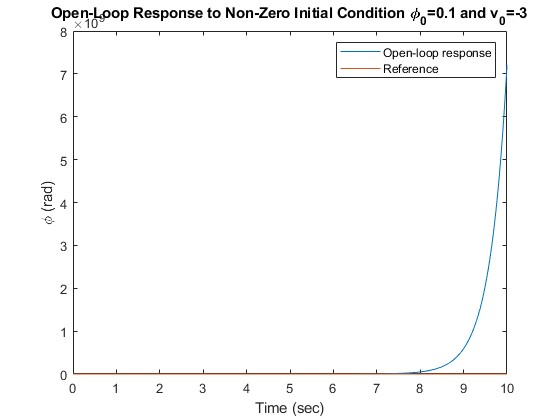
\includegraphics[width=0.7\linewidth]{fig/openloop_respond/negative velo openloop response - Copy.jpg}
         \caption{The positive velocity indicates stable system behaviour when teh TTWR can correct its $\Phi$ value}
     \end{subfigure}
     \vfill 
     \begin{subfigure}[b]{0.8\textwidth}
         \centering
         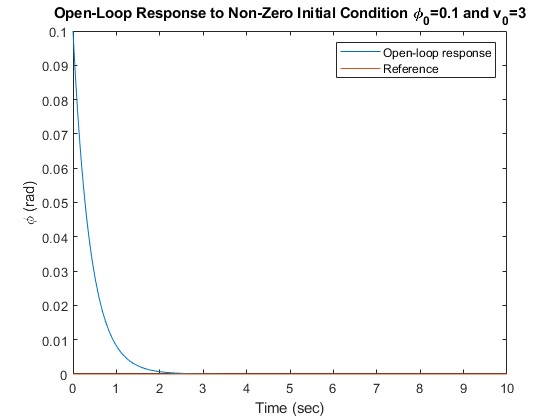
\includegraphics[width=0.7\linewidth]{fig/openloop_respond/positive velo openloop response - Copy.jpg}
         \caption{The negative velocity will cause unstable system performance, the $\Phi$ angle keeps increasing until reach jacknifing}
     \end{subfigure}
    \caption{Open loop respond comparison between the positive and negative truck velocity}
\end{figure}

% Chapter 5
\chapter{\leavevmode\newline Classical TTWR reverse parking control system}
\chaptermark{Heading on Chapter Pages}
\label{chap:Chapter_5}

In the first stage of this research, a traditional hierarchical control system has been developed as a baseline for the future benchmark testing, by using Dubins path planning and the LQR controller. This section introduces details of this implementation for the TTWR reverse parking control. The usage of Dubins path planning ensures a minimal turning radius limitation, providing a smooth and efficient trajectory for the TTWR. Coupled with this, the LQR controller optimizes steering responses for the path following. Together, these methodologies not only streamline the reverse driving process but also enhance the precision and reliability of the control system, ensuring optimal performance in real-world scenarios.

\section{Dubin path planning}
The Dubins path, designed with a consistent velocity, operates with a singular control variable: its steering. The Dubins path is constructed by establishing common tangents between two circular arcs. These tangents can either connect the arcs from the outside (external tangents), or they can intersect the arcs diagonally, termed as internal tangents. This section will primarily focus on the Dubins path construction using an external tangent. The methodology for the internal tangent follows a similar logic. Figure \ref{fig:dubins_example} showed the geometric construction of the Dubins path. The dubins path has three distinct states: maximum right turn (R), maximum left turn (L), and straight (S). Previous research from Dubins \parencite{dubins1957curves} has shown that optimal trajectory between two points with certain direction can be represented using six specific control sequences: RSR, RSL, RLR, LSL, LSR, and LRL. For simplification, the curvatures resulting from R and L can be labeled as C, leading to sequences like CSC and CCC. 

\begin{figure}[h]
\centering
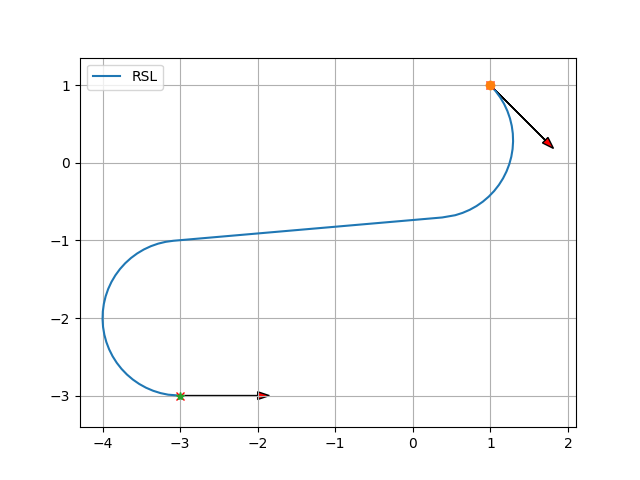
\includegraphics[width=0.8\textwidth]{fig/dubins/dubins_example.png}
\caption{Dubins path starting from point (1, 1) with heading angle $\frac{-\pi}{4}$ and ending at (-3, -3) with heading angle 0}
\label{fig:dubins_example}
\end{figure}

\subsection{CSC Dubins Path}

The CSC trajectories include RSR, LSR, RSL, and LSR, which stands for a turn followed by a straight line followed by another turn (Shown in Figure \ref{fig:dubins pattern CSC}).

Pick a position and orientation for your start and goal configurations. Draw your start and goal configurations as points in the plane with arrows extending out in the direction the car is facing. Next, draw circles to the left and right of the car with radius $r_{min}$ . The circles should be tangent at the location of the car. Draw tangent lines from the circles at the starting configuration to the circles at the goal configuration. In the next section I’ll discuss how to compute this, but for now just draw them.

For every pair of circles, whether it's RR, LL, RL, or LR, four potential tangent lines can be drawn. However, only one of these lines for each pair is valid. Specifically, for the RR circles, a single line drawn from the agent's circle intersects the goal's circle in a manner that ensures the correct direction, whose Dubins trajectory can be simplified as RR without S in between. As a result, for any CSC Trajectory, there exists a distinct tangent line to be followed. This line represents the 'S' segment of the trajectory. The points where this line touches the circles are the critical points the agent needs to navigate through to complete its path. Essentially, determining these trajectories hinges on accurately identifying these tangent points.

\begin{figure}
     \centering
     \begin{subfigure}[b]{0.2\textwidth}
         \centering
         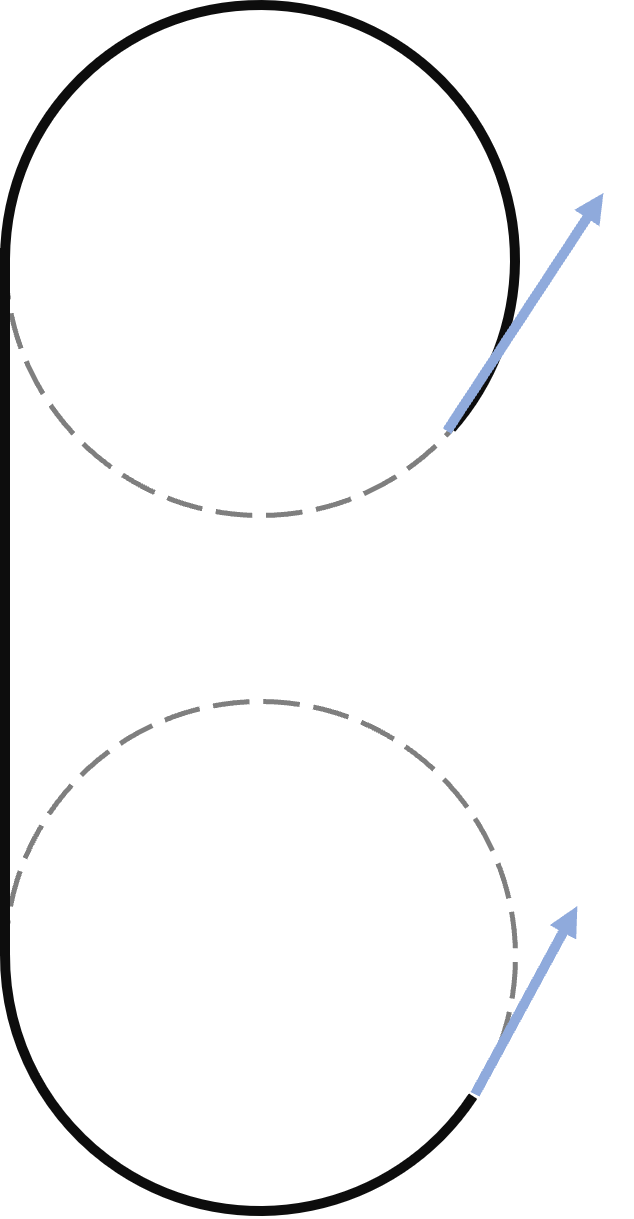
\includegraphics[scale=0.7]{fig/dubins/LSL.png}
         \caption{dubins pattern LSL}
         \label{fig: dubins pattern LSL}
     \end{subfigure}
     \hfill
     \begin{subfigure}[b]{0.2\textwidth}
         \centering
         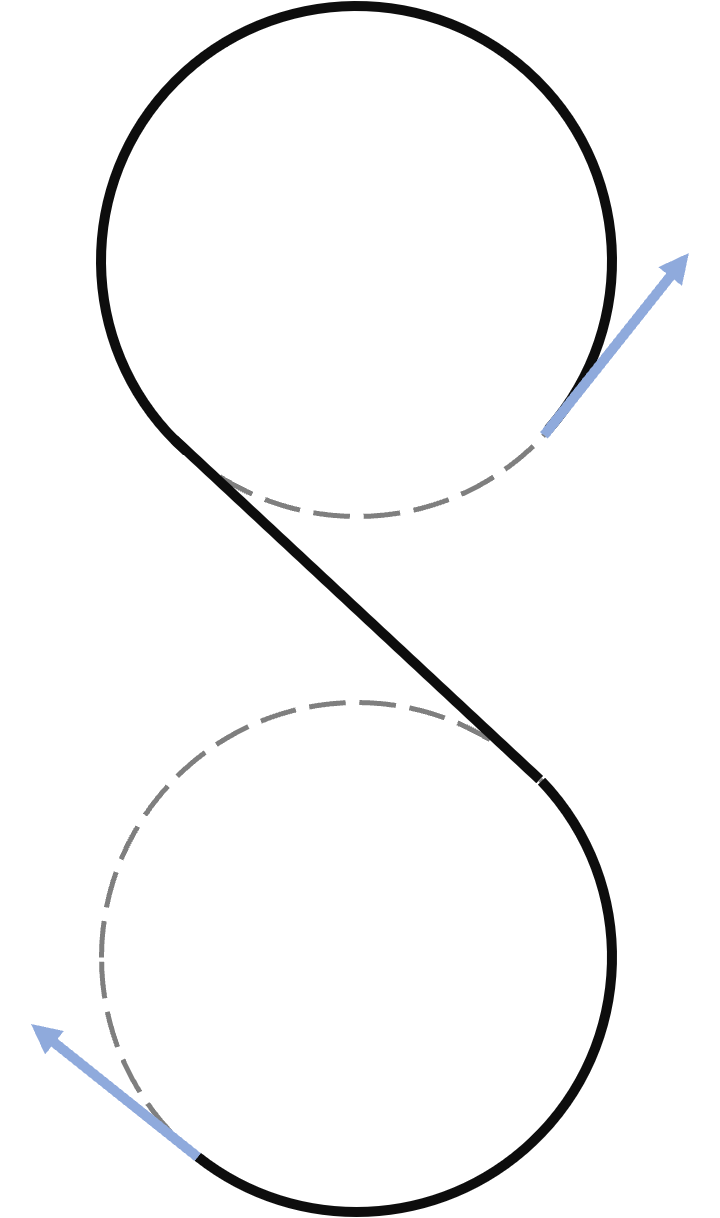
\includegraphics[scale=0.7]{fig/dubins/LSR.png}
         \caption{dubins pattern LSR}
         \label{fig:dubins pattern LSR}
     \end{subfigure}
     \hfill
     \begin{subfigure}[b]{0.2\textwidth}
         \centering
         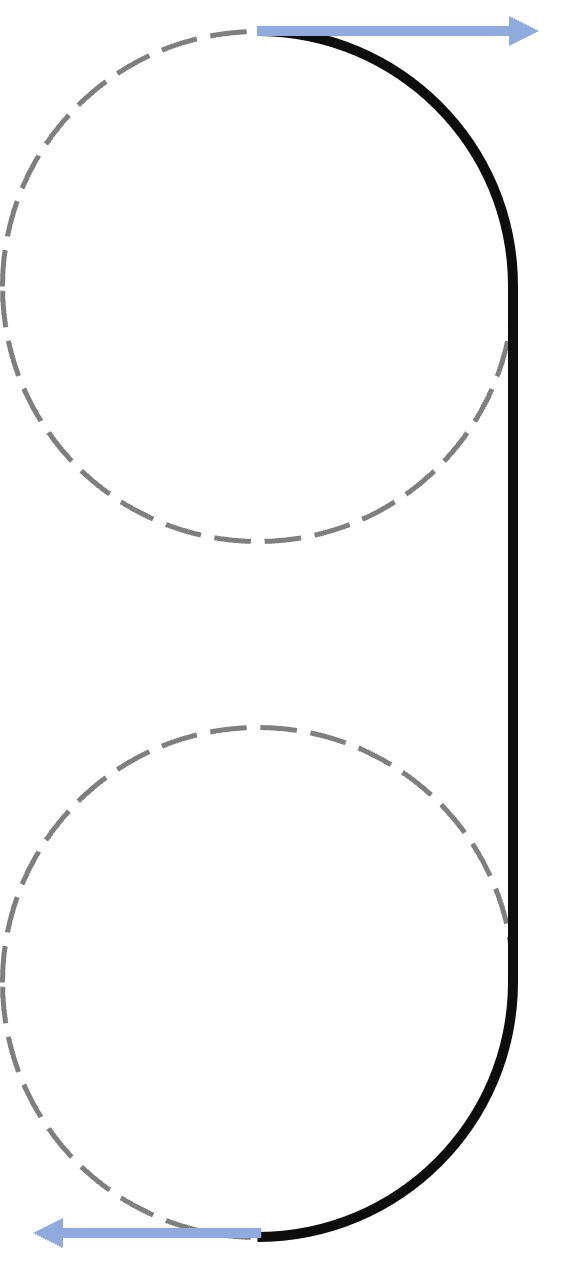
\includegraphics[scale=0.7]{fig/dubins/RSR.png}
         \caption{dubins pattern RSR}
         \label{fig:dubins pattern RSR}
     \end{subfigure}
     \hfill
     \begin{subfigure}[b]{0.2\textwidth}
         \centering
         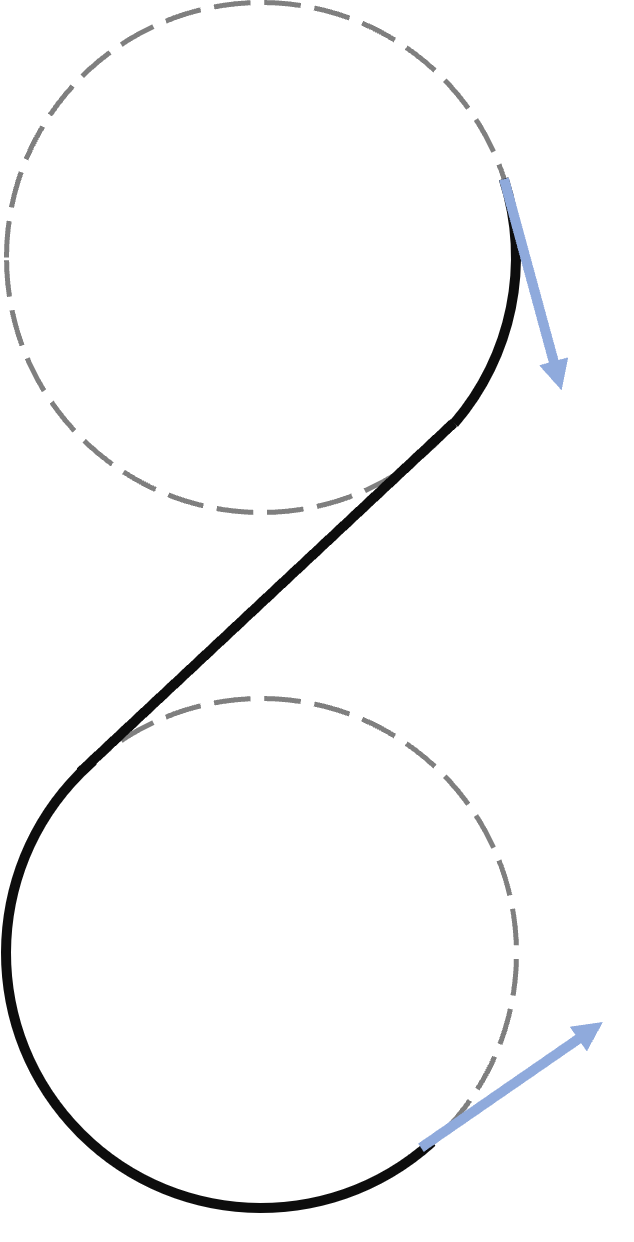
\includegraphics[scale=0.7]{fig/dubins/RSL.png}
         \caption{dubins pattern RSL}
         \label{fig:dubins pattern RSL}
     \end{subfigure}
        \caption{Four patterns under CSC type }
        \label{fig:dubins pattern CSC}
\end{figure}

\subsection{CCC Dubins path}

The CCC trajectories is different from CSC in the connection path, which only involve an initial turn, followed by a turn in the opposite direction, and then revert to the initial turning direction, as exemplified by the RLR Trajectory in Figure \ref{fig:dubins pattern CCC}. These trajectories are applicable when the ego vehicle and the target position are close within a threshold. If they aren't, one of the circles would necessitate a radius exceeding $r_{min}$ . In such cases, the CCC Trajectory becomes less than ideal. For the Dubin's path planning, there are only two types of CCC trajectories: RLR and LRL. Simply determining the tangent lines between RR or LL circles isn't sufficient in this context. The third circle between the starting and finishing circle in the trajectory remains tangent to both the starting and finishing turning circles. However, the points of tangent differ from those derived from standard tangent line computations. 

\begin{figure}
     \centering
     \begin{subfigure}[b]{0.4\textwidth}
         \centering
         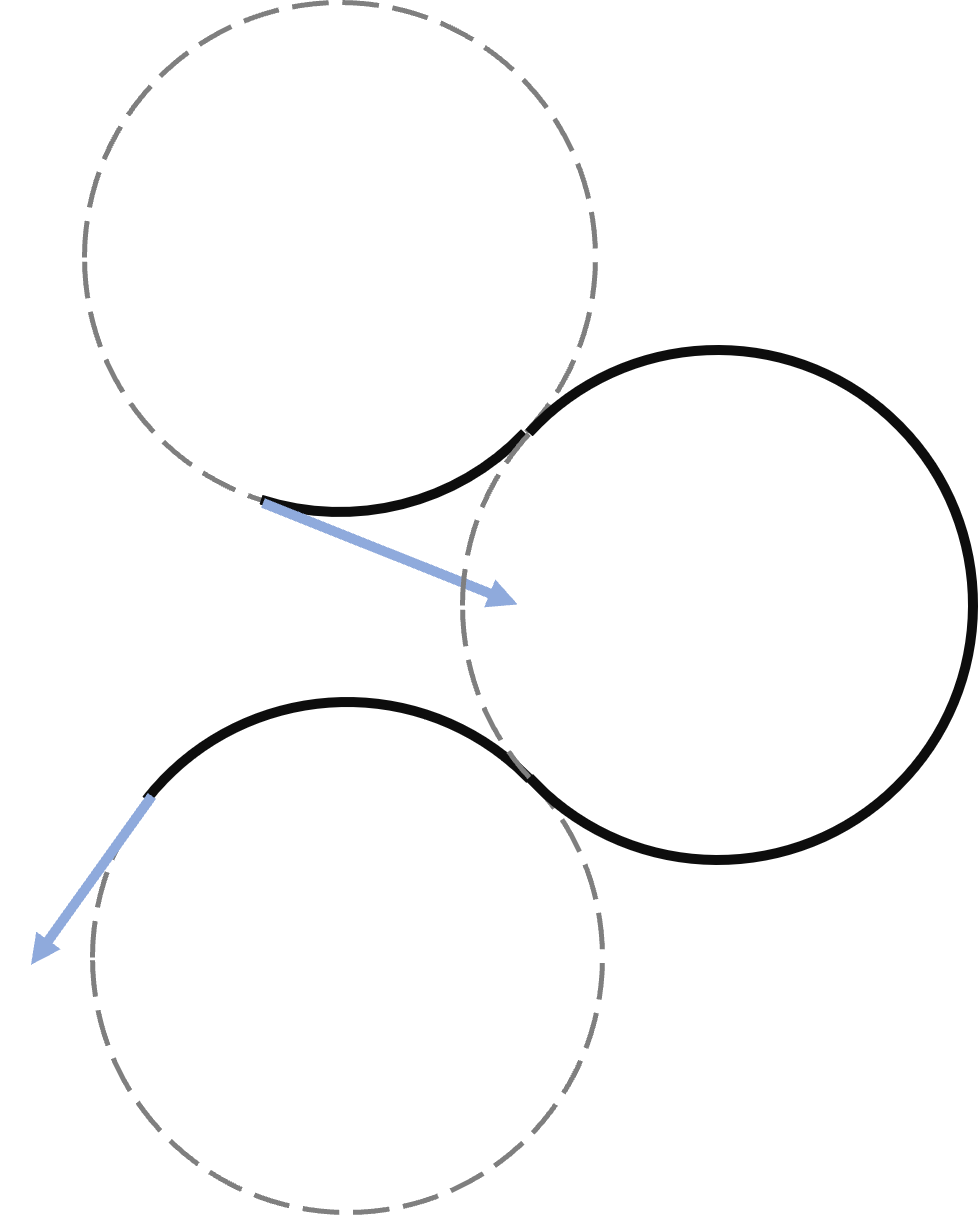
\includegraphics[scale=0.7]{fig/dubins/LRL.png}
         \caption{dubins pattern LRL}
         \label{fig: dubins pattern LRL}
     \end{subfigure}
     \hfill
     \begin{subfigure}[b]{0.4\textwidth}
         \centering
         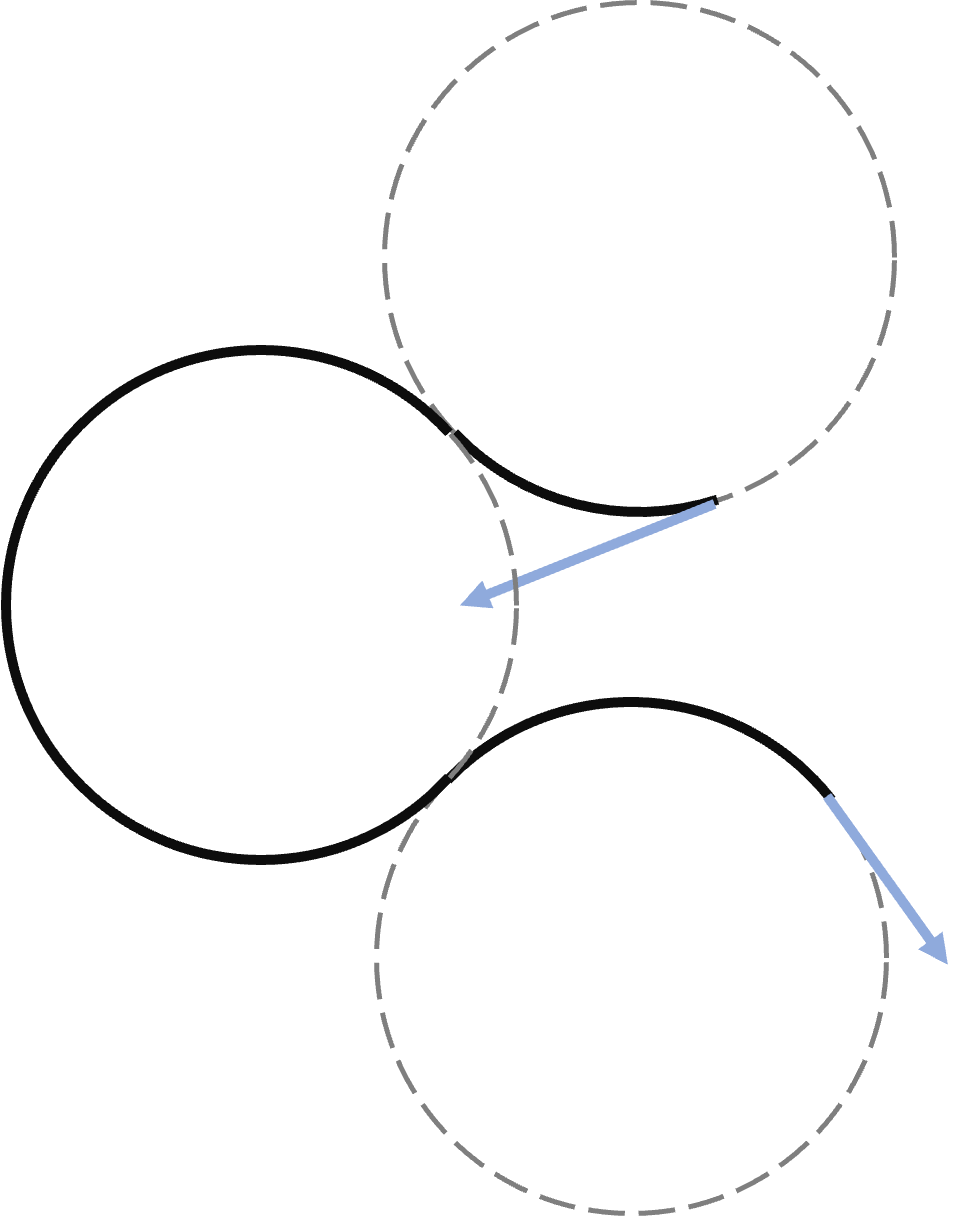
\includegraphics[scale=0.7]{fig/dubins/RLR.png}
         \caption{dubins pattern RLR}
         \label{fig:dubins pattern RLR}
     \end{subfigure}
        \caption{Four patterns under CCC type }
        \label{fig:dubins pattern CCC}
\end{figure}


\subsection{Construction of Dubins path}

Consider the following input parameters.
\begin{enumerate}
\item Initial pose of the target: $P_s\left(x_s, y_s, \theta_s\right)$
\item Final pose of the target: $P_f\left(x_f, y_f, \theta_f\right)$
\item Initial turning radius: $\rho_s\left(=\frac{1}{\kappa_s}\right)$
\item Final turning radius: $\rho_f\left(=\frac{1}{\kappa_f}\right)$
\end{enumerate}
where the initial turning radisu and final turning radius is equal for vehicle path planning, which is determined by vehicle steering angle:
\begin{equation}
    R = \frac{L}{tan(\delta)}
\label{eq: turning radius using delta}
\end{equation}

To compute the Dubins path, we need to start from the two turning circle center $O_s\left(x_{c s}, y_{c s}\right)$ and $O_f\left(x_{c f}, y_{c f}\right)$, which can be computed as:
\begin{align}
    &\left(x_{c s}, y_{c s}\right)=\\ \notag
        &(x_s \pm \rho_s \cos \left(\theta_s \pm \frac{\pi}{2}\right), y_s \pm \rho_s \sin \left(\theta_s \pm \frac{\pi}{2}\right)) 
\end{align}
\begin{align}
        &\left(x_{c f}, y_{c f}\right)=\\ \notag
        &(x_f \pm \rho_f \cos \left(\theta_f \pm \frac{\pi}{2}\right), y_f \pm \rho_f \sin \left(\theta_f \pm \frac{\pi}{2}\right))
\end{align}

Then, the reference circle of radius $\left|\rho_f-\rho_s\right|$ is constructed at $O_f$ for $\rho_s \leq \rho_f$, and the two primary circle center is connected with center reference line:
\begin{equation}
    |c|=\sqrt{\left(x_{c s}-x_{c f}\right)^2+\left(y_{c s}-y_{c f}\right)^2}
\end{equation}

A perpendicular line to $c$ at $O_f$ intersects the reference circle at a point $T^{\prime}$ and the primary circle $C_f$ at the tangent entry point $T_{ent}$. A line from $O_s$ to $T^{\prime}$ is drawn, and another line parallel to $O_f T_{ent}$ is extended from $O_s$ to meet $C_s$ at the tangent exit point $T_{ext}$. The path is completed by connecting the starting position $P_s$ to $T_{ext}$ with an arc of radius $\rho_s$, and from $T_{ent}$ to the finishing position $P_f$ with an arc of radius $\rho_f$. The resulting composite path consists of the starting arc $P_s T_{ext}$, the external tangent line $T_{ext} T_{ent}$, and the ending arc $T_{ent} P_f$. To determine the shortest Dubins path between the same initial and final points, multiple patterns are considered in Figure \ref{fig:dubins pattern difference for same condition}, and the one with the least total length is selected.

\begin{figure}
     \centering
     \begin{subfigure}[b]{0.8\textwidth}
         \centering
         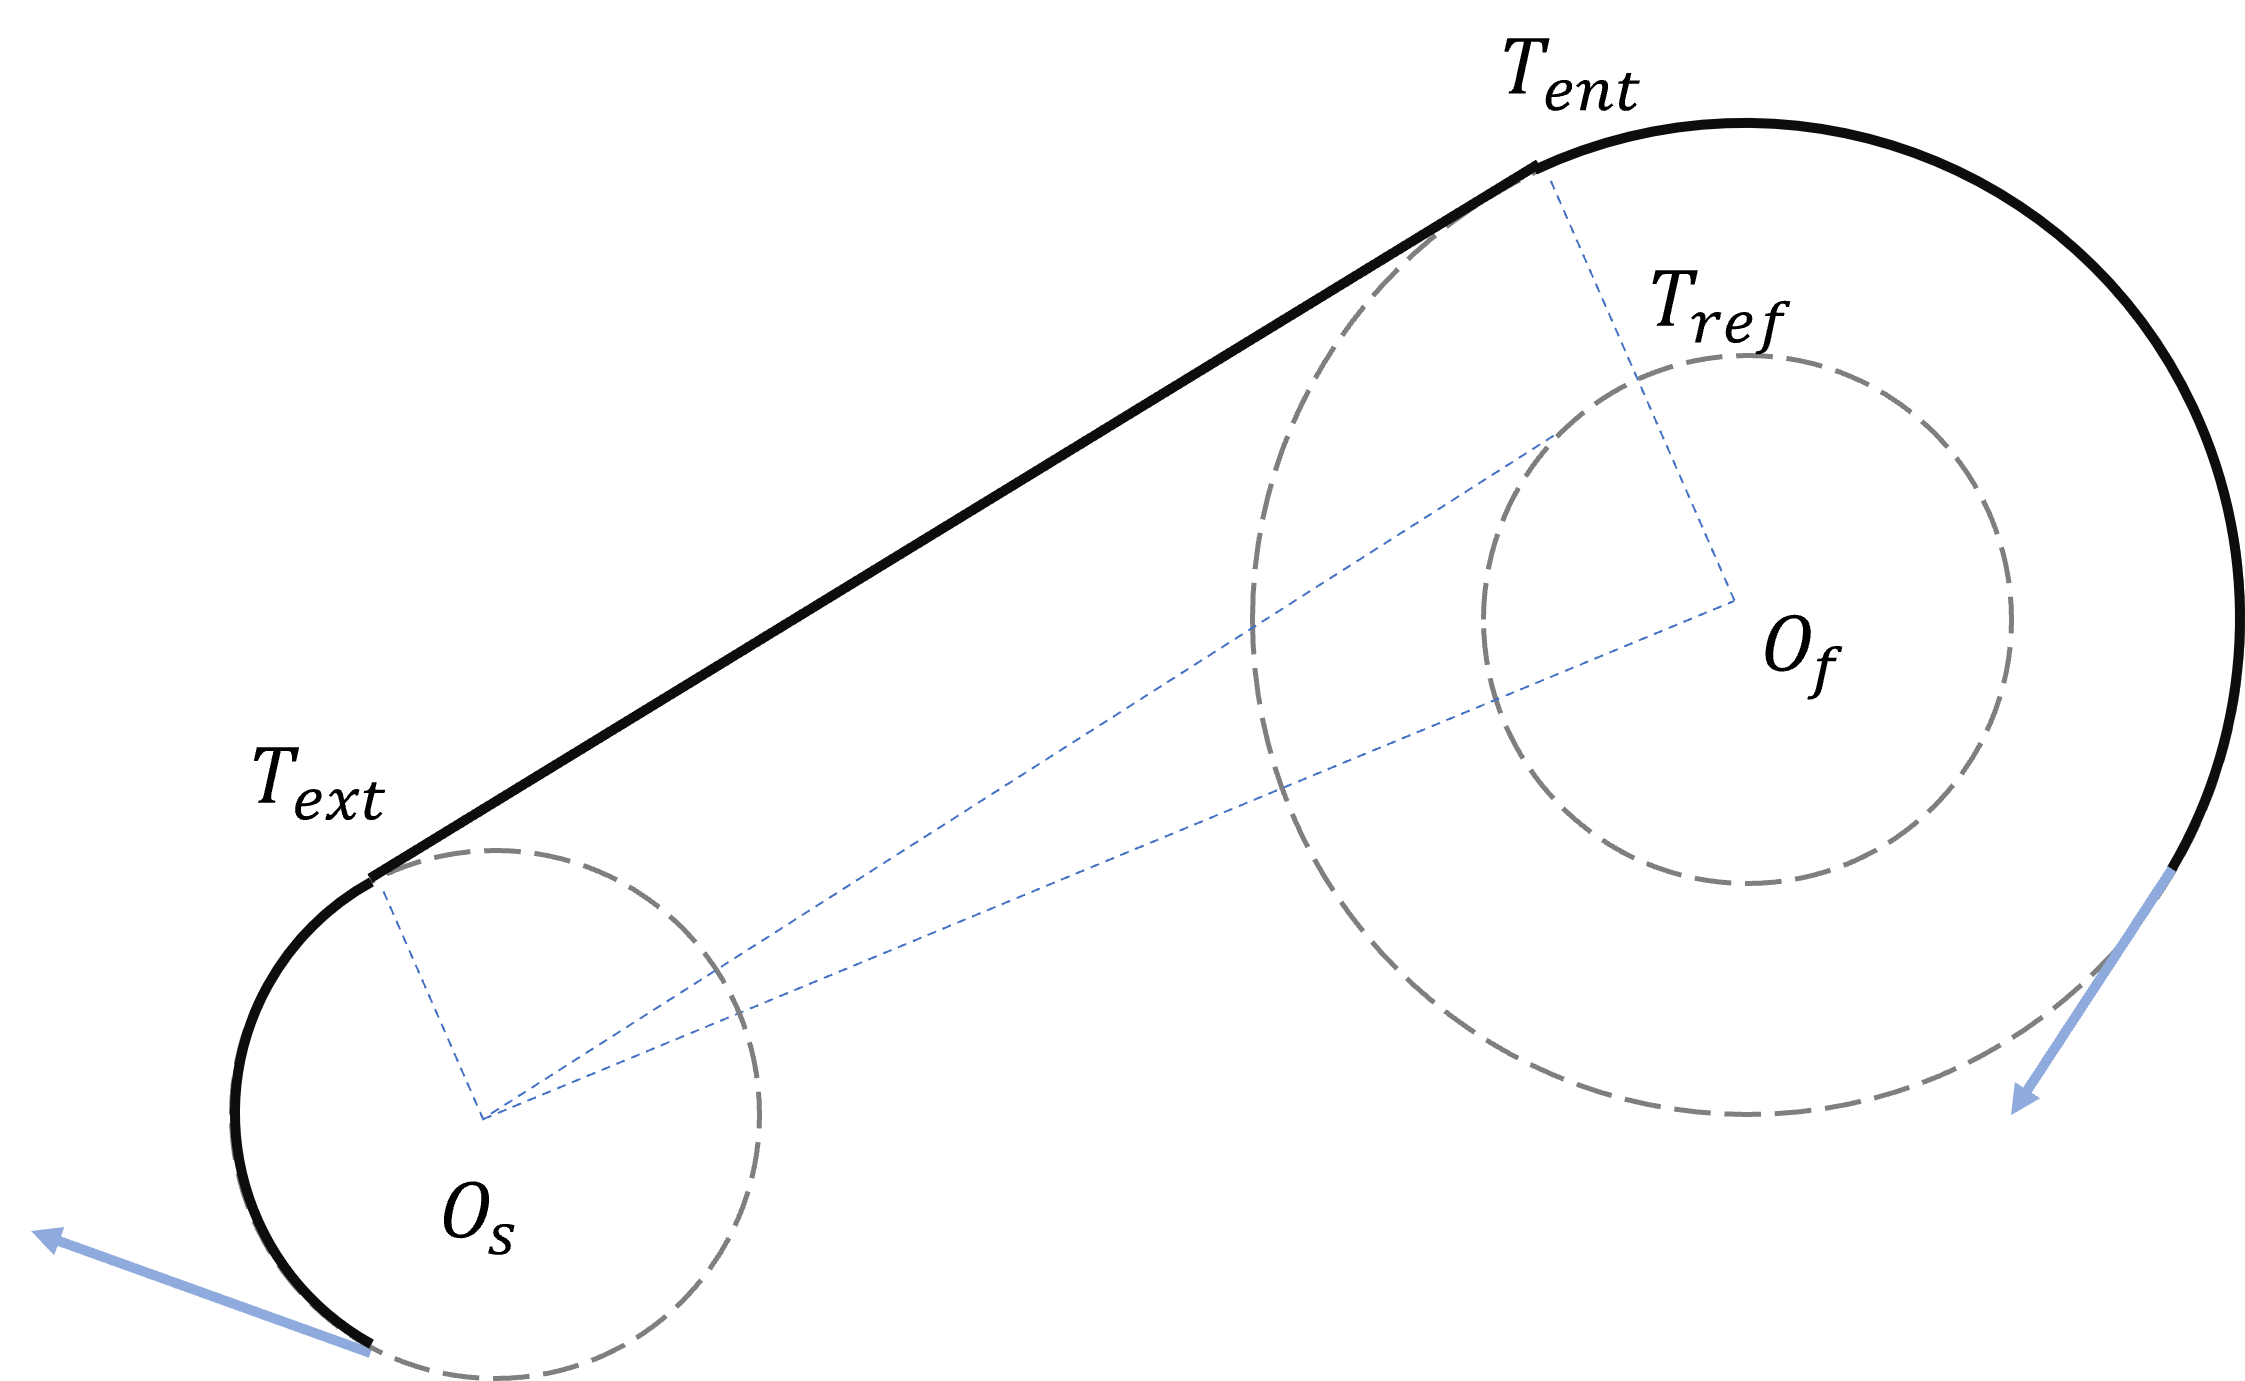
\includegraphics[width=0.7\linewidth]{fig/dubins/dubins_construction_rsr.png}
         \caption{Dubins construction following RSR pattern}
         \label{fig: dubins pattern consturction RSR}
     \end{subfigure}
     \vfill 
     \begin{subfigure}[b]{0.8\textwidth}
         \centering
         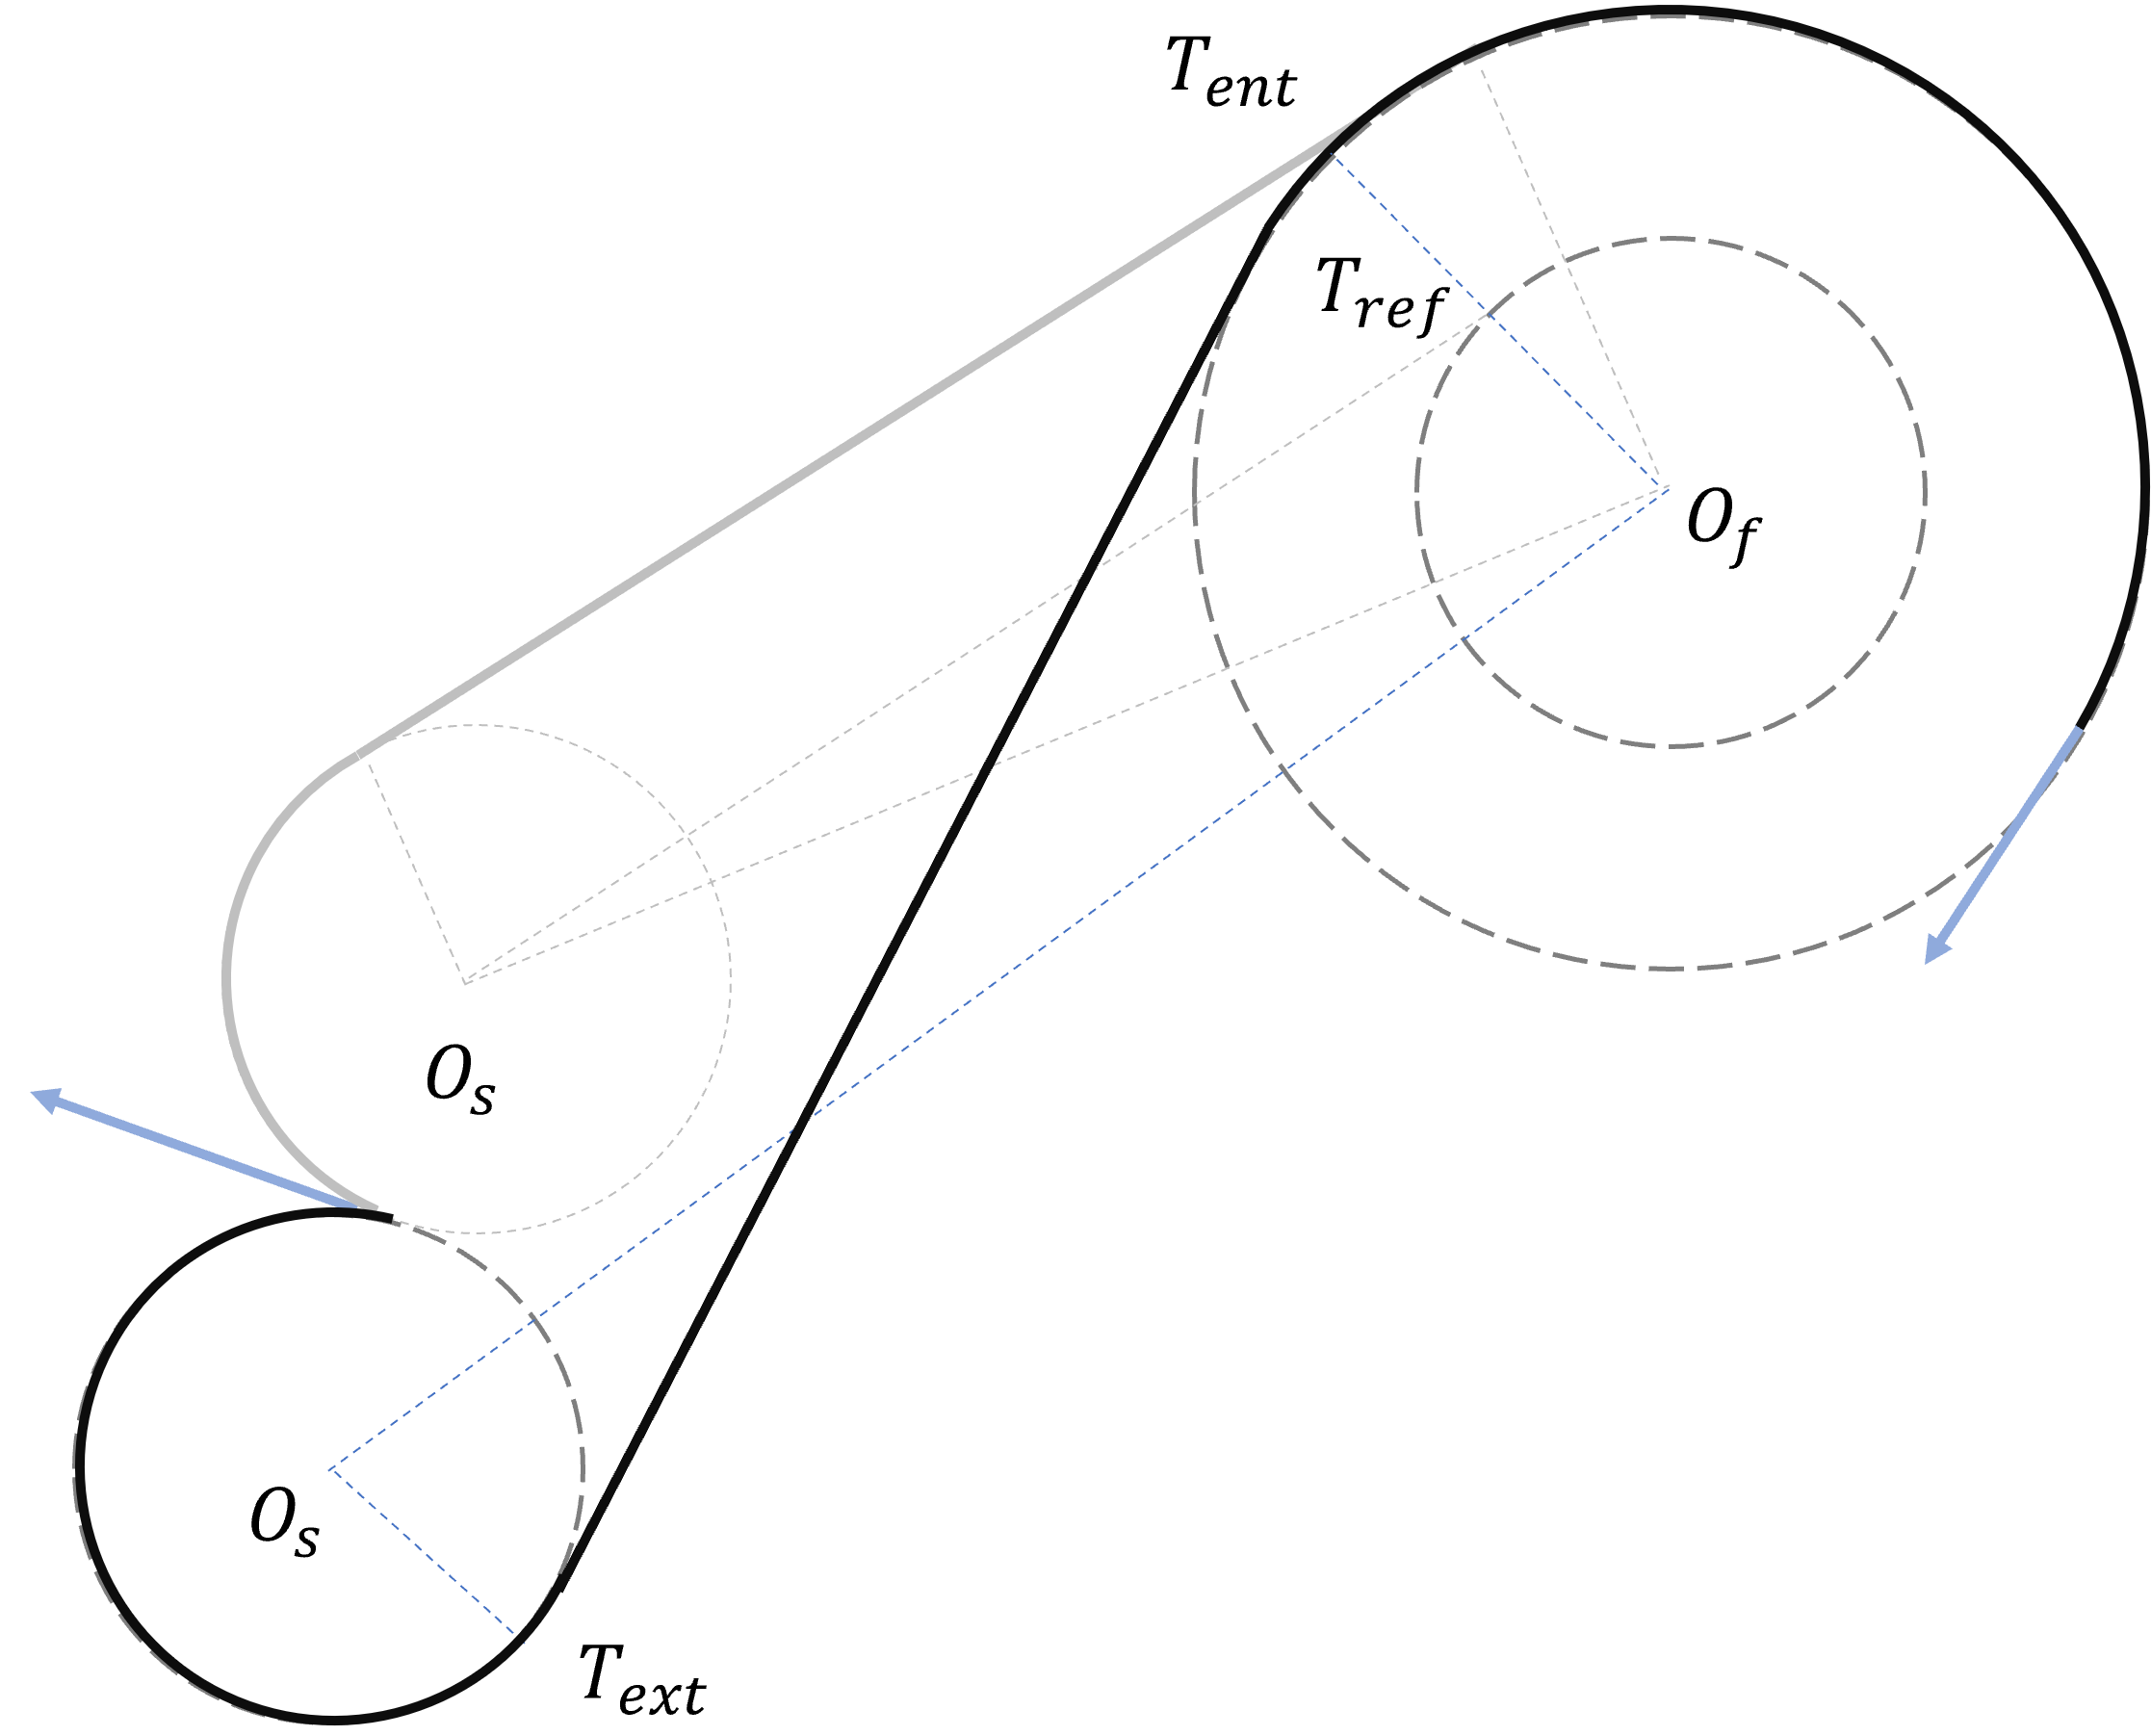
\includegraphics[width=0.7\linewidth]{fig/dubins/dubins_construction_lsr.png}
         \caption{Dubins construction following LSR pattern, the pattern for RSR is in grey color for comparison}
         \label{fig: dubins pattern consturction LSR}
     \end{subfigure}
        \caption{Different Dubins contruction pattern for the same start and finish condition}
        \label{fig:dubins pattern difference for same condition}
\end{figure}

\section{LQR controller design for TTWR}

The first control algorithm implemented in the traditional hierarchy TTWR controller is the Linear Quadratic Regulator (LQR). As defined in Section \ref{section: ttwr system analysis}, the system $(\mathcal{A}, \mathcal{B})$ is controllable by analysing its controllaiblity grammian or by applying Cayley-Hamilton theorem to its controllability matrix, which indicates that it is possible to manipulate the eigen values of the closes loop system $(\mathcal{A} - \mathcal{B}K)$ by choosing the state feed back control law $u = -K x$. Similarly, the LQR algorithm is a widely used algorithm to find an appropriate state-feedback controller. LQR controllers possess inherent robustness with guaranteed gain and phase margin \parencite{lehtomaki1981robustness}, and LQR plays a crucial role in addressing the LQG (linear–quadratic–Gaussian) challenge, which is the foundational problems in control theory.

For a controllable system, given either full-state measurements or full-state estimate, there exists more than one control laws, $u = - K x$, which stabilize the system states, and the eigenvalues of the closed-loop system, $(A - B K)$, can be designed and placed to left-half of the complex plane to achieve system stability. However, over stability by choosing large negative eigenvalues might require significant large control efforts, and may exceed the system input limitation, cause a wast of control energy, and reduce the system robustness for certain noise and disturbance. Therefore, the balance between stability of the closed loop system and the aggressiveness of the control input is the main purpose in optimal control, which is achieved by choosing the most suitable gain matrix K to stabilize the system without expending too much control effort. Three rules shall be taken into consideration when choosing the proper control gain, which incluldes \parencite{brunton2022data}:

\begin{itemize}
    \item prevent the controller from overreacting to high-frequency noise and disturbances
    \item the control actuation does not exceed limitation
    \item the control effort is not prohibitively expensive
\end{itemize}

For an infinite-horizon, continuous-time system described in Equation \ref{eqn: lti system states}, the cost function defined as:
\begin{equation}
    J=\int_0^{\infty}\left(x^T Q x+u^T R u+2 x^T N u\right) d t
    \label{eqn: lqr control cost function}
\end{equation}
where the matrices $Q$ and $R$ weight the cost of state deviation and actuation cost respectively, the matrix $Q$ is positive semi-definite, and $R$ is positive definite; these matrices are often diagonal, and the diagonal elements can be tuned to change the relative importance of the control objectives.

\begin{figure}
    \centering
    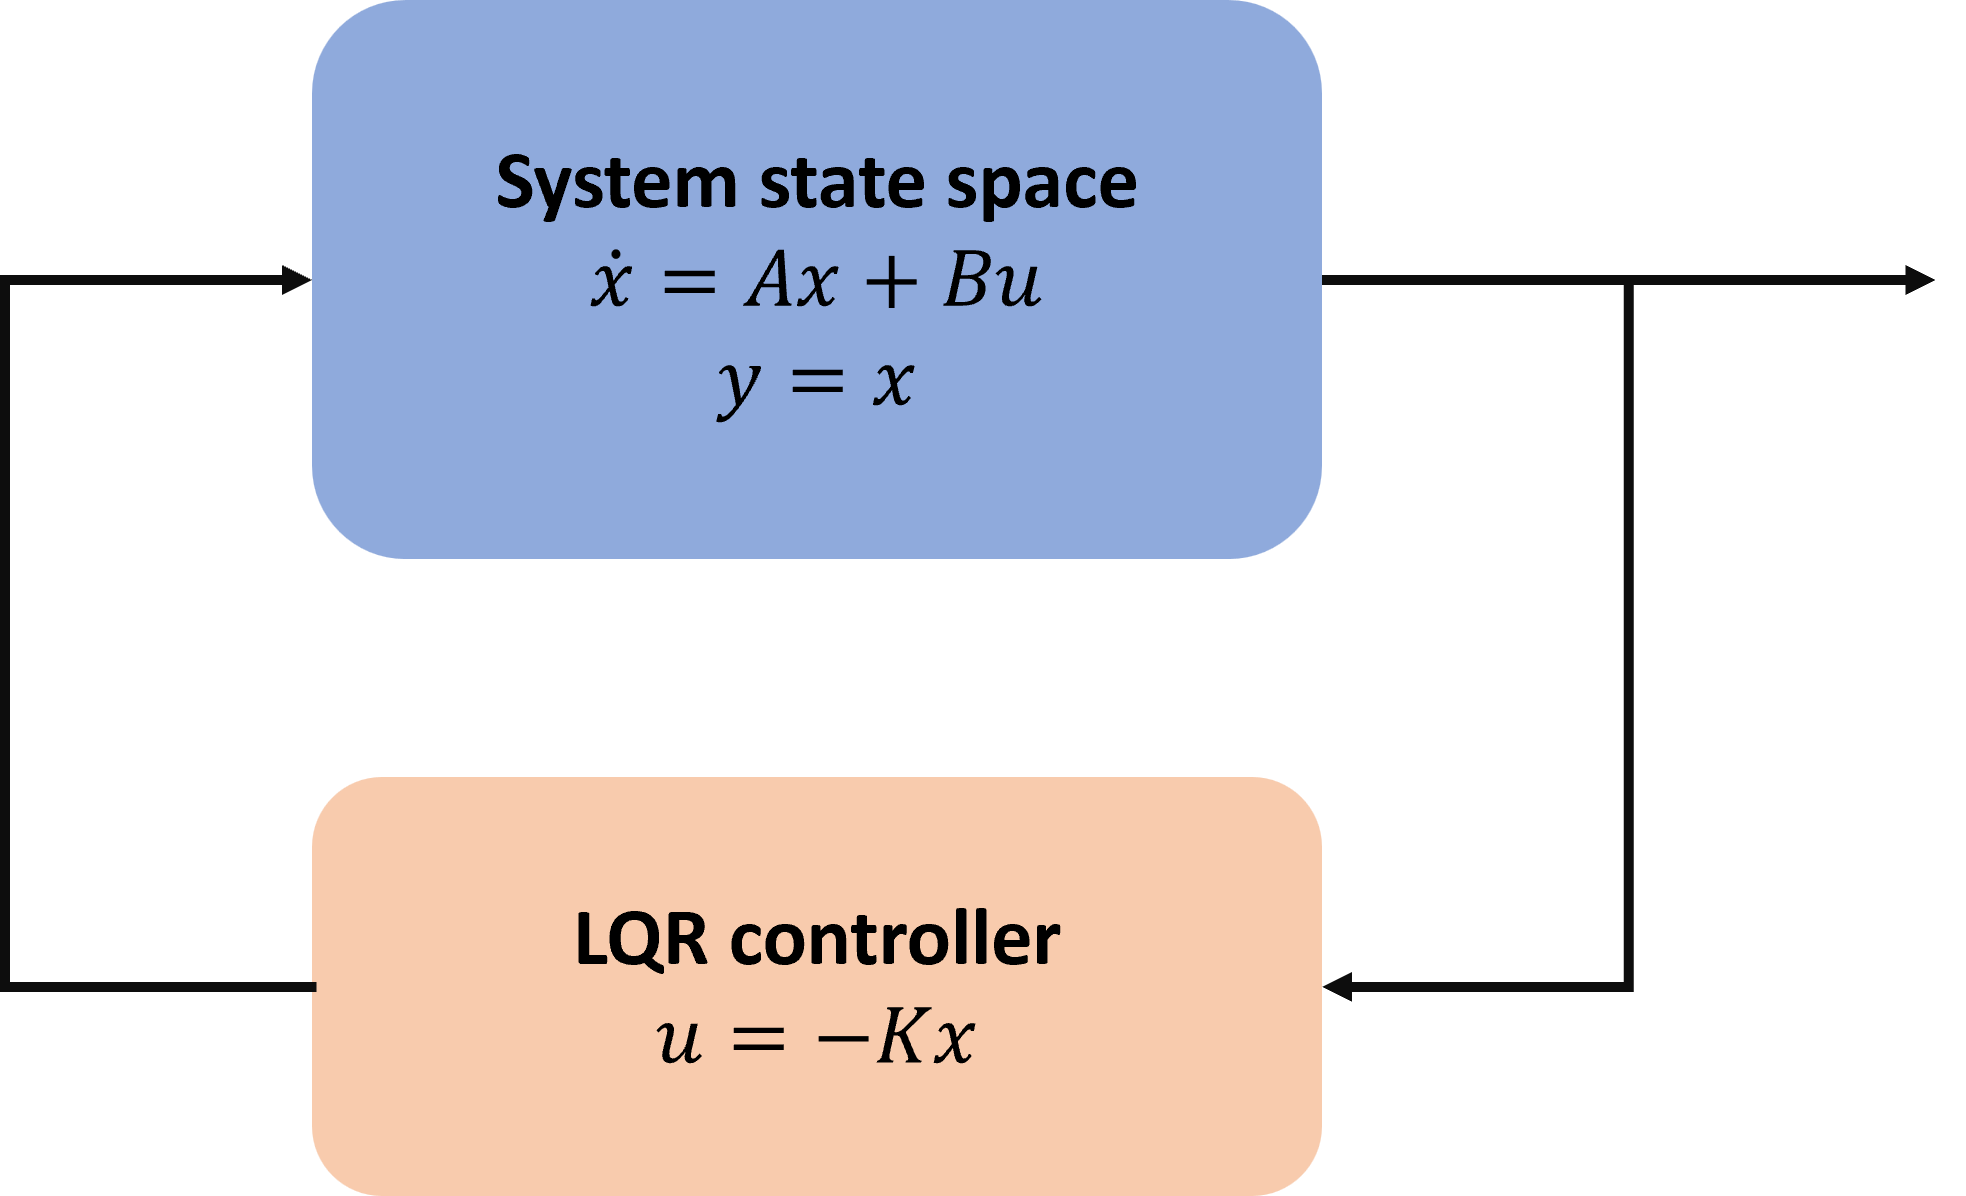
\includegraphics[width=0.5\linewidth]{fig/lqr_control_example.png}
    \caption{LQR controller schematic diagram}
    \label{fig: LQR controller schematic diagram}
\end{figure}

The weight matrix is useful to make choices to optimize the control law, for example, a larger value in a particular diagonal entry of $Q$ matrix means that deviations in the corresponding state will be penalized more heavily in the cost function. This will lead the controller to work harder to regulate the particular state. When the $Q$ matrix is set to be zero, the controller will not attempt to regulate the state at all, focusing solely on minimizing control effort. The matrix $R$ determines how much the control actions are penalized in the cost function. A larger value in a diagonal entry of R means that the corresponding control action will be penalized more. This discourages aggressive control actions and can be used to ensure smoother control signals. If R is too small, the controller might become overly aggressive, leading to large control signals that could saturate actuators or cause wear and tear.

As shown in Figure \ref{fig: LQR controller schematic diagram}, the LQR control law $u = - K x$ is designed to minimize the cost function $J=\lim _{t \rightarrow \infty} J(t)$. As its name suggests, LQR is a control strategy formulated for linear systems and employs the linear control law to minimize a cost function defined quadratically, aims to optimally regulate the system's state $\lim _{t \rightarrow \infty} \mathbf{x}(t)=0$. The analytical solution for the optimal controller gain $K$ can be computed following:
\begin{equation}
    K=R^{-1}\left(B^T P+N^T\right)
\end{equation}
and the variable $P$ is found by solving the continuous time algebraic Riccati equation:
\begin{equation}
    A^T P+P A-(P B+N) R^{-1}\left(B^T P+N^T\right)+Q=0
\end{equation}
which can be also written as:
\begin{equation}
    \mathcal{A}^T P+P \mathcal{A}-P B R^{-1} B^T P+\mathcal{Q}=0
\end{equation}
with
\begin{equation}
    \mathcal{A}=A-B R^{-1} N^T \quad \mathcal{Q}=Q-N R^{-1} N^T
\end{equation}

\begin{figure}
    \centering
    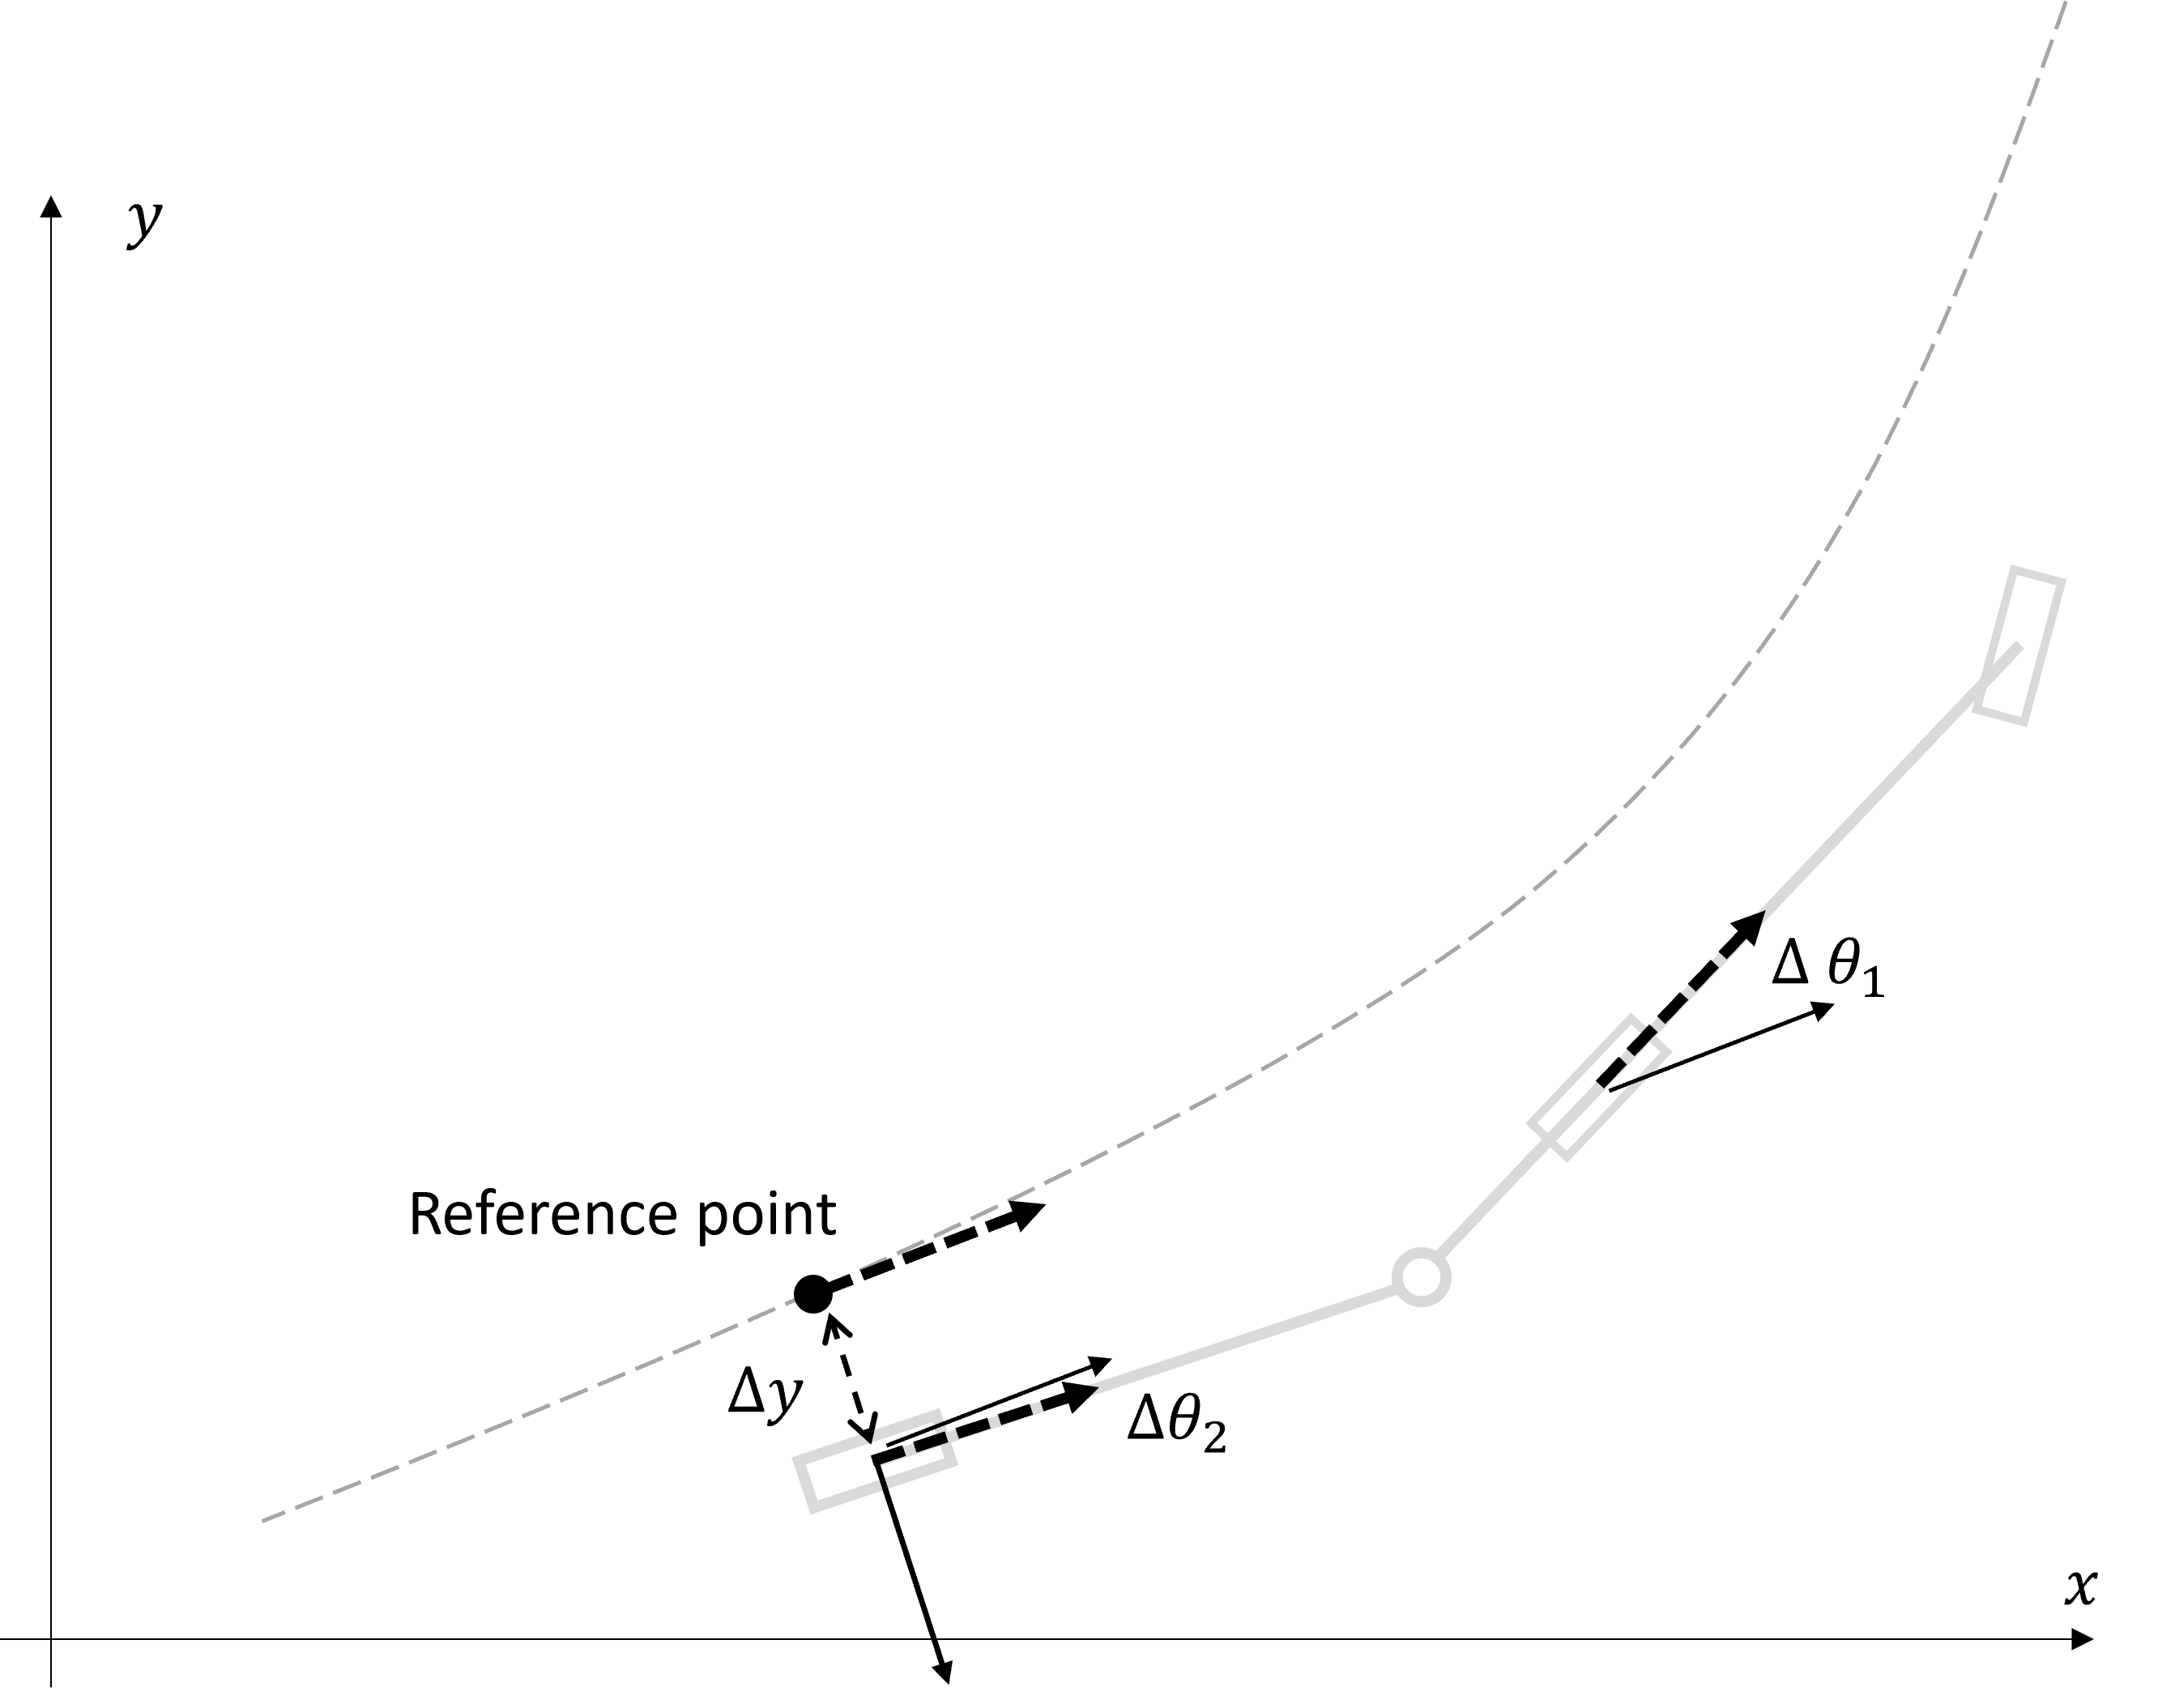
\includegraphics[width=0.7\linewidth]{fig/lateral distance error.png}
    \caption{LQR controller reference states error}
    \label{fig: LQR controller reference states error}
\end{figure}

For the TTWR control topic, the state equation can be formulated as:
\begin{equation} 
\begin{bmatrix}
    \Delta \dot{\theta_1} \\ \Delta \dot{\theta_2} \\ \Delta \dot{y}
\end{bmatrix} = \begin{bmatrix}
0 & 0 & 0 \\
\frac{v}{L_3} & -\frac{v}{L_3} & 0 \\
0 & V & 0
\end{bmatrix}   \begin{bmatrix}
    \Delta \theta_1 \\ \Delta \theta_2 \\ \Delta y
\end{bmatrix} + \begin{bmatrix}
    \frac{v}{L_1} \\ -\frac{L_2}{L_1  L_3} v \\ 0
\end{bmatrix} \delta \label{eq: lqr state space}\end{equation}
as shown in Figure \ref{fig: LQR controller reference states error}, the reference states error consist of $\Delta \theta_1$, $\Delta \theta_2$, and $\Delta y$, which represents the heading error between TTWR's truck heading angle and the reference point heading angle, the heading error between trailer heading angle and reference point heading angle, and the lateral distance in trailer coordinate between trailer position and refernece point.

To compute the optimal gain of the TTWR controller, MATLAB provides built-in functions which can solve Riccati equation efficiently by providing the system state space model, weight matrix $Q$ and $R$, the code is as following:

\begin{lstlisting}[
frame=single,
numbers=left,
style=Matlab-Pyglike]
% TTWR parameters
L1 = 3; % truck wheelbase length [m]
L2 = 2; % hitch length [m] 
L3 = 1.5; % trailer wheelbase length [m] 
vx = -2; % truck longitudinal velocity [m/s] 

% Linearized State Space
A = [0       0         0;
     vx./L3  -vx./L3   0;
     0       vx        0];

B = [vx./L1;
     -L2*vx ./ (L1*L3);
     0];

C = eye(3);
D = zeros(3, 1);

% state states x = [\theta1, \theta2, \y_err]
sys = ss(A, B, C, D);

% State weight matrix
% \theta1 and \theta2 error ref for 2 degrees, and  
% lateral error reference value is 0.8
Q = [1/(deg2rad(2).^2)       0                       0;
     0                   1/(deg2rad(2).^2)           0;
     0                        0                1/(0.8.^2)];
% Input weight matrix for steering angle
R = 1 / (deg2rad(steer_max).^2);

% Output K is the LQR gain
[K,S,P] = lqr(sys, Q, R)
\end{lstlisting}

\begin{figure}
    \centering
    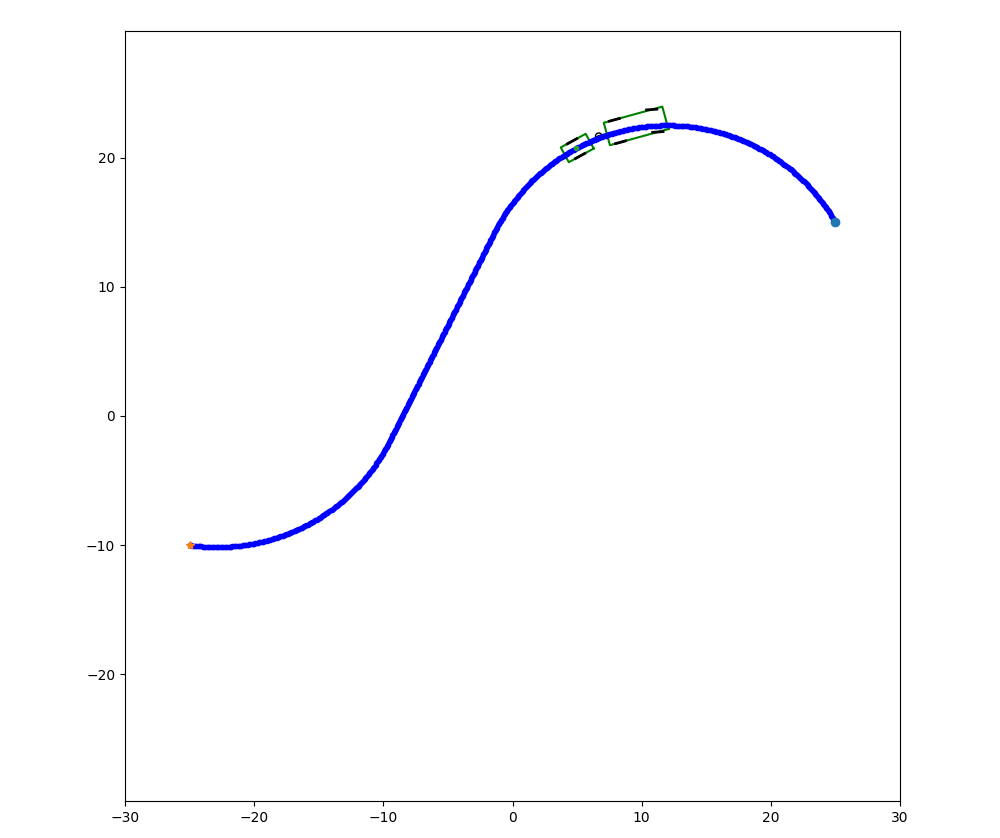
\includegraphics[width=0.8\linewidth]{fig/lqr/lqr_path_following.png}
    \caption{The simulation of using Dubins and LQR for TTWR reverse driving control}
    \label{fig: simulation of using Dubins and LQR for TTWR reverse driving control}
\end{figure}

\begin{figure}
    \centering
    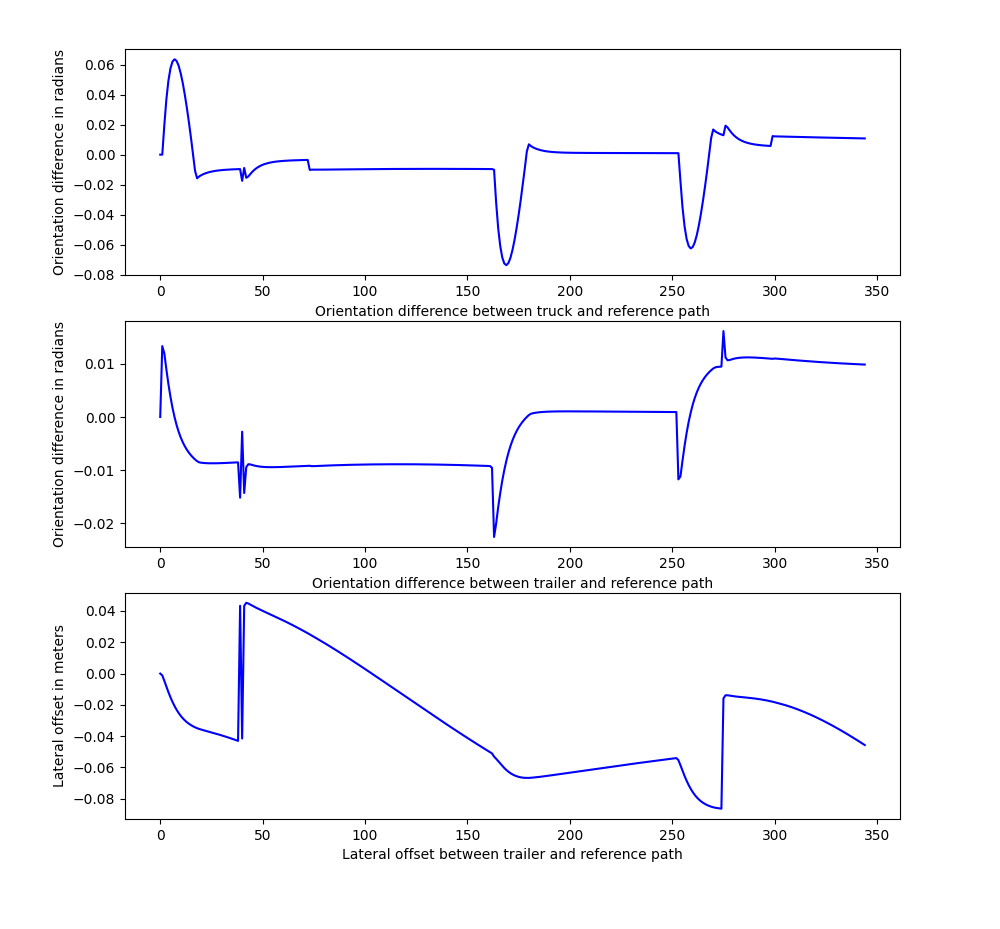
\includegraphics[width=0.7\linewidth]{fig/lqr/lqr states.png}
    \caption{The system states of the LQR controller}
    \label{fig: system states of the LQR controller}
\end{figure}

The results of the LQR TTWR reverse path following control is shown in Figures \ref{fig: simulation of using Dubins and LQR for TTWR reverse driving control}, which depict the reference trajectory and the TTWR vehicle states respectively. The blue line is the Dubins trajectory started with initial states $(25, 25, -\frac{\pi}{3})$ and final states $(-25. -10, 0)$ which is lateral offset between trajectory and truck or trailer, and the heading angle difference between trajectory and trailer. The Figure \ref{fig: system states of the LQR controller} shows the TTWR states along the path following task, and the lateral offset of truck and traler are both within 0.1 meters, and the heading angle difference is also within 0.1 rad. The LQR controller effectively ensures that the articulated vehicle system follows closely to the desired trajectory. This is evident from the gentle turning motions observed whenever the blue line alters its direction. Moreover, the consistent spacing between each sample signifies a gradual and smooth turning process, highlighting the controller's efficiency in maintaining steady and controlled maneuvers.

\clearpage

\section{MPC controller design for TTWR}
\label{MPC controller design for TTWR}
Model Predictive Control (MPC) operates by executing finite-horizon optimization for a system model at each discrete time step. The primary idea behind MPC is to use a model of the system to predict its future behavior over a finite horizon. Based on this prediction, the control inputs are determined by minimizing a cost function, which typically represents a combination of tracking errors and control efforts.
\begin{equation}
J = \sum_{k=0}^{N-1} \left( x(k)^T Q x(k) + u(k)^T R u(k) \right) + x(N)^T P x(N)
\end{equation}
where $J$ is the cost to be minimized, $N$ is the prediction horizon, $X_k$ is the system states at time $t_k$, $U_k$ is the input states at time $t_k$, and $Q$ and $R$ is the weight matrix for system states and control input respectively, and these two matrices are designed to be positive definite, and the $P$ is the terminal cost wight matrix.

At every instance $t_k$, the system is sampled, and a control strategy is derived for the control horizon $[t_k, t_k + N_C]$ to minimize the deviation from the desired trajectory over the prediction horizon $[t_k, t_k + N_P]$. Beyond $N_C$ control moves, the control input remains constant for the rest of the prediction horizon. The system's progression is forecasted using an intrinsic mathematical model, and a numerical optimization technique minimizes the control cost. Only the initial control input from the determined sequence is implemented at each time step $t_k$. This procedure is repeated in every cycle, with both the control and prediction horizons advancing forward. The principle of the MPC algorithm is shown in Figure \ref{fig: Function principle of a model-based predictive}.

\begin{figure}
    \centering
    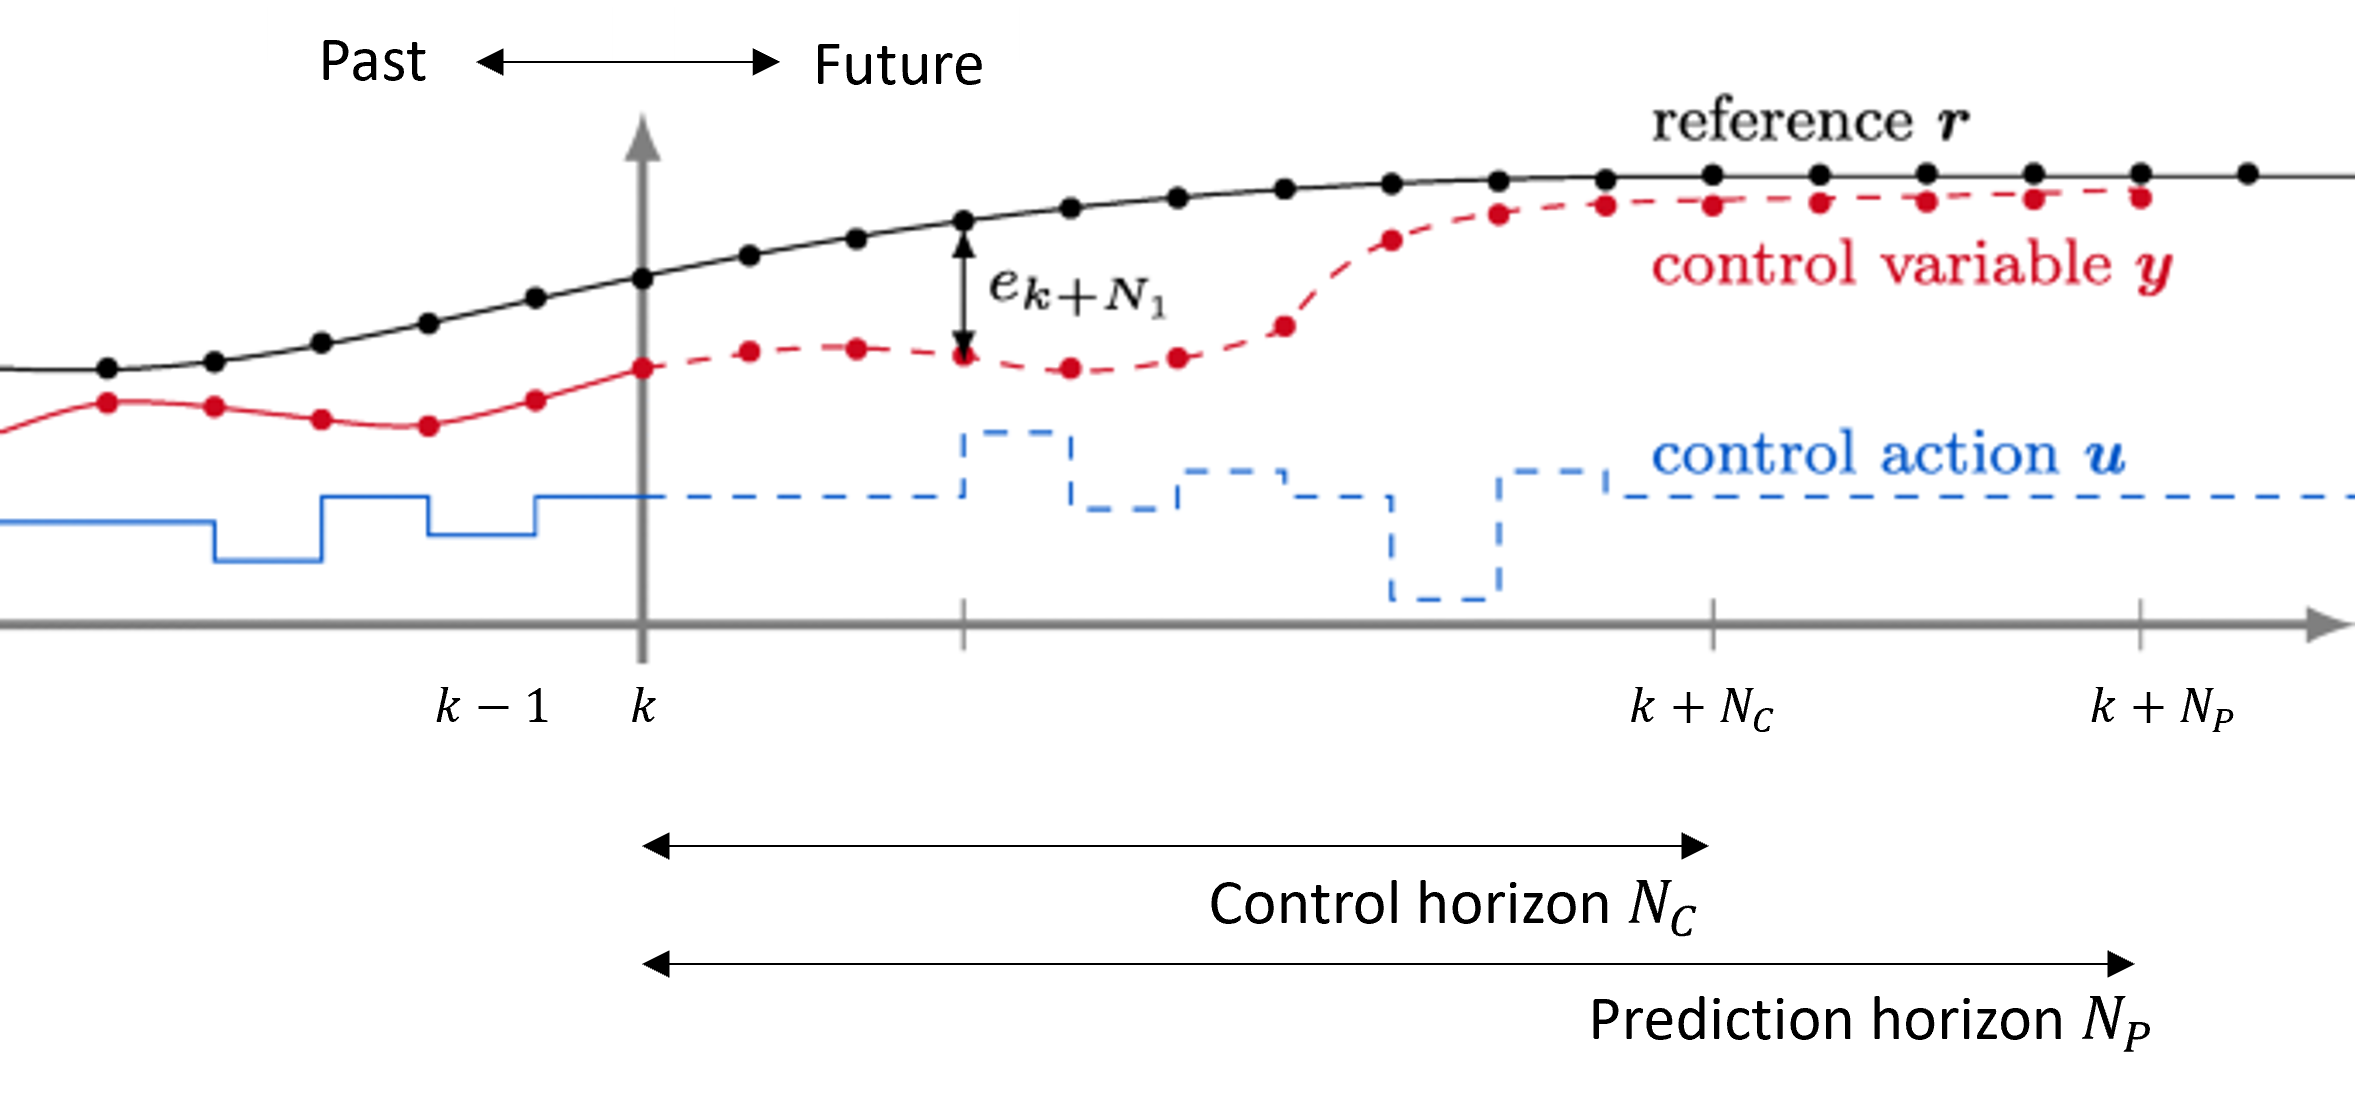
\includegraphics[width=0.7\linewidth]{fig/mpc/mpc_examples.png}
    \caption{Function principle of a model-based predictive \parencite{schwenzer2021review}}
    \label{fig: Function principle of a model-based predictive}
\end{figure}

To describe the TTWR system state space trasfer function, a new state variable $v_1$ is added for referencing, and then the state vector becomes $X = [x_1, y_1, \theta_1, x_2, y_2, theta_2, phi, v]$, and the input states change from $U = [v, \delta]$ to $U = [a, \delta]$ where $a$ is the acceleration of the truck vehicle. The new state representation is as following:

\begin{equation}
    \begin{aligned} 
        \dot{x}_1 &= f_1(X ,U)= v \cos{\theta_1} \\ 
        \dot{y}_1 &= f_2(X ,U) = v \sin{\theta_1} \\ 
        \dot{\theta}_1 &= f_3(X ,U) = \frac{v}{L_1}\tan{\delta} \\ 
        \dot{x}_2 &= f_4(X ,U) = v \cos{\phi} (1 - \frac{L_2}{L_1}\tan{\phi}\tan{\delta})\cos{\theta_2} \\ 
        \dot{y}_2 &= f_5(X ,U) = v \cos{\phi} (1 - \frac{L_2}{L_1}\tan{\phi}\tan{\delta})\sin{\theta_2} \\ 
        \dot{\theta}_2 &= f_6(X ,U) = -v (\frac{\sin{\phi}}{L_3} + \frac{L_2}{L_1 L_3}\cos{\phi}\tan{\delta} ) \\ 
        \dot{\phi} &= f_7(X ,U) = -\frac{v}{L_3}\sin{\phi} - \frac{v}{L_1} ( 1 + \frac{L_2 \cos{\phi}}{L_3}) \tan{\delta} \\ 
        \dot{v_1}_1 &= f_8(X ,U) = a \\ 
    \end{aligned} 
\end{equation}

To get the Jacobian matrix $A'$ of the TTWR system, compute the partial derivatives of state transfer function $f_1$ to $f_8$ with respect to each elements in the state vector $X$:

\begin{equation}
   A' = 
    \begin{bmatrix}
    \frac{\partial f_1}{\partial x_1} & \frac{\partial f_1}{\partial y_1} & \frac{\partial f_1}{\partial \theta_1} & \frac{\partial f_1}{\partial x_2} & \frac{\partial f_1}{\partial y_2} & \frac{\partial f_1}{\partial \theta_2} & \frac{\partial f_1}{\partial \phi} & \frac{\partial f_1}{\partial v_1} \\
    \frac{\partial f_2}{\partial x_1} & \frac{\partial f_2}{\partial y_1} & \frac{\partial f_2}{\partial \theta_1} & \frac{\partial f_2}{\partial x_2} & \frac{\partial f_2}{\partial y_2} & \frac{\partial f_2}{\partial \theta_2} & \frac{\partial f_2}{\partial \phi} & \frac{\partial f_2}{\partial v_1} \\
    \frac{\partial f_3}{\partial x_1} & \frac{\partial f_3}{\partial y_1} & \frac{\partial f_3}{\partial \theta_1} & \frac{\partial f_3}{\partial x_2} & \frac{\partial f_3}{\partial y_2} & \frac{\partial f_3}{\partial \theta_2} & \frac{\partial f_3}{\partial \phi} & \frac{\partial f_3}{\partial v_1} \\
    \frac{\partial f_4}{\partial x_1} & \frac{\partial f_4}{\partial y_1} & \frac{\partial f_4}{\partial \theta_1} & \frac{\partial f_4}{\partial x_2} & \frac{\partial f_4}{\partial y_2} & \frac{\partial f_4}{\partial \theta_2} & \frac{\partial f_4}{\partial \phi} & \frac{\partial f_4}{\partial v_1} \\
    \frac{\partial f_5}{\partial x_1} & \frac{\partial f_5}{\partial y_1} & \frac{\partial f_5}{\partial \theta_1} & \frac{\partial f_5}{\partial x_2} & \frac{\partial f_5}{\partial y_2} & \frac{\partial f_5}{\partial \theta_2} & \frac{\partial f_5}{\partial \phi} & \frac{\partial f_5}{\partial v_1} \\
    \frac{\partial f_6}{\partial x_1} & \frac{\partial f_6}{\partial y_1} & \frac{\partial f_6}{\partial \theta_1} & \frac{\partial f_6}{\partial x_2} & \frac{\partial f_6}{\partial y_2} & \frac{\partial f_6}{\partial \theta_2} & \frac{\partial f_6}{\partial \phi} & \frac{\partial f_6}{\partial v_1} \\
    \frac{\partial f_7}{\partial x_1} & \frac{\partial f_7}{\partial y_1} & \frac{\partial f_7}{\partial \theta_1} & \frac{\partial f_7}{\partial x_2} & \frac{\partial f_7}{\partial y_2} & \frac{\partial f_7}{\partial \theta_2} & \frac{\partial f_7}{\partial \phi} & \frac{\partial f_7}{\partial v_1} \\
    \frac{\partial f_8}{\partial x_1} & \frac{\partial f_8}{\partial y_1} & \frac{\partial f_8}{\partial \theta_1} & \frac{\partial f_8}{\partial x_2} & \frac{\partial f_8}{\partial y_2} & \frac{\partial f_8}{\partial \theta_2} & \frac{\partial f_8}{\partial \phi} & \frac{\partial f_8}{\partial v_1} \\
    \end{bmatrix}
\end{equation}

The result of the partial derivatives is computed below, where the partial derivatives not listed are equal to zero:

\begin{equation}
\begin{aligned} 
    \frac{\partial f_1}{\partial \theta_1} &= -v_1 \sin{\theta_1} \\
    \frac{\partial f_1}{\partial v_1} &= cos\theta_1  \\
    \frac{\partial f_2}{\partial \theta_1} &= v_1 sin\theta_1  \\
    \frac{\partial f_2}{\partial v_1} &= sin\theta_1  \\
    \frac{\partial f_3}{\partial v_1} &= \frac{\tan{\delta}}{L_1}  \\
    \frac{\partial f_4}{\partial \theta_2} &= v\cos\phi(1-\frac{L_2}{L_1}\tan\delta\tan\phi)(-\sin{\theta_2})  \\
    \frac{\partial f_4}{\partial \phi} &= v (-\sin{\phi}) (1-\frac{L_2}{L_1}\tan{\delta}\tan{phi})\cos{\theta_2}\\
            &+v\cos{\phi}(-\frac{L_2}{L_1}*\sec{\phi} \tan{\delta})\cos{theta_2}  \\
    \frac{\partial f_4}{\partial v_1} &= \cos{\phi}(1 - \frac{L_2}{L_1}\tan{phi}\tan{\delta})\cos{\theta_2}  \\
    \frac{\partial f_5}{\partial \theta_2} &= v\cos\phi(1-\frac{L_2}{L_1}\tan\delta\tan\phi)\cos{\theta_2}  \\
    \frac{\partial f_5}{\partial \phi} &= v (-\sin{\phi}) (1-\frac{L_2}{L_1}\tan{\delta}\tan{phi})\sin{\theta_2}\\
            &+v\cos{\phi}(-\frac{L_2}{L_1}*\sec{\phi} \tan{\delta})\sin{theta_2}  \\
    \frac{\partial f_5}{\partial v_1} &= \cos{\phi}(1 - \frac{L_2}{L_1}\tan{phi}\tan{\delta})\sin{\theta_2}  \\
    \frac{\partial f_6}{\partial \phi} &= -v_1 (\frac{\cos{\phi})}{L_3} -\frac{L_2}{L_1 L_3} \sin{phi} \tan{delta})  \\
    \frac{\partial f_6}{\partial v_1} &= -(\frac{\sin{\phi}}{L_3} + \frac{L_2}{L_1 L_3}\cos{\phi}\tan{\delta} )  \\
    \frac{\partial f_7}{\partial \phi} &= -\frac{v}{L_3}\cos{\phi} - \frac{v}{L_1} ( 1 - \frac{L_2 \sin{\phi}}{L_3}) \tan{\delta}  \\
    \frac{\partial f_7}{\partial v_1} &= -\frac{1}{L_3}\sin{\phi} - \frac{1}{L_1} ( 1 + \frac{L_2 \cos{\phi}}{L_3}) \tan{\delta}  
\end{aligned}   
\end{equation}

And similarly, the matrix $B'$ can be wrriten as:

\begin{equation}
    B' = 
    \begin{bmatrix}
    \frac{\partial f_1}{\partial \delta} & \frac{\partial f_1}{\partial a} \\
    \frac{\partial f_2}{\partial \delta} & \frac{\partial f_2}{\partial a} \\
    \frac{\partial f_3}{\partial \delta} & \frac{\partial f_3}{\partial a} \\
    \frac{\partial f_4}{\partial \delta} & \frac{\partial f_4}{\partial a} \\
    \frac{\partial f_5}{\partial \delta} & \frac{\partial f_5}{\partial a} \\
    \frac{\partial f_6}{\partial \delta} & \frac{\partial f_6}{\partial a} \\
    \frac{\partial f_7}{\partial \delta} & \frac{\partial f_7}{\partial a} \\
    \frac{\partial f_8}{\partial \delta} & \frac{\partial f_8}{\partial a} \\
    \end{bmatrix}
\end{equation}
where the partial derivatives of equations $f_1$ to $f_8$ with respect to input variables can be written as the following (similarly, the rest of the partial derivatives is 0):

\begin{equation}
    \begin{aligned} 
        \frac{\partial f_8}{\partial a} &= 1\\
        \frac{\partial f_3}{\partial \delta} &= \frac{v_1}{L_1} \sec{\delta} \\
        \frac{\partial f_4}{\partial \delta} &= - v_1 \cos{\phi} \frac{L_2}{L_1} \tan{phi} \sec{\delta} \cos{\delta} \\
        \frac{\partial f_5}{\partial \delta} &= - v_1 \cos{\phi} \frac{L_2}{L_1} \tan{phi} \sec{\delta} \sin{\delta} \\
        \frac{\partial f_6}{\partial \delta} &= - v_1 \frac{L_2}{L_1 L_3} \cos{\phi} \sec{\delta} \\
        \frac{\partial f_7}{\partial \delta} &= - \frac{v_1}{L_1} (1 + \frac{L_2}{L_3} \cos{\phi}) \sec{\delta} \\
    \end{aligned} 
\end{equation}

Then, using the methods of Forward Euler Discretization with sampling time $dt$, the state transfer equation can be written as:

\begin{equation}
X_{k+1}=X_k+f\left(X_k, U_k\right) dt
\end{equation}

Using first degree Tayer expantion around $\bar{X}$ and $\bar{U}$
\begin{equation}
\begin{aligned}
X_{k+1}&=X_k+\left(f(\bar{X}, \bar{U})+A^{\prime} z_k+B^{\prime} U_k-A^{\prime} \bar{X}-B^{\prime} \bar{U}\right) d t \\
X_{k+1}&=\left(I+d t A^{\prime}\right) X_k+\left(d t B^{\prime}\right) U_k+\left(f(\bar{X}, \bar{U})-A^{\prime} \bar{X}-B^{\prime} \bar{U}\right) d t
\end{aligned}
\label{eqn: tayler expansion of linearization}
\end{equation}

The equation \ref{eqn: tayler expansion of linearization} can be transferd to the form following state space control schema: 
\begin{equation}
x_{k+1}=A x_k+B U_k+C
\end{equation}
where the $A$, $B$, and $C$ can be replaced using the derived Jacobian matrix:
\begin{equation}
\begin{aligned}
& A=\left(I+d t A^{\prime}\right) \\
& B=d t B^{\prime} \\
& C=\left(f(\bar{z}, \bar{u})-A^{\prime} \bar{z}-B^{\prime} \bar{u}\right) d t
\end{aligned}
\end{equation}

\section{Proximal Policy Optimization based end-to-end control algorithm}
\label{section: PPO based end to end control algorithm}

* this section is from the first published journal paper \cite{Yan_Zohdy_Shaout_Mahmoud_2023}

The Proximal Policy Optimization (PPO) method is an improved policy gradient (PG) reinforcement learning technique introduced in 2017 by OpenAI \parencite{schulman2017proximal}. It is characterized as an unconstrained optimization problem comprising two components: cumulative discounted return and Kullback–Leibler (KL) divergence \parencite{xu2023improving}. Compared with other DRL algorithms, PPO demonstrates improved data efficiency, reduced computational demands, and a reduced likelihood of policy divergence or catastrophic memory loss.

The foundation of the PG method lies in the calculation of the policy gradient estimator and its application within a stochastic gradient ascent framework. A frequently used gradient estimator can be written as:
\begin{equation}
\hat{g}=\hat{\mathbb{E}}_t\left[\nabla_\theta \log \pi_\theta\left(a_t \mid s_t\right) \hat{A}_t\right]
\label{eq: function gradient estimator}
\end{equation}
where $\pi_\theta$ is a stochastic policy and $\hat{A}_t$ is an estimator at timestep $t$, and $\hat{\mathbb{E}}_t[\ldots]$ is empirical average over a finite batch of samples. The estimator $\hat{g}$ can be computed by differentiating the objective
\begin{equation}
L^{P G}(\theta)=\hat{\mathbb{E}}_t\left[\log \pi_\theta\left(a_t \mid s_t\right) \hat{A}_t\right]
\label{eq: PG objective}
\end{equation}
where $\hat{A}_t$ is the estimator of the advantage function at timestep $t$, and $\pi_\theta$ is a stochastic policy.

A challenge with the PG method is its sensitivity to step size, complicating the task of selecting an appropriate step size. To address this unconstrained optimization challenge, drawing inspiration from the Trust Region Policy Optimization (TRPO) method \parencite{schulman2015trust}, the objective function is maximized using the ratio of prior strategies $\pi_{\theta_{\text{old}}}$ to new strategies $\pi_{\theta}$, while penalizing the magnitude of the policy update with coefficient $\beta$:
\begin{equation}
\underset{\theta}{\operatorname{maximize}} 
 \hat{\mathbb{E}}_t\left[\frac{\pi_\theta\left(a_t \mid s_t\right)}{\pi_{\theta_{\text {old }}}\left(a_t \mid s_t\right)} \hat{A}_t - \beta \mathrm{KL}\left[\pi_{\theta_{\text {old }}}\left(\cdot \mid s_t\right), \pi_\theta\left(\cdot \mid s_t\right)\right]\right]
\label{eq: pg optimization problem}
\end{equation}
where the probability ratio of old and new strategies is denoted as $r_t(\theta)$ in following equations. 

To penalize the excessively large policy update caused when maximizing the objective $L^{CPI}$, the PPO algorithm penalizes changes to the policy that move $r_t(\theta)$ away from 1, and get the main objective function:
\begin{equation}
L^{CLIP}(\theta)=\hat{\mathbb{E}}_t\left[\min \left(r_t(\theta) \hat{A}_t, \operatorname{clip}\left(r_t(\theta), 1-\epsilon, 1+\epsilon\right) \hat{A}_t\right)\right]
\label{eq: PPO objective function}
\end{equation}
where the first term $L^{CPI}$ is derived from the TRPO method, and the second term, $\operatorname{clip}\left(r_t(\theta), 1-\epsilon, 1+\epsilon\right) \hat{A}_l$, represents the clip function which constrains the values of the old and new policy parameters $r_t(\theta)$ within the range $[1-\epsilon, 1+\epsilon]$. The final step involves the application of the min function to select the lesser value between the clipped and unclipped objectives.

\begin{figure}[h]
    \centering
    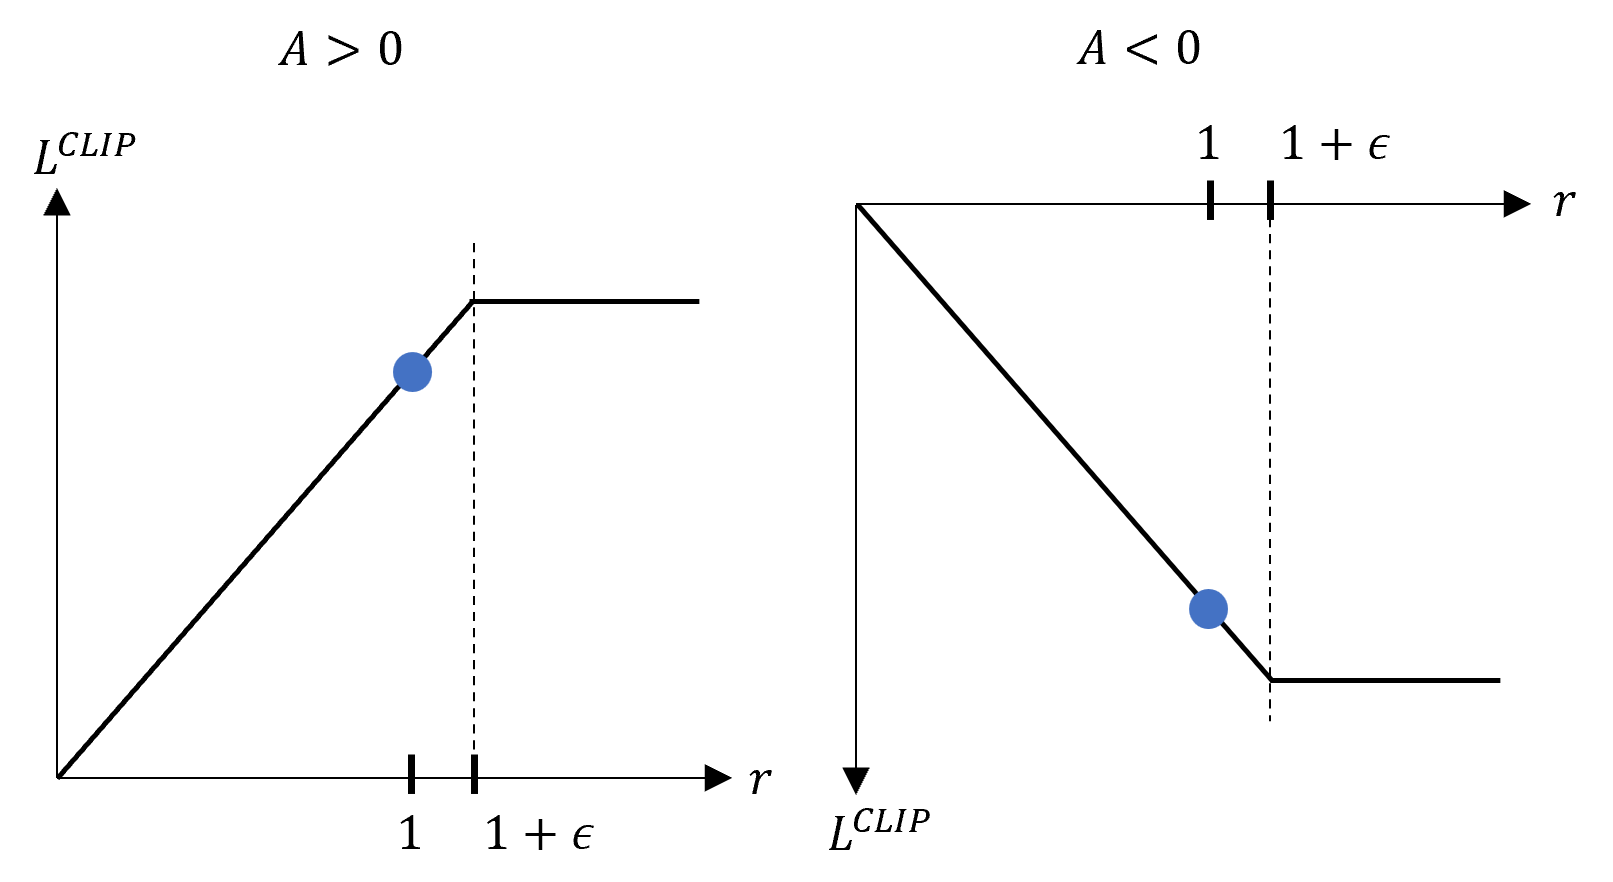
\includegraphics[width=0.6\linewidth]{fig/clip_function.png}
    \caption{Illustration of the clip function, where the probability ratio $r$ is clipped at $1-\epsilon$ or $1+\epsilon$ depending on the polarity of the advantage}
    \label{fig: clip function}
\end{figure}

The core philosophy of the PPO algorithm is to mitigate the challenges caused by large policy updates in the PG algorithm, which can it difficult for step sizes determination and low data efficiency. By adopting a clipping mechanism to avoid imposing hard constraint completely, the PPO is proven to be very effective in dealing with a wide range of challenging tasks, while being simple to implement and tune.

The architecture for the TTWR autonomous parking mechanism is depicted in Figure \ref{fig: TTWR training process}. This system is bifurcated into two primary components: a profound reinforcement learning module and a simulation framework. Specifically, the profound reinforcement learning module utilizes an LSTM-PPO technique to train the agent for mastering autonomous parking and evading obstacles, all while engaging with the entities within the parking milieu. The simulation framework encompasses the kinematic model of TTWR, static vehicular obstructions, parking spaces, and sonar-driven distance sensing, all realized in Matlab to engage with the training agent.

\begin{figure}[h]
    \centering
    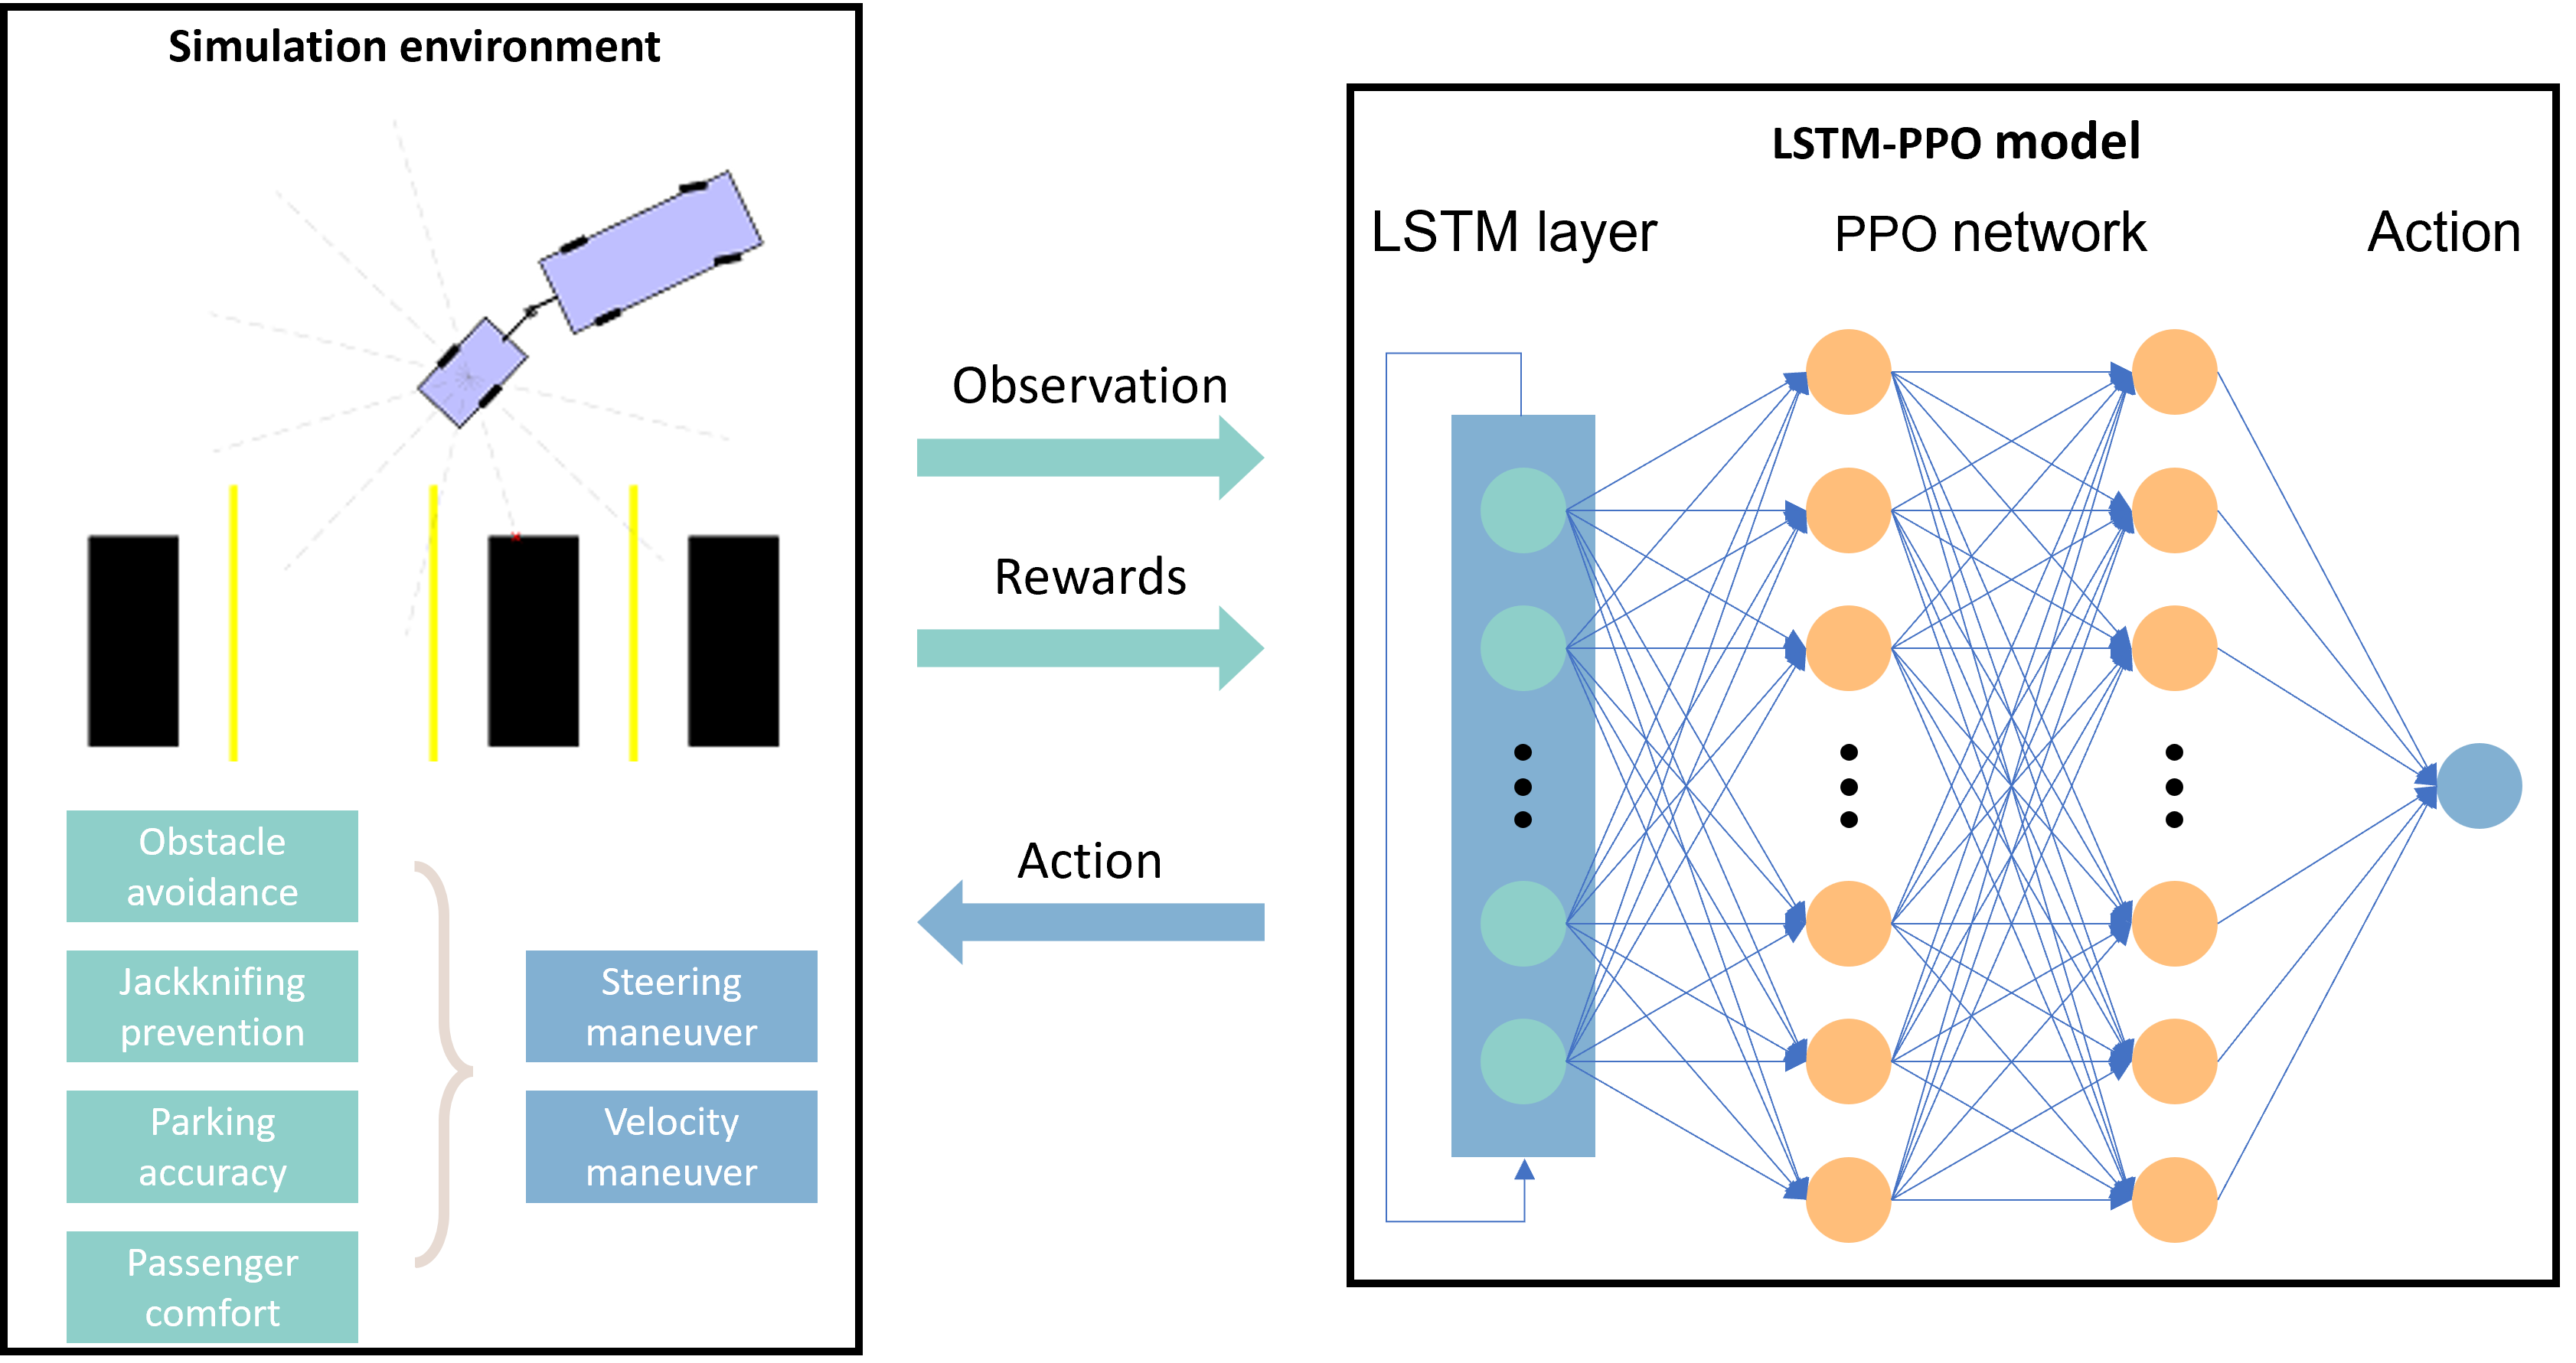
\includegraphics[width=0.9\linewidth]{fig/ppo/system_architecture.png}
    \caption{TTWR autonomous parking system layout}
    \label{fig: TTWR training process}
\end{figure}

The TTWR mechanism evaluates the parking target coordinates, TTWR system configurations, and the perceived obstacle data to execute the autonomous parking operation. To address the dimensionality challenges stemming from intricate observation data, the technique discretizes the obstacle perception data around the agent, sampling points within a predefined threshold. This allows for a more streamlined observation vector, represented as:

\begin{equation}
S_t = \left[\begin{array}{ccc}
S_\text{TTWR}, S_\text{sonar}, S_\text{goal}
\end{array}\right]^T
\label{eq: observation}
\end{equation}

Here, $S_\text{TTWR} = \left[\begin{array}{ccc} x_1, y_1, \theta_1, x_2, y_2, \theta_2, \phi\end{array}\right]^T$ represents the TTWR state configurations as defined by the kinematic model. The parking objective, $S_\text{goal} = \left[\begin{array}{ccc} x_\text{goal}, y_\text{goal}, \theta_\text{goal}\end{array}\right]^T$, signifies the desired parking location for the TTWR, determined by user input.

Furthermore, $S_\text{sonar}$ is the data from sonar instruments affixed to the trailer. Instead of a full $360^{\circ}$ environmental scan, the sonar provides distance measurements within its field of view. These readings can be transformed from polar to Cartesian coordinates to depict obstructions around the trailer. Specifically, the sonar readings, $S_\text{sonar}$, can be articulated as:

\begin{equation}
S_\text{sonar}=\left[\begin{array}{cccc}
dist_{1} & dist_{2} & \cdots & dist_{n}
\end{array}\right]
\label{eq: sonar observation}
\end{equation}

To enhance the driving experience and ensure fluid vehicle control, this study introduces an action module that represents the primary vehicle's steering input for lateral management. The steering controller prompts the agent to select the optimal action value from a continuous action domain, produced by the LSTM-PPO algorithm, and is defined within the range of $[-\delta_{max}, \delta_{max}]$, where $\delta_{max}$ is the utmost steering angle based on the primary vehicle's specifications.

The reward function acts as the feedback conduit for the controller, associating the current state and action of the TTWR to a scalar metric that evaluates potential maneuvers. Specifically, the reward function is crafted to guide the controller in learning how to adeptly park the trailer, emphasizing collision prevention and ensuring a seamless user experience.

\begin{itemize}
  \item Distance metric $R_{\text{dist}}$: Assesses the gap between the trailer's position and the parking space;
  \item Parking metric $R_{\text{parking}}$: Rewards the trailer when parked within the slot, adhering to specified tolerances;
  \item Steering constraint $R_{\delta}$: Penalizes excessive steering maneuvers to bolster passenger comfort;
  \item Collision constraint $R_{\text{collision}}$: Penalizes when the TTWR system nears surrounding entities;
  \item Jackknife avoidance $R_{\phi}$: Assesses the risk when nearing a jackknifing scenario.
\end{itemize}

As illustrated in Figure \ref{fig: TTWR training process}, the distance metric $R_{d}$ is provided in every iteration to motivate the TTWR to gravitate towards the designated parking slot. This is defined as:

\begin{equation}
R_{\text{dist}}(s_t, a_t, s_{t+1}) = e^{-(s_t^2 + s_\text{goal}^2)}
\label{eq: distance reward}\end{equation}

The parking metric $R_{\text{park}}$ is allocated when the trailer adeptly parks itself within the parking slot, adhering to state tolerance $s_{\epsilon}$. The additional accuracy metric is gauged by the distance between the concluding state $s_{\text{final}}$ and goal state $s_{\text{goal}}$:

\begin{equation}
R_{\text{parking}}
=
\left\{\begin{array}{l}
c- \frac{ \lVert s_\text{final}-s_\text{goal} \rVert }{s_{\epsilon}}, \text { if } \lVert s_\text{final}-s_\text{goal} \rVert \leq s_{\epsilon}\\
0, \text { otherwise }
\end{array}\right.
\label{eq: parking reward}\end{equation}

Additionally, the collision penalty $R_c$ is applied when the distance between TTWR and surrounding obstructions falls within a threshold, ending the ongoing episode to indicate a collision. The jackknife penalty $R_{\phi}$ is proportional to the $\phi$ value, promoting minor maneuvers, and the steering penalty is proportional to the steering value to deter large $\delta$ inputs.

The comprehensive parking reward, encompassing all four components, is expressed in Eqn. \ref{eq: total rewards}:

\begin{equation}
R=R_{\text{collision }} + R_{\text{parking}} + R_{\text{collision}} + R_{\delta} + R_{\phi}
\label{eq: total rewards}\end{equation}

Figure \ref{fig:perpendicular parking} showcases the trajectory of perpendicular parking simulation outcomes, validating that the proposed LSTM-PPO controller can adeptly modify the TTWR system's inputs, including host velocity and steering angle, to approach the chosen parking spot during the perpendicular parking task. The starting positions are initialized with a certain degree of noise, and the goal position is determined by user input. The dotted trajectory represents the trailer's path, with two faded TTWRs indicating its initial and concluding positions. In Figure \ref{fig:parking_system_states}, the trailer's states during the parking task are displayed in the global coordinate system, aligning with the chosen parking spot's coordinates and orientation.

\begin{figure}
     \centering
     \begin{subfigure}[b]{0.4\textwidth}
         \centering
         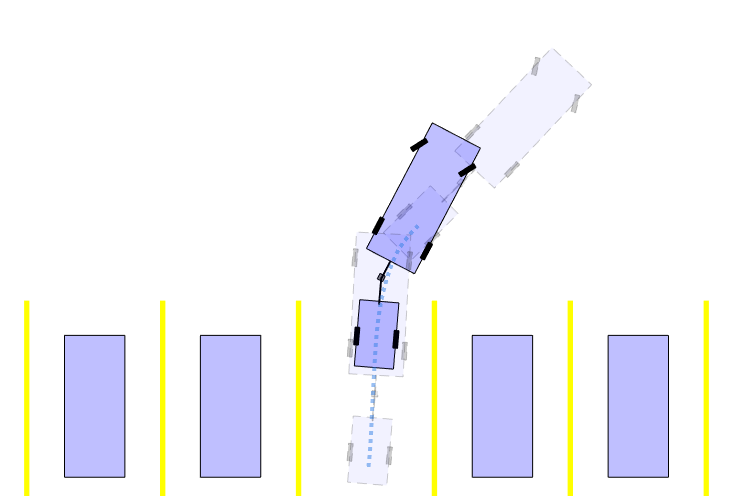
\includegraphics[width=\textwidth]{fig/ppo/parkingIllustration.png}
         \caption{Perpendicular parking simulation}
         \label{fig:parking_trajectory_1}
     \end{subfigure}
     \hfill
     \begin{subfigure}[b]{0.4\textwidth}
         \centering
         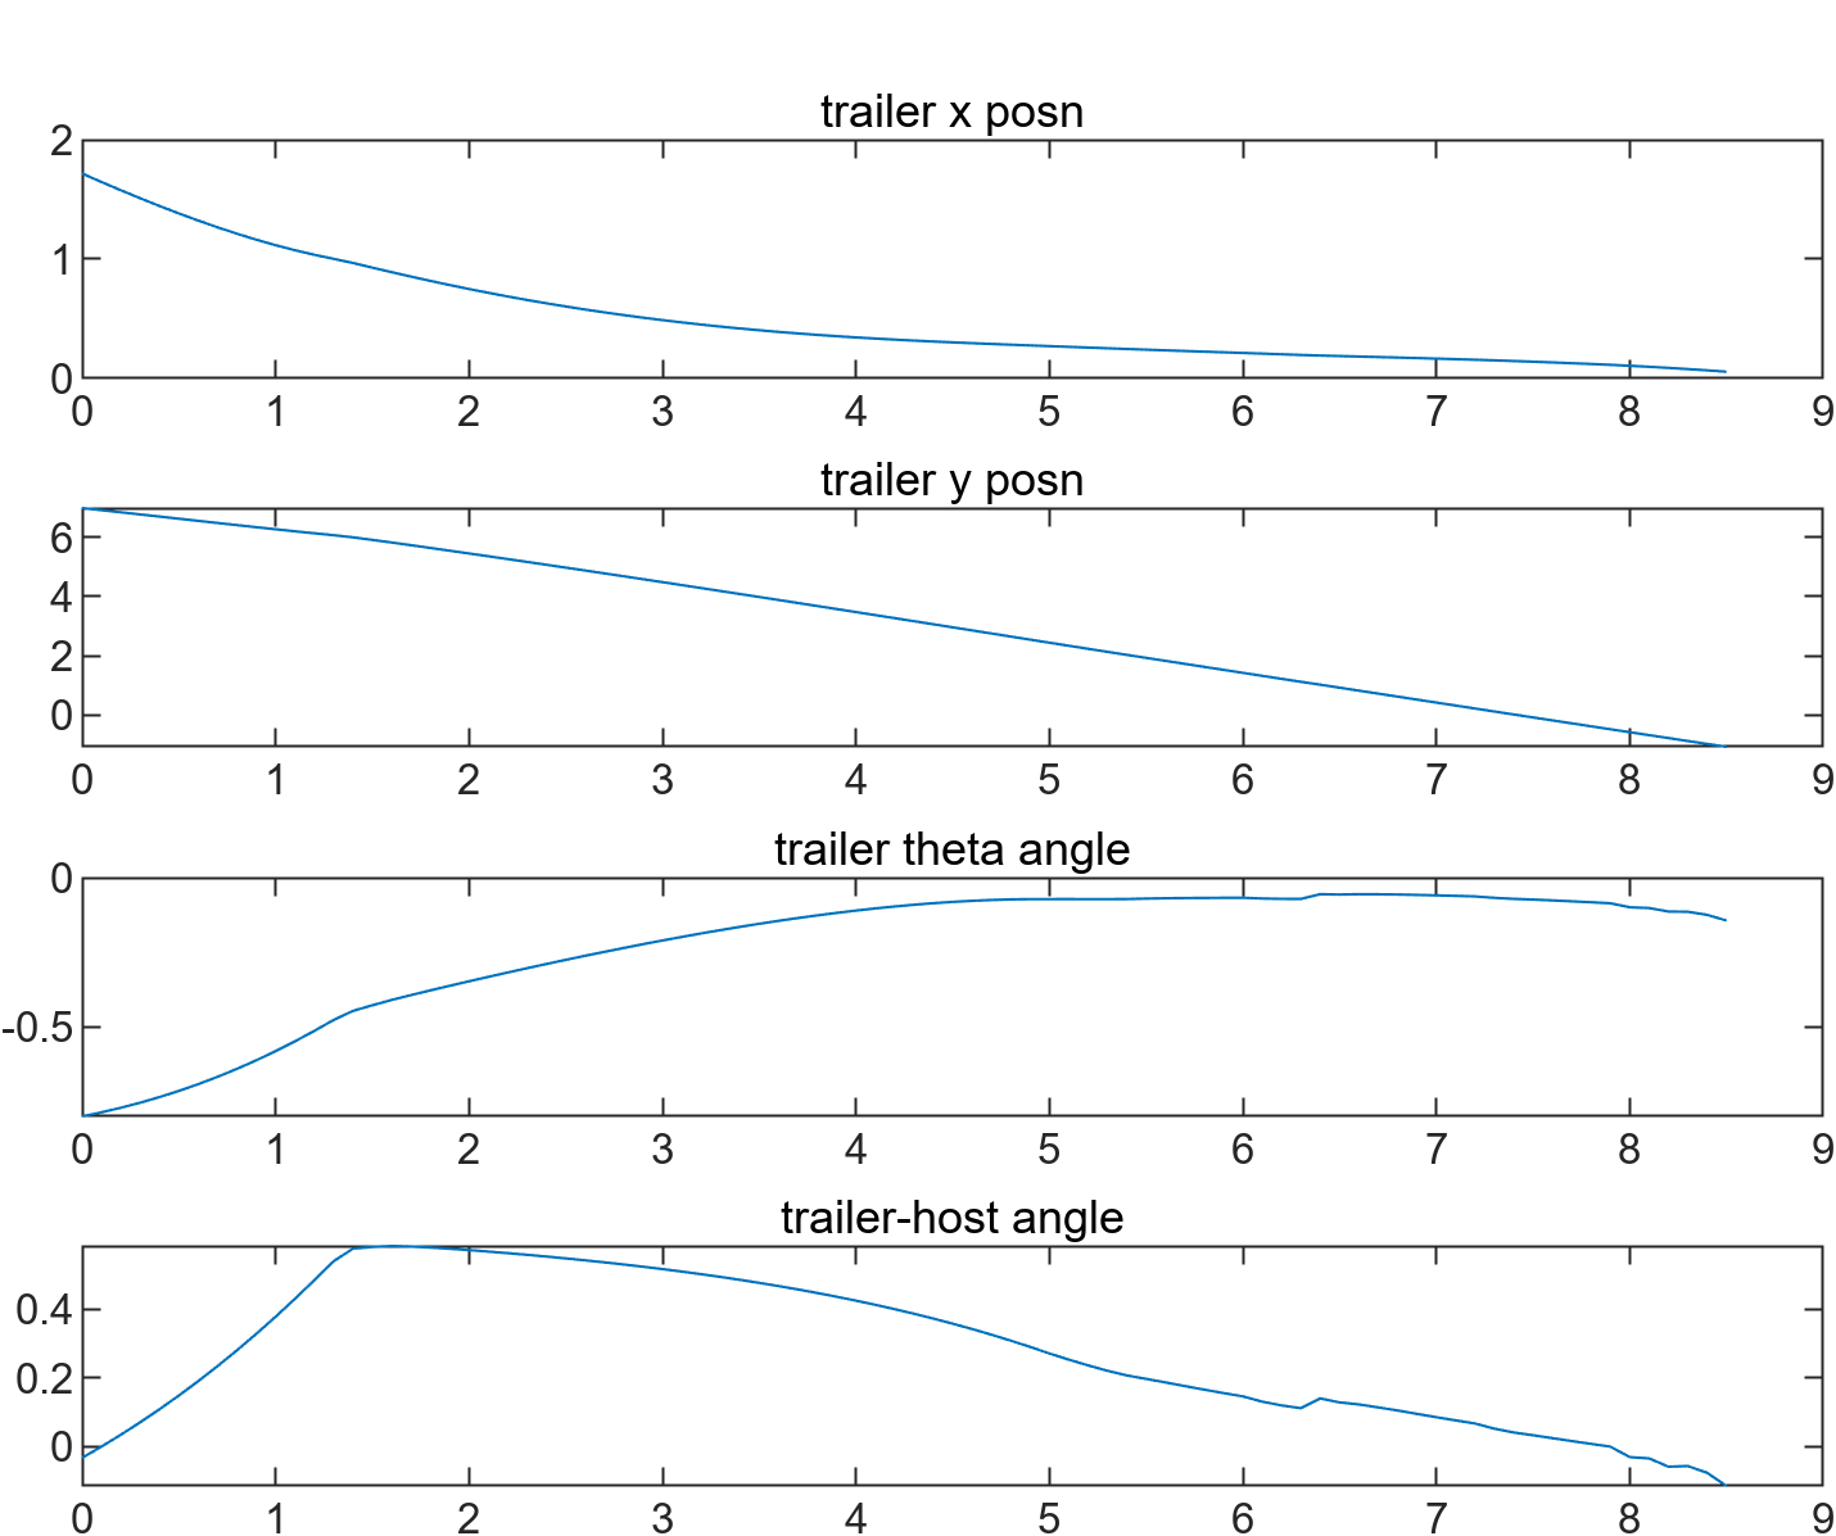
\includegraphics[width=\textwidth]{fig/ppo/parking_system_states.png}
         \caption{Perpendicular parking system states}
         \label{fig:parking_system_states}
     \end{subfigure}
        \caption{TTWR perpendicular parking}
        \label{fig:perpendicular parking}
\end{figure}

In Figure \ref{fig:oblique parking}, the TTWR trajectory during a $45^{\circ}$ oblique parking simulation is depicted. Similarly, the starting positions are initialized with a certain degree of noise, and the proposed methods successfully parked the TTWR system, ensuring jackknife prevention and obstacle evasion.

\begin{figure}
     \centering
     \begin{subfigure}[b]{0.4\textwidth}
         \centering
            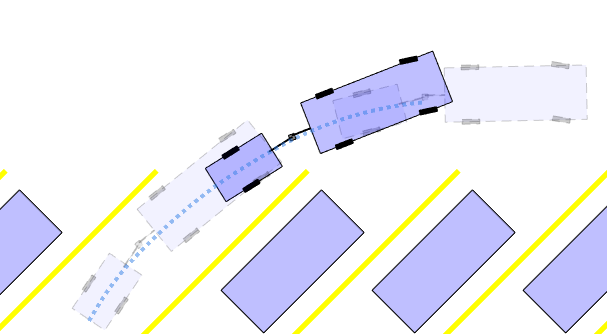
\includegraphics[width=\textwidth]{fig/ppo/parkingIllustration_oblique.png}
            \caption{Oblique parking system states}
            \label{fig:parking_trajectory_oblique_illustration}
     \end{subfigure}
     \hfill
     \begin{subfigure}[b]{0.4\textwidth}
         \centering
            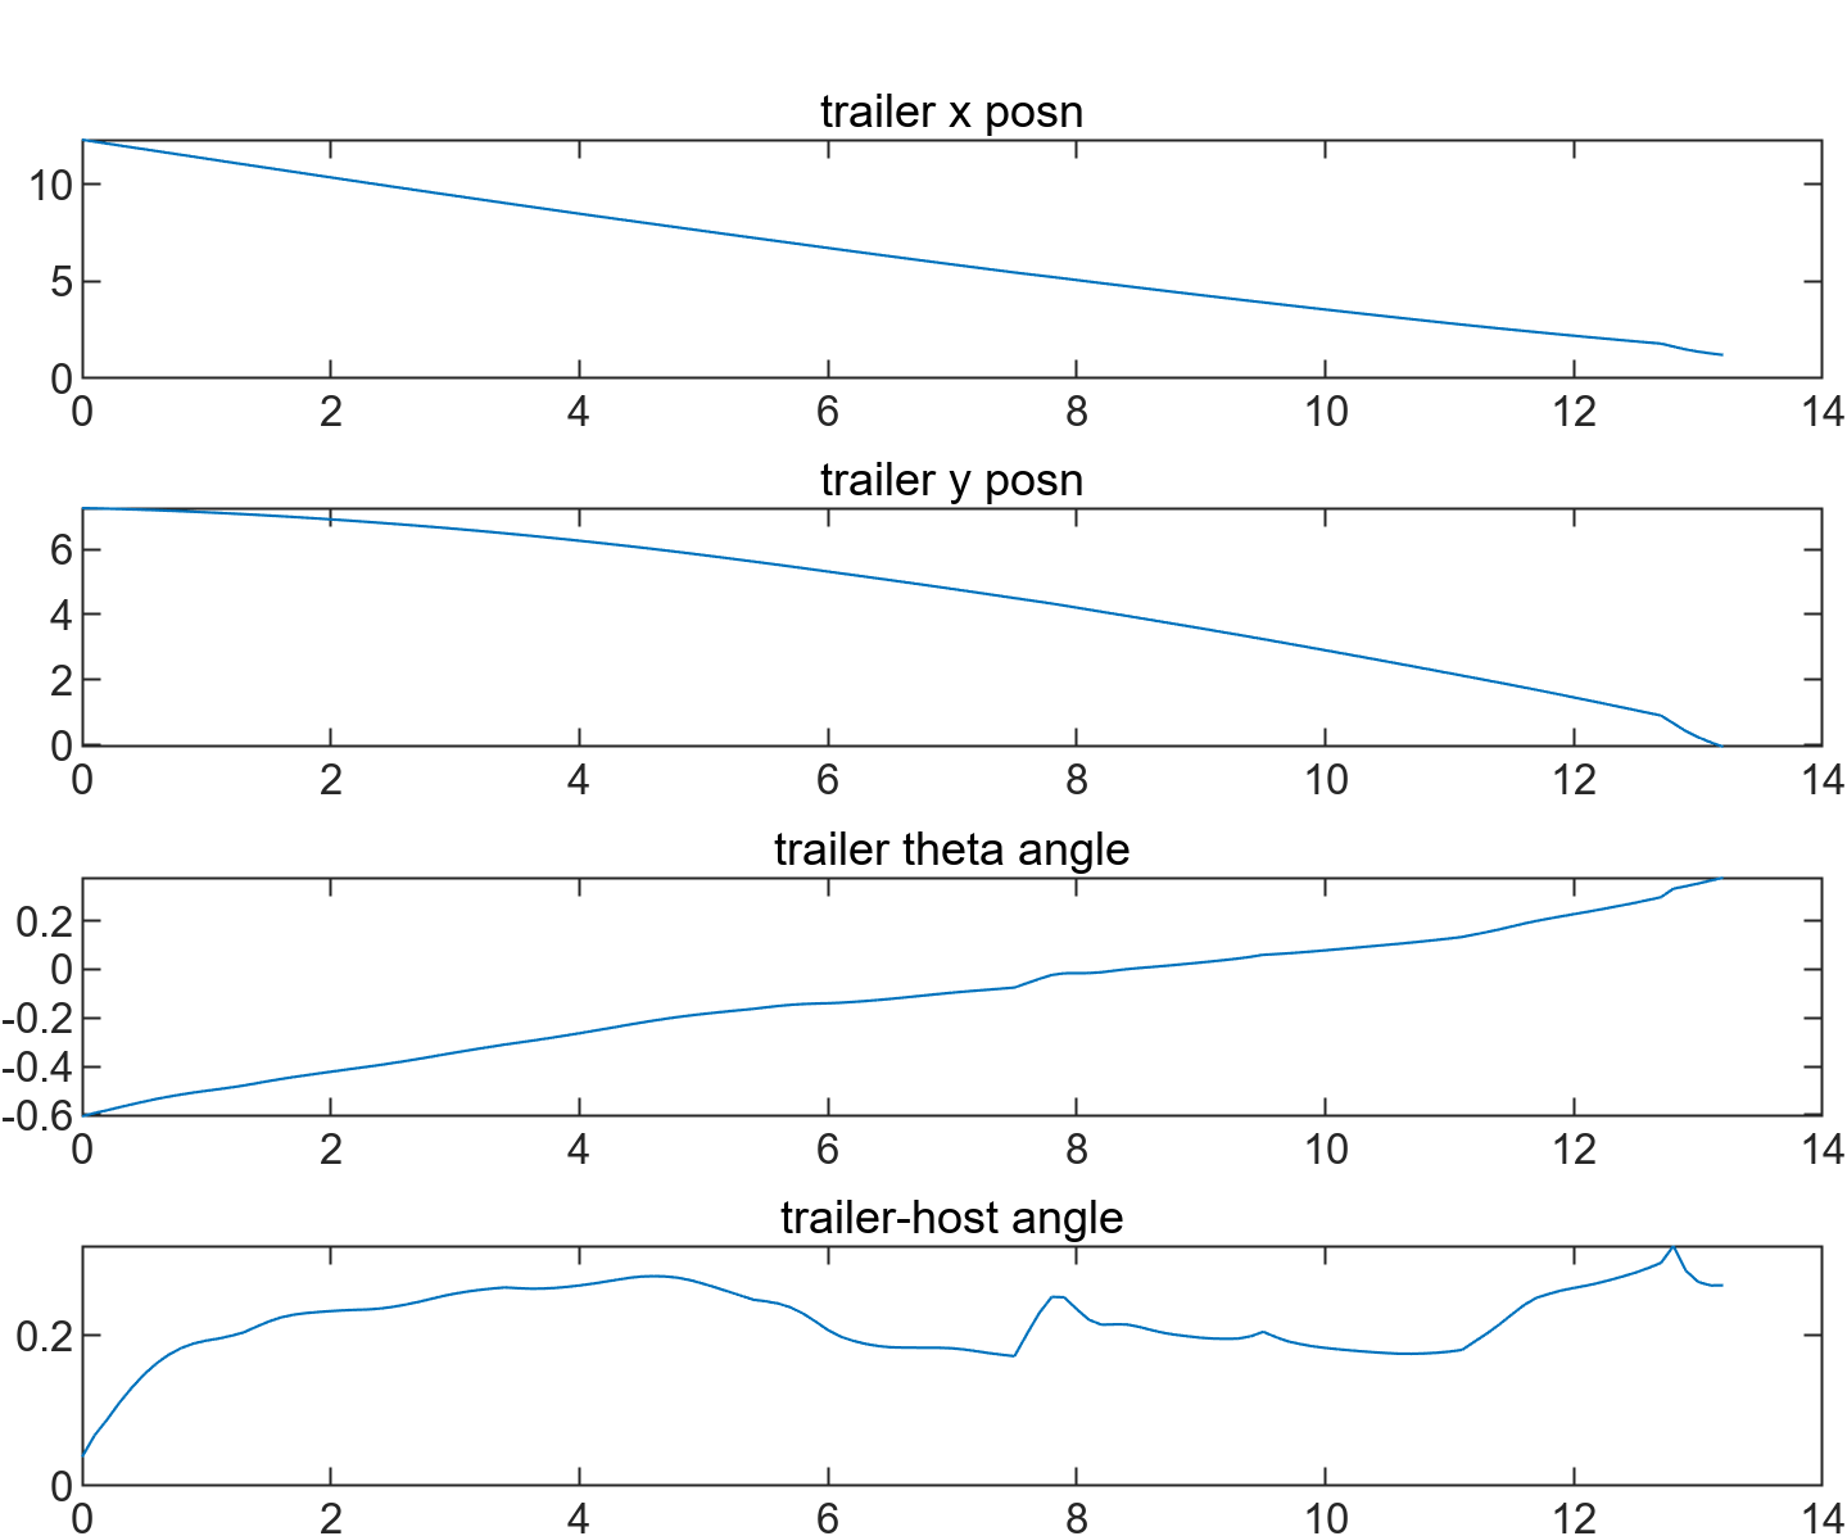
\includegraphics[width=\textwidth]{fig/ppo/parking_system_states_oblique.png}
            \caption{Oblique parking system states}
            \label{fig:parking_system_states_oblique}
     \end{subfigure}
        \caption{TTWR oblique parking}
        \label{fig:oblique parking}
\end{figure}


\section{Trajectory state model-based reinforcement learning for TTWR reverse parking}
\label{section: Trajectory state model-based reinforcement learning for TTWR reverse parking}

* this section is from the submitted second paper which does not provide citation for now.

By employing the trajectory state prediction model as the foundation model to interact with the Proximal Policy Optimization framework, we enable reversible access to the Markov Decision Process dynamics and help the PPO to better estimate vehicle dynamics used for controller. A numerical simulation is conducted to demonstrate the trajectory following accuracy of the proposed methodology compared with popular industry control methods such as linear–quadratic regulator. Our results indicate that the proposed hybrid trajectory model based approach not only reduces the need for extensive data collection but also achieves similar control accuracy, suggesting a promising direction for future research in autonomous vehicle control, emphasizing the need for efficient, adaptable, and robust learning algorithms.

\begin{figure}[h]
    \centering
    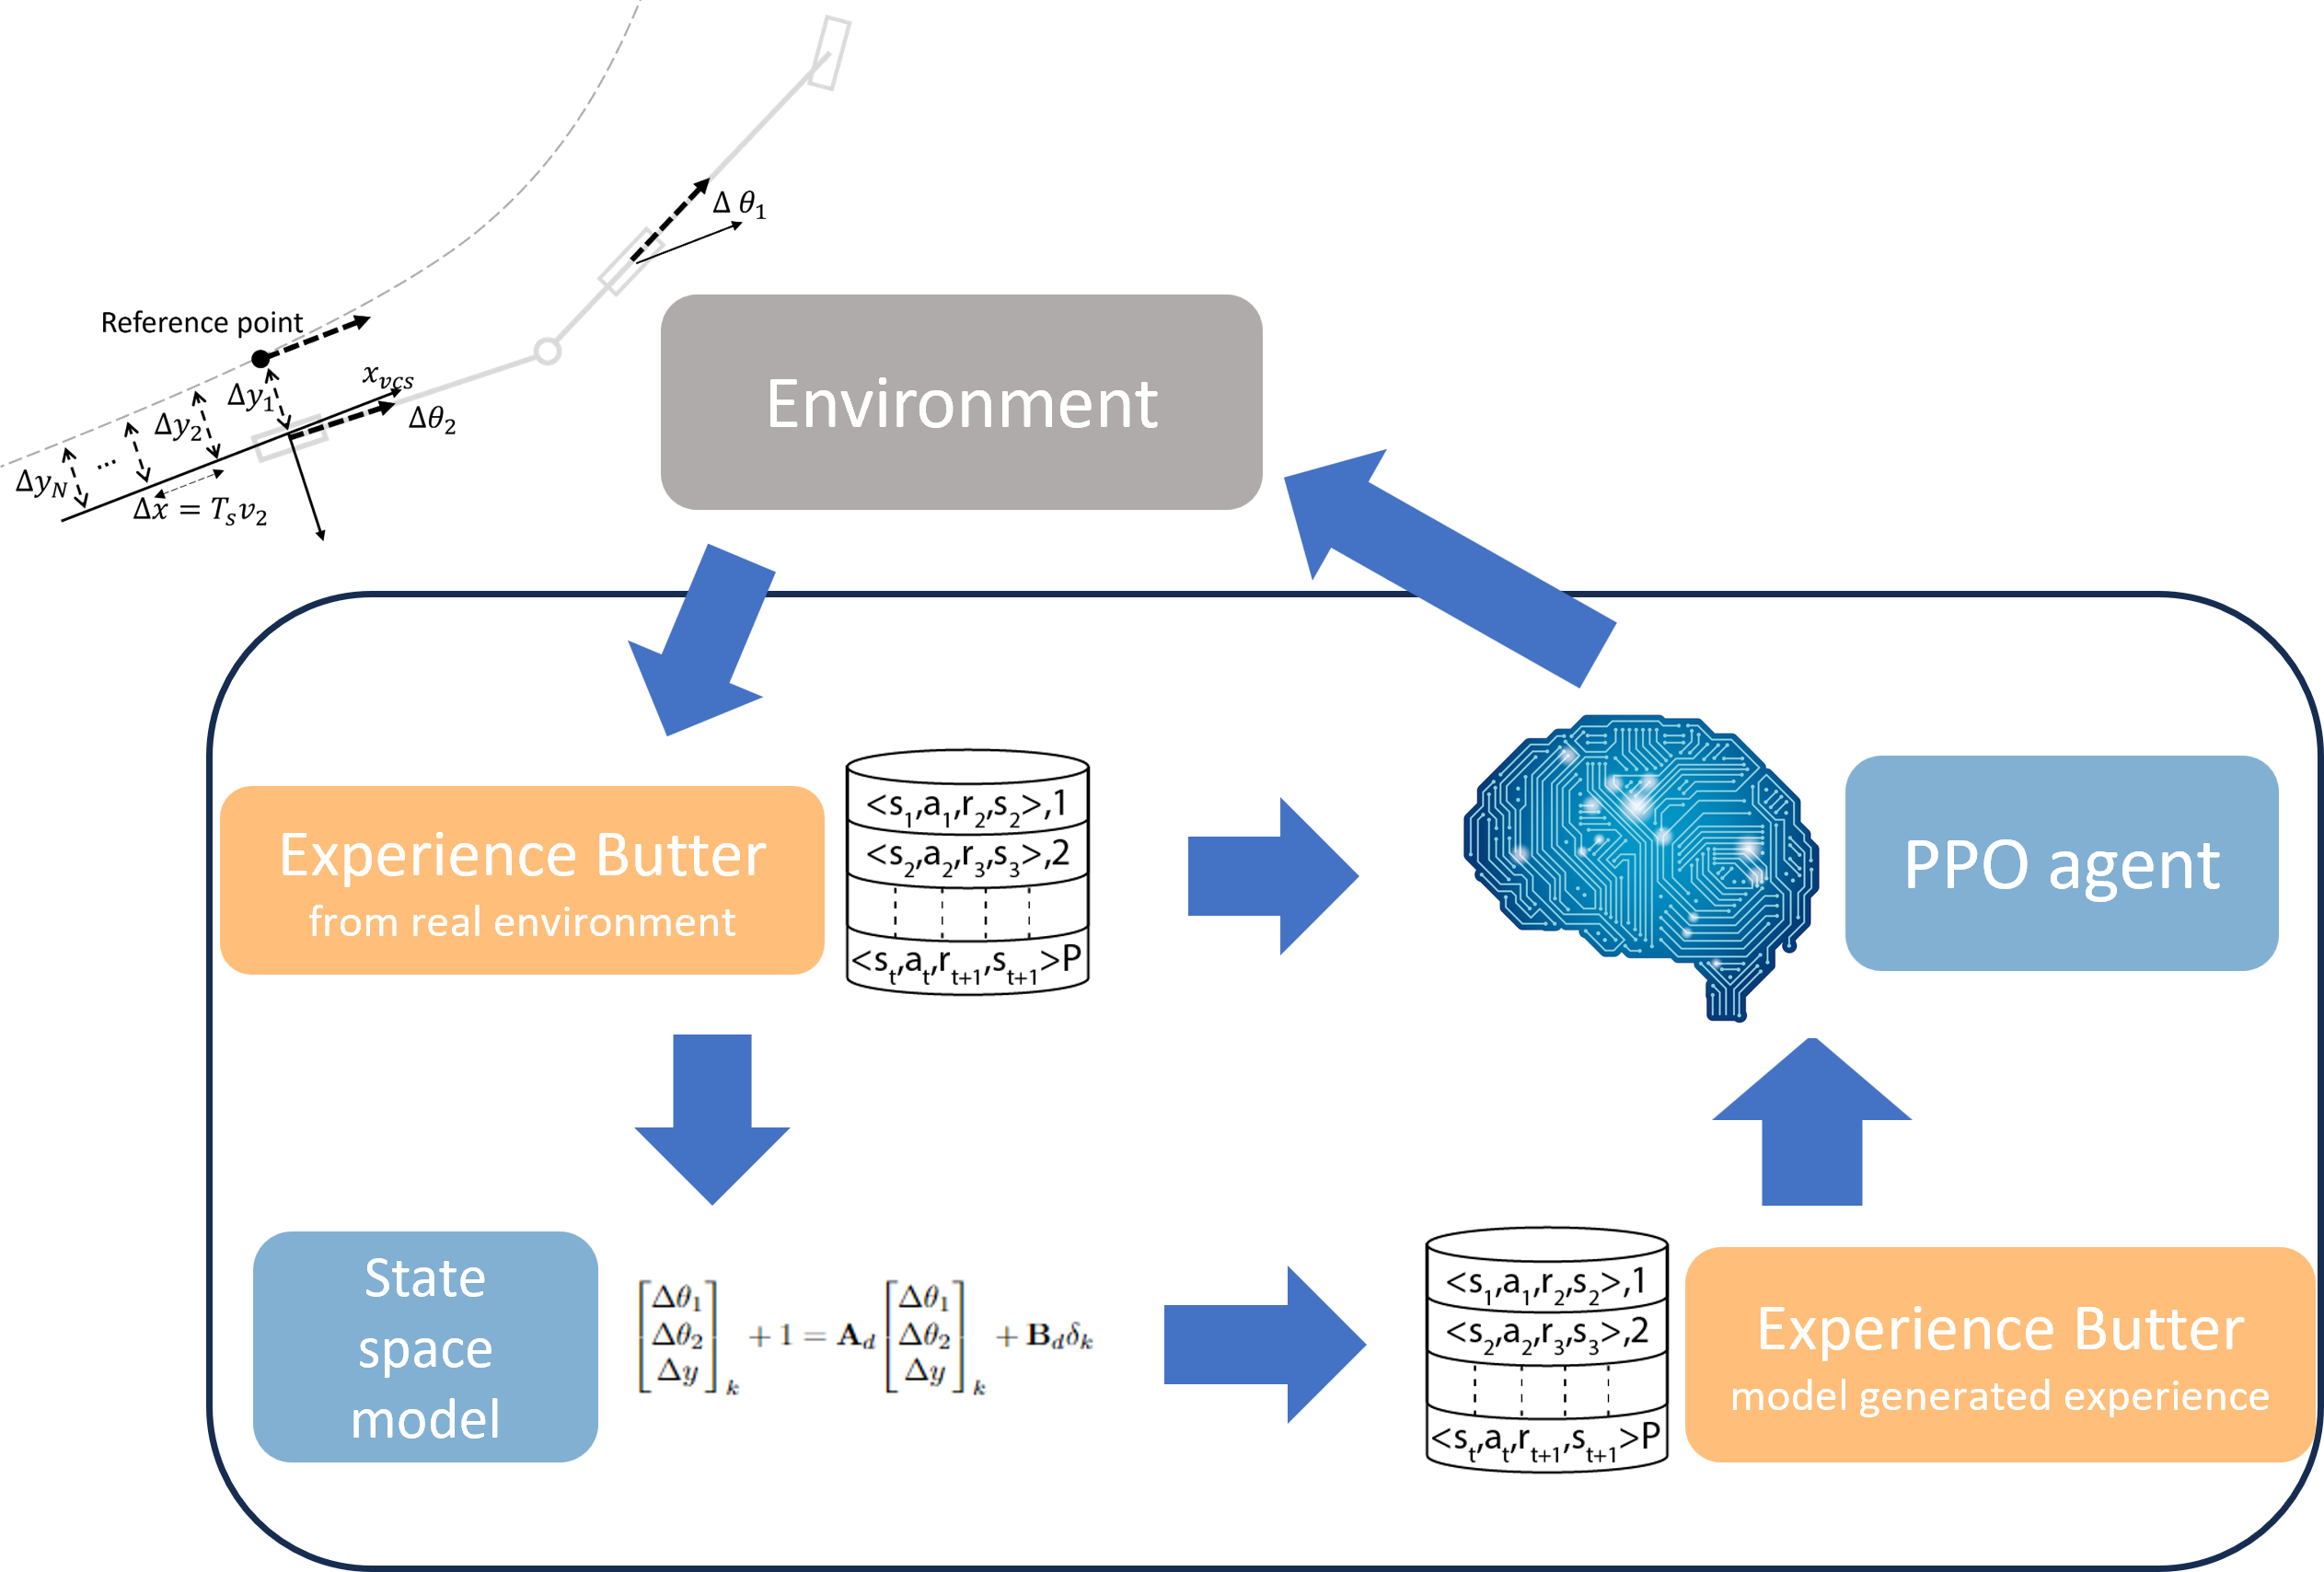
\includegraphics[width=0.8\linewidth]{fig/known mbrl schema.png}
    \caption{The MBRl structure with Dubins trajectory model generator}
    \label{fig: The MBRl structure with Dubins trajectory model generator}
\end{figure}

While model-free deep reinforcement learning has achieved remarkable successes across various domains, its application remains limited by substantial sample inefficiency and a lack of interpretability. Model-based reinforcement learning algorithms are generally regarded as being more efficient, the model-based policy search methods tackle the challenge of sample inefficiency by utilizing observed trajectories to construct a predictive model of the robot's dynamics and interactions with its surroundings \cite{schulman2015trust}. However, previous works have relied on straightforward function approximators \cite{lioutikov2014sample} or Bayesian models \cite{deisenroth2011pilco} to maintain sample efficiency and prevent overfitting. The application of these methods to diverse and intricate high-dimensional tasks is challenging. Efforts to address these issues have included the use of large-scale neural networks to capture the intricate dynamics typical of deep reinforcement learning benchmarks. However, these models often require extended training periods and struggle with transferability and interpretability \cite{nagabandi2018neural}, which confines the application scope of these models to tasks with relatively static scenarios and assignments.

By integrating the Dubin path planning with preview control, we build the system dynamics model to represent the environment interaction, where the preview distance control is also applied. In Figure \ref{fig:Vehicle kinematics model with reference}, the first $N$ preview reference points and the deviation value are plotted within the trailer VCS, and the reference error value for each preview reference sample is computed and denoted by $(\theta_{1_k}, \theta_{2_k}, y_k)$, $\Delta x$ is the sampling interval and $T_s$ is the simulation step time. Therefor, the $N$ preview sample points can be computed by:

\begin{equation} 
 {\begin{bmatrix}
    \Delta \theta_1 \\ \Delta \theta_2 \\ \Delta y
\end{bmatrix}}_k+1 = \mathbf{A}_d {\begin{bmatrix}
    \Delta \theta_1 \\ \Delta \theta_2 \\ \Delta y
\end{bmatrix}}_k + \mathbf{B}_d \delta_k
\end{equation}
where
\begin{flalign*}
A_r&=\left[\begin{array}{ccccc}
0 & 1 & 0 & \cdots & 0 \\
0 & 0 & 1 & \cdots & 0 \\
\vdots & \vdots & \vdots & \ddots & \vdots \\
0 & 0 & 0 & \cdots & 1 \\
0 & 0 & 0 & \cdots & 0
\end{array}\right]_{(N \times N)} \quad 
\end{flalign*}
and
\begin{flalign*}
B_r&=\left[\begin{array}{c}
0 \\
0 \\
0 \\
\vdots \\
1
\end{array}\right]_{(N \times 1)}
\end{flalign*}
\begin{figure}[h]
\centering
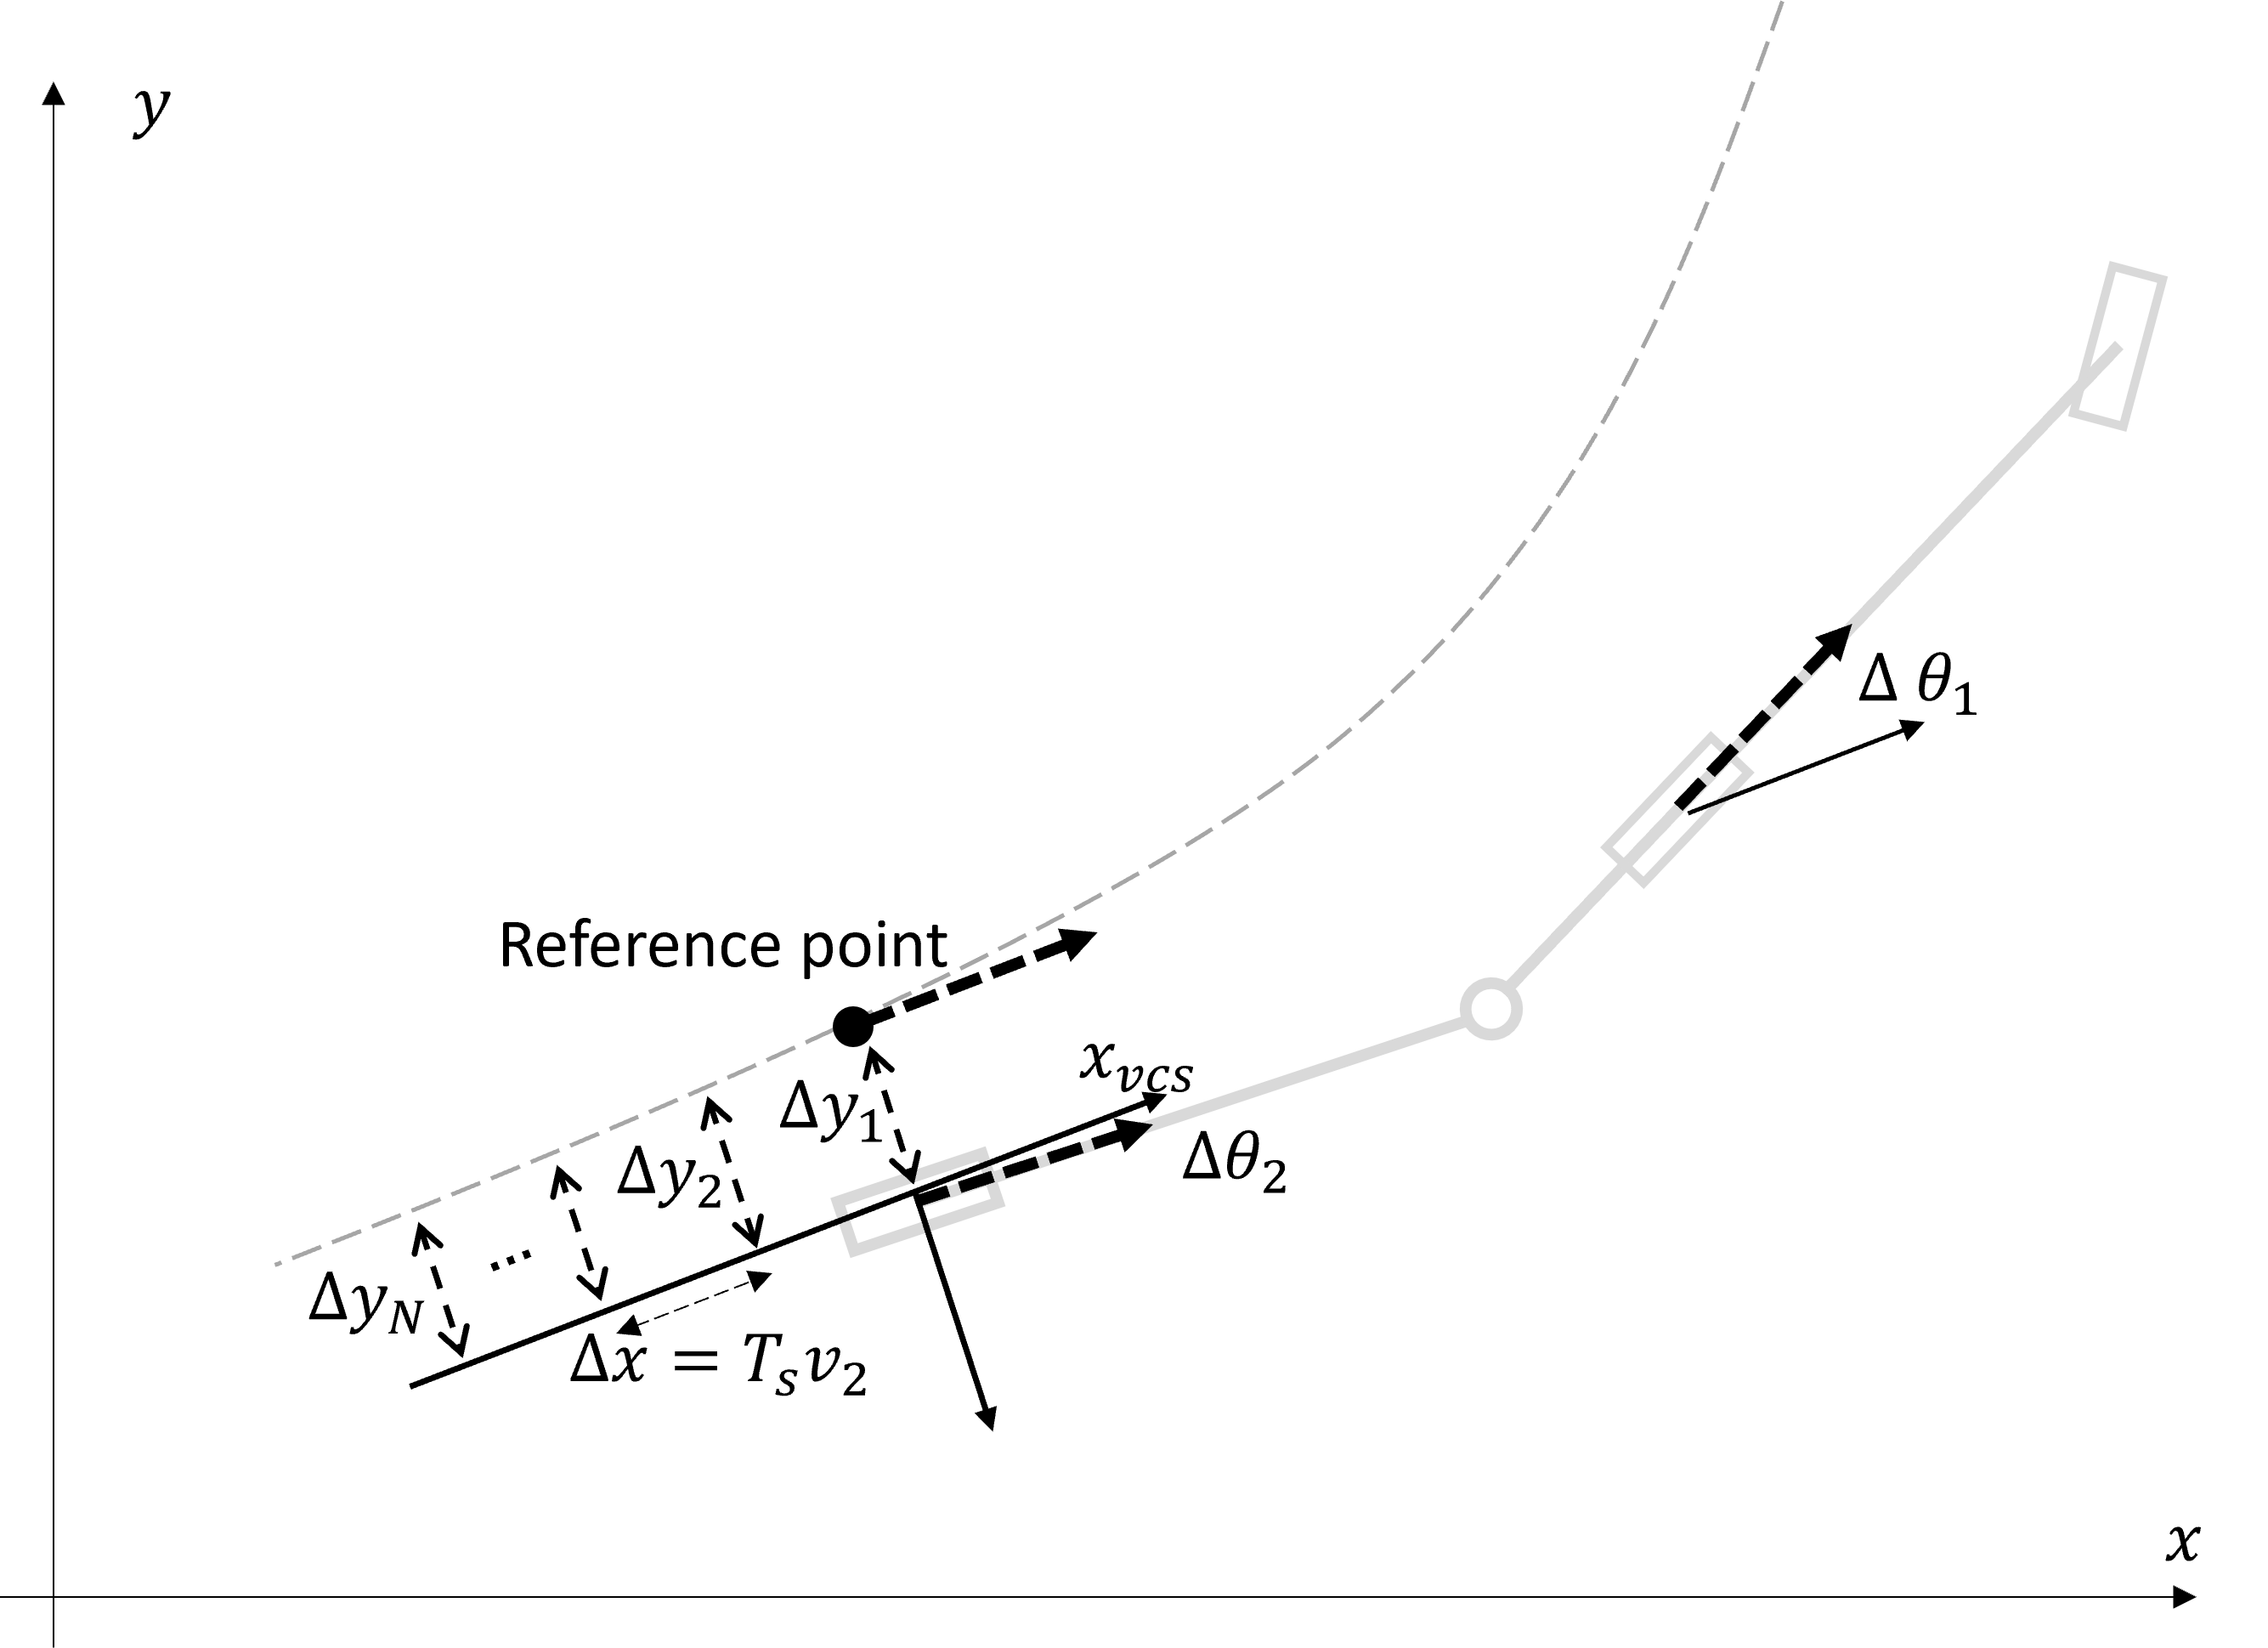
\includegraphics[width=0.8\linewidth]{fig/knownMBRL/lateral distance error.png}
\caption{Vehicle kinematics model with reference}
\label{fig:Vehicle kinematics model with reference}
\end{figure}

We evaluate the effectiveness of the proposed learning strategy using the benchmark platform across various vehicle setups for trajectory tracking tasks. The initialization of the trajectory planning and motion prediction models were based on the kinematic state space model of the vehicles which requires a single calibration for each agent. Subsequently, these models networks can be transferred and re-trained during operation to manage distinct tasks for changing vehicle configurations. The adaptability of our method was evident as it successfully handled new challenges during testing, such as managing trailers with increased overhang length which introduced more intricate dynamics.


\begin{figure}[htbp]
\centerline{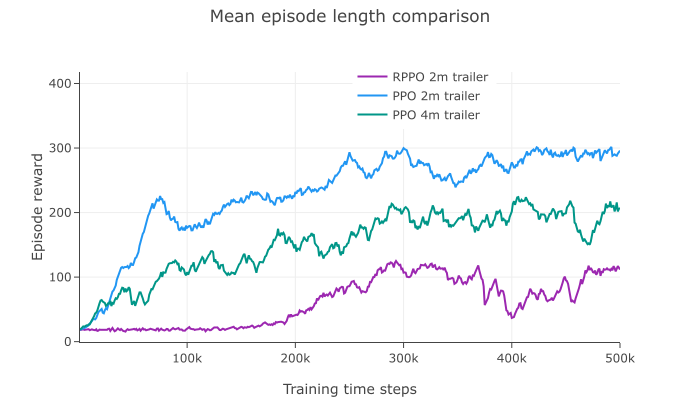
\includegraphics[width=0.8\linewidth]{fig/knownMBRL/Mean episode length.png}}
\caption{Mean episode length comparison between RPPO training on 2 meters trailer, PPO training on both 2 meters and 4 meters trailer}
\label{fig:Mean episode length}
\end{figure}

Figure \ref{fig:Mean episode length} compares the mean episode lengths for PPO-trained agents with 2-meter and 4-meter trailers as well as an RPPO-trained agent trained with 2-meter trailer. The PPO agent trained with a shorter trailer shows better performance, achieving efficient parking after 250,000 training steps. In contrast, the longer trailer brings more complexity for reverse driving maneuvering, which leads to a slower training, although it achieves similar parking success rate and rewards in \ref{fig:Mean episodic training reward}. However, the success rate of RPPO algorithm is under $50\%$ and the training takes more steps, possibly due to vanishing gradients and the intricate nature of the task's delayed rewards.

\begin{figure}[htbp]
\centerline{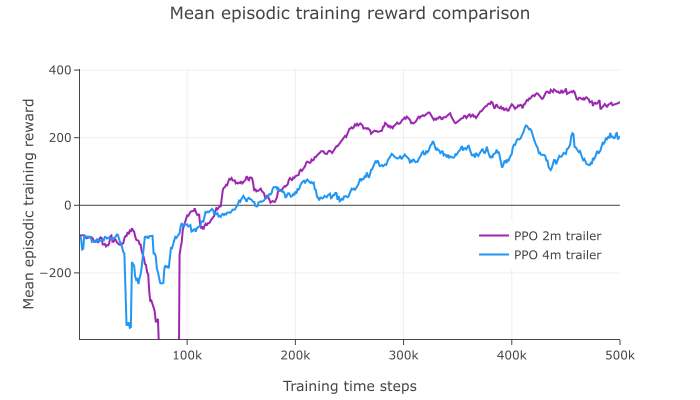
\includegraphics[width=0.8\linewidth]{fig/knownMBRL/Mean episodic training reward.png}}
\caption{Mean episode training reward comparison between PPO training on both 2 meters and 4 meters trailer}
\label{fig:Mean episodic training reward}
\end{figure}

Figure \ref{fig:Mean episodic training reward} shows that the PPO with a 2-meters trailer is able to achieving stable rewards by 250,000 steps. The training of 4m trailer's catches up by 300k steps, reflecting the added complexity in controlling longer trailers and the consequent need for extended training to refine the parking maneuvers.

\begin{figure}[htbp]
\centerline{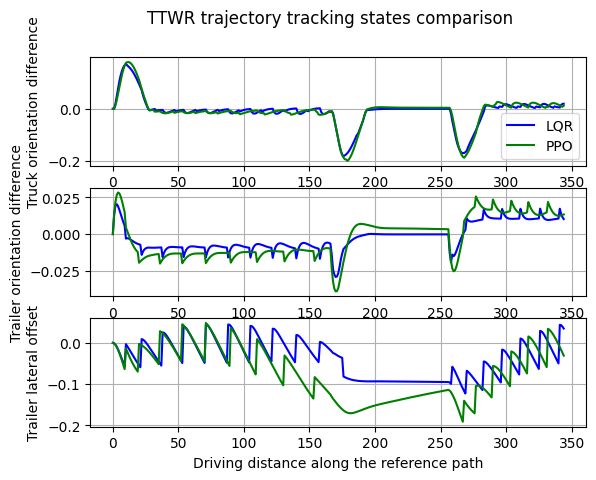
\includegraphics[width=0.8\linewidth]{fig/knownMBRL/comparison of lqr ppo.png}}
\caption{The comparison of LQR controller and proposed algorithm controlling normal 2m trailer v.s. reference trajectory orientation error, trailer orientation error, and trailer lateral offset error}
\label{fig: parking error comparison}
\end{figure}

\begin{figure}[htbp]
    \centerline{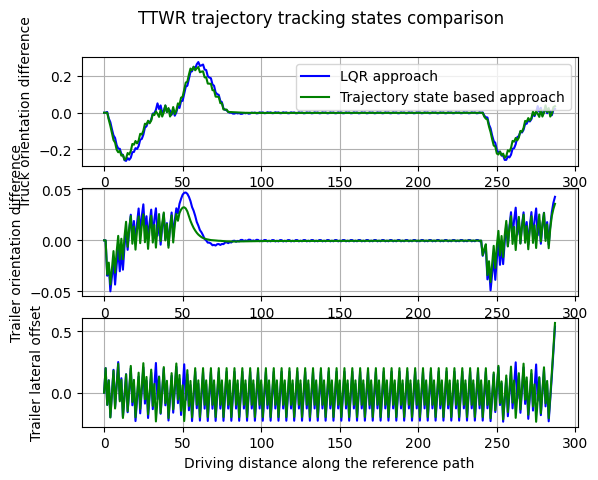
\includegraphics[width=0.8\linewidth]{fig/knownMBRL/comparison of lqr ppo extended vehicle.png}}
    \caption{The comparison of LQR controller and proposed algorithm controlling extended trailer v.s. reference trajectory orientation error, trailer orientation error, and trailer lateral offset error}
    \label{fig: parking error comparison of extended trailer}
\end{figure}

Figure \ref{fig: parking error comparison} compares the LQR controller with the proposed algorithm regarding truck orientation error, trailer orientation error, and lateral offset error. For a 2-meter trailer which is popular in North America market which handles most moving tasks, the performance of both systems is closely matched, with the lateral offset consistently maintained below 0.2 meters. The result shows the proposed algorithm's high tracking accuracy and suggests its potential effectiveness in practical scenarios.

Figure \ref{fig: parking error comparison of extended trailer} presents a comparative analysis of the LQR controller and the proposed algorithm, applied to a 5-meter extended trailer designed for heavy-duty tasks. Both controllers successfully follow the given trajectory; however, the proposed algorithm demonstrates slightly better performance in orientation tracking with smaller errors. This indicates enhanced adaptability of the proposed algorithm in contrast to the LQR controller, which relies on fixed feedback gains.

% Chapter 6
\chapter{\leavevmode\newline Dissertation Work Plan }
\chaptermark{Heading on Chapter Pages}
\label{chap: Dissertation Work Plan}

\section{Dissertation Progresses Work}


\section*{Phase 1: Preliminary Analysis and Model Development }

\begin{enumerate}
    \item \textbf{Literature Review}:
    \begin{itemize}
        \item Study existing literature on truck-trailer dynamics, reverse parking algorithms, and model-based reinforcement learning applications in vehicle control.
        \item Identify gaps in current methodologies and potential improvements.
    \end{itemize}
    
    \item \textbf{Data Collection}:
    \begin{itemize}
        \item Gather data on truck-trailer dynamics during reverse parking maneuvers. This can include sensor data, camera feeds, and other relevant telemetry.
        \item Use simulators if real-world data collection is challenging or risky.
    \end{itemize}
    
    \item \textbf{Model Development}:
    \begin{itemize}
        \item Develop a dynamic model of the truck-trailer system. This model should capture the kinematics and dynamics of reverse parking.
        \item Validate the model using collected data or through simulation environments.
    \end{itemize}
\end{enumerate}

\section*{Phase 2: Reinforcement Learning Framework and Simulation }
\begin{enumerate}
    \item \textbf{RL Environment Setup}:
    \begin{itemize}
        \item Define the state space (positions, angles, velocities), action space (steering angles, acceleration), and reward function (based on parking accuracy, safety, and maneuver time).
        \item Set up terminal conditions, such as successful parking or collision scenarios.
    \end{itemize}
    
    \item \textbf{Algorithm Selection and Development}:
    \begin{itemize}
        \item Choose an appropriate model-based RL algorithm. Consider algorithms that can efficiently utilize the truck-trailer model to simulate future trajectories.
        \item Implement the algorithm and integrate it with the dynamic model.
    \end{itemize}
    
    \item \textbf{Simulation and Testing}:
    \begin{itemize}
        \item Use a high-fidelity simulator to test the RL agent's performance. Ensure the simulator can accurately replicate real-world parking scenarios.
        \item Iteratively train the agent, refining the model and RL algorithm based on simulation results.
    \end{itemize}
\end{enumerate}

\section*{Phase 3: Comparative Analysis with Other Control Algorithms}
\begin{enumerate}
    \item \textbf{Selection of Control Algorithms}:
    \begin{itemize}
        \item Identify other prominent control algorithms used for truck-trailer reverse parking, such as LQR, MPC, or other traditional methods.
    \end{itemize}
    
    \item \textbf{Implementation and Testing}:
    \begin{itemize}
        \item Implement the selected control algorithms in the simulation environment.
        \item Test each algorithm under similar conditions to ensure a fair comparison.
    \end{itemize}
    
    \item \textbf{Performance Evaluation}:
    \begin{itemize}
        \item Evaluate the performance of each algorithm based on criteria like parking accuracy, safety, time taken, and control smoothness.
        \item Compare the results of the model-based RL approach with the results of the other algorithms.
    \end{itemize}
    
    \item \textbf{Analysis and Reporting}:
    \begin{itemize}
        \item Analyze the strengths and weaknesses of the model-based RL approach in comparison to the other algorithms.
        \item Document findings, insights, and potential areas for improvement or further research.
    \end{itemize}
\end{enumerate}


\section{Deliverables}
This research aims to explore the potential of model-based reinforcement learning (MBRL) in the domain of truck-trailer reverse parking control. The objective is to develop an efficient and robust control strategy that can outperform traditional methods. The deliverables outlined below provide a comprehensive overview of the expected outcomes, tools, and documentation that will be produced during the research process.

\begin{enumerate}
    \item \textbf{Dynamic Model of the Truck-Trailer System}:
    \begin{itemize}
        \item A mathematical representation capturing the kinematics and dynamics of the truck-trailer during reverse parking maneuvers.
        \item Validation results comparing the model's predictions with simulation or real-world data.
    \end{itemize}
    
    \item \textbf{Benchmark Control Algorithms based on Trarditional Algorithms}:
    \begin{itemize}
        \item Dubins path planning for reverse parking path generation
        \item A* path planning for spot search and trajectory generation
        \item LQR controller
        \item MPC controller
    \end{itemize}
    
    \item \textbf{Reinforcement Learning Framework}:
    \begin{itemize}
        \item Detailed documentation of the chosen DQN RL algorithm, including its advantages and limitations.
        \item Detailed documentation of the chosen PPO RL algorithm, including its advantages and limitations.
        \item Detailed documentation of the chosen model-based RL algorithm, including its advantages and limitations.
        \item Source code of the implemented RL algorithm, accompanied by comments and usage instructions.
    \end{itemize}
    
    \item \textbf{Simulation Results}:
    \begin{itemize}
        \item A comprehensive report detailing the performance of the RL agent in various simulated scenarios.
        \item Visual aids such as graphs, plots, and possibly videos showcasing the agent's performance.
    \end{itemize}
    
    \item \textbf{Comparative Analysis}:
    \begin{itemize}
        \item A structured comparison between the MBRL approach and other control algorithms.
        \item Performance metrics, challenges faced, and potential areas of improvement for each method.
    \end{itemize}
    
    \item \textbf{Software Tools and Utilities}:
    \begin{itemize}
        \item Any custom software or utilities developed during the research, including simulation tools, data processing scripts, and visualization aids.
        \item Documentation and user manuals for these tools, ensuring future researchers or collaborators can utilize them effectively.
    \end{itemize}
    
    \item \textbf{Final Thesis}:
    \begin{itemize}
        \item A comprehensive document detailing the entire research process, methodologies, results, and conclusions.
        \item Recommendations for future research or potential real-world applications of the developed MBRL approach.
    \end{itemize}
\end{enumerate}

\section{Research Schedule}

The following is the coursework layout and dissertation schedule separated by milestones and months:

\begin{enumerate}
\item \textbf{Model Development and Validation (September 2023 - December 2023)}
\begin{itemize}
    \item Develop and validate the dynamic model of the truck-trailer system.
    \item Begin preliminary work on the benchmark control algorithms based on traditional methods.
\end{itemize}

\item \textbf{Reinforcement Learning Framework Development (November 2023 - March 2024)}
\begin{itemize}
    \item Implement and test the chosen DQN, TD3, and model-based RL algorithms.
    \item Start simulations and gather initial results.
\end{itemize}

\item \textbf{Comparative Analysis and Refinement (April 2024 - May 2024)}
\begin{itemize}
    \item Conduct a structured comparison between the MBRL approach and other control algorithms.
    \item Refine and optimize the RL algorithms based on the comparative analysis.
\end{itemize}

\item \textbf{Finalization and Thesis Writing (July 2024 - August 2024)}
\begin{itemize}
    \item Finalize all research components, including software tools and utilities.
    \item Write, review, and finalize the PhD thesis.
\end{itemize}
\end{enumerate}



\clearpage


% Reference
%========================================
\addcontentsline{toc}{chapter}{References}
\begin{singlespace}
	\setlength\bibitemsep{\baselineskip}
	\printbibliography[title={References}]
\end{singlespace}
\clearpage

% Appendices
% \begin{appendices}

\addtocontents{toc}{\protect\renewcommand{\protect\cftchappresnum}{\appendixname\space}}
\addtocontents{toc}{\protect\renewcommand{\protect\cftchapnumwidth}{7em}}

\chapter{This is Appendix A}
\lipsum[1]

\end{appendices}
% \clearpage

% \begin{appendices}

\addtocontents{toc}{\protect\renewcommand{\protect\cftchappresnum}{\appendixname\space}}
\addtocontents{toc}{\protect\renewcommand{\protect\cftchapnumwidth}{7em}}

\chapter{This is Appendix B}
\lipsum[1]

\end{appendices}
% \clearpage

\end{document}